% diode_stack_design_guidelines.tex
% Design guidelines: series-connected diode stacks for medium-voltage six-pulse rectifiers
% pwr-control template (AAA_template_latex_settings); numbers and figures of the worked example:
% diode_stack_calc.py (with diode_stack_sim.py and diode_stack_recovery.py), which writes diode_stack_values.tex
% Compile: pdflatex diode_stack_design_guidelines.tex  (twice, for references)
% Rev. 00 - November 2026 - first issue
\documentclass[10pt,a4paper]{scrartcl}
% ===================== PACKAGES =====================
\usepackage[british]{babel}
\usepackage[tmargin=1in, bmargin=1in, lmargin=0.75in, rmargin=0.75in]{geometry}
\usepackage[dvipsnames,table]{xcolor}  % prima di tikz, listings, ecc.

\usepackage{tikz}
\usepackage{graphicx}
\usepackage{pgfplots}
\pgfplotsset{width=12cm, compat=1.9}
\usepackage{setspace}
\usepackage{chemmacros}
\usepackage{chemfig}
\usepackage{esint}
\usepackage{tabularray}
\usepackage{makeidx}
\usepackage{epstopdf}
\usepackage{amssymb}
\usepackage{mathrsfs}
\usepackage{bm}
\usepackage{amsmath}
\usepackage{enumitem}
\usepackage[english]{varioref}
\usepackage{lipsum}
\usepackage{fancyhdr}
\usepackage{float}
\usepackage{empheq}
\usepackage[framemethod=tikz]{mdframed}
\numberwithin{equation}{section}
\usepackage{eso-pic}
\usepackage{calc}
\usepackage{nccmath}
\usepackage{caption}
\usepackage{subcaption}
\usepackage{gensymb}
\usepackage{amsfonts, amsthm, epsfig, epstopdf, titling, url, array}
\usepackage{tabularx}
\usepackage{makecell}
\usepackage{booktabs}
\usepackage{array}
\usepackage{siunitx}
\sisetup{input-digits=0123456789\pi}
\usepackage[symbol]{footmisc}
\usepackage{multicol}
\usepackage{boondox-cal}
\usepackage{blindtext}
\usepackage{changepage}
\usepackage{nomencl}
\usepackage{hyperref}
\usepackage{xurl}
\usepackage{ragged2e}
\usepackage[version=4]{mhchem}  % ← conflitto di opzioni
\usepackage{longtable}
\usepackage{chemformula}
\usetikzlibrary{arrows.meta,positioning,calc}

% ===================== SI UNITS =====================
\DeclareSIUnit\atm{atm}
\DeclareSIUnit{\var}{var}
\DeclareSIUnit{\pu}{p.u.}


% ===================== MATH OPERATORS =====================
\DeclareMathOperator{\rank}{rank}
\DeclareMathOperator{\atantwo}{atan2}
\DeclareMathOperator{\spn}{span}

% ===================== COMMANDS =====================
\newcommand{\abs}[1]{\left|#1\right|}
\newcommand{\sign}{\text{sign}}
\newcommand{\centered}[1]{\begin{tabular}{@{}l@{}} #1 \end{tabular}}

% ===================== COLORS =====================
\definecolor{mycolor1}{rgb}{0.97, 0.97, 0.97}
\definecolor{mycolor2}{rgb}{0.97, 0.97, 0.97}
\definecolor{tableShade}{gray}{0.9}

% ===================== THEOREM ENVIRONMENTS =====================
\theoremstyle{it}
\newtheorem{defn}{Definition}[section]
\newtheorem{assumption}{Assumption}[section]
\newtheorem{thm}{Theorem}[section]
\newtheorem{lemma}{Lemma}[section]
\newtheorem{corollary}{Corollary}[section]
\theoremstyle{definition}
\newtheorem{example}{Example}[section]

% ===================== CUSTOM ENVIRONMENTS =====================
\newenvironment{myitemize_1}{
	\begin{itemize}[topsep=0pt]
		\setlength{\topsep}{2pt}
		\setlength{\itemsep}{2pt}
		\setlength{\parskip}{2pt}
		\setlength{\parsep}{2pt}
	}{\end{itemize}}

\newmdenv[
innerlinewidth=0.5pt,
roundcorner=4pt,
backgroundcolor=mycolor2,
linecolor=mycolor1,
innerleftmargin=6pt,
innerrightmargin=6pt,
innertopmargin=6pt,
innerbottommargin=6pt
]{mybox}

% ===================== TABLE COLUMN TYPES =====================
\newcolumntype{Y}{>{\hsize=2\hsize}X}
\newcolumntype{Z}{>{\centering\arraybackslash\hsize=0.857\hsize}X}

% ===================== SECTION DEPTH =====================
\setcounter{secnumdepth}{3}
\setcounter{tocdepth}{3}

% ===================== PAGE STYLE =====================
\setlength{\headheight}{20pt}
\setlength{\headsep}{20pt}

\pagestyle{fancy}
\fancypagestyle{firstpage}{\rhead{}}
\fancyhead[L]{\slshape\nouppercase{\leftmark}}
\chead{}
\rhead{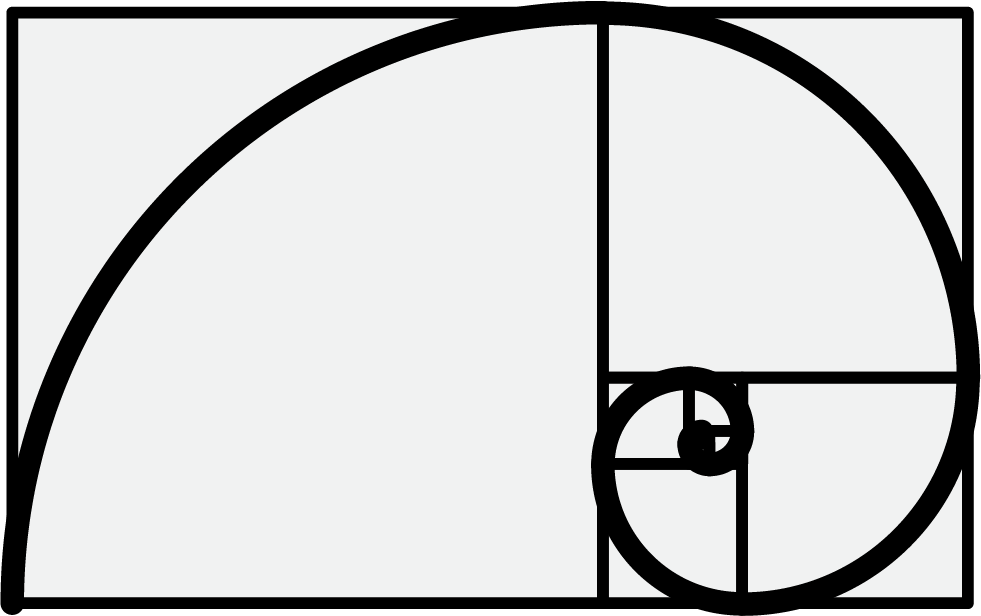
\includegraphics[height=0.75cm]{../../AAA_template_latex_settings/pwr-control_logo_doc.png}}
\lfoot{\href{http://www.pwr-control.com}{pwr-control.com}}
\cfoot{-\ \thepage\ -}
\rfoot{\textit{}}
\renewcommand{\headrulewidth}{0.4pt}
\renewcommand{\footrulewidth}{0.4pt}


\geometry{
	a4paper,
	top    = 2.5cm,
	bottom = 3.0cm,
	left   = 2.5cm,
	right  = 2.5cm
}

\hypersetup{
	colorlinks = true,
	urlcolor   = blue,
	linkcolor  = black,
	citecolor  = black
}

\pagenumbering{gobble}
\rfoot{\small Rev.~00}
\geometry{left=2.0cm, right=2.0cm}
\usepackage[european resistors, american inductors]{circuitikz}

\sisetup{per-mode=symbol,range-phrase={\text{--}},range-units=single}
\setlist{nosep}
\setlength{\parindent}{0pt}
\setlength{\parskip}{3pt}
\allowdisplaybreaks
\captionsetup{font=small,labelfont=bf}

% --- numbers of the worked example (generated by diode_stack_calc.py) ---
% generated by diode_stack_calc.py: do not edit by hand
\newcommand{\dsIdNom}{100.0}
\newcommand{\dsMuNom}{20.3}
\newcommand{\dsVdcNom}{13.09}
\newcommand{\dsVzeroNom}{4.90}
\newcommand{\dsAlphaNom}{0.176}
\newcommand{\dsTrampNom}{569}
\newcommand{\dsVhatNom}{14.14}
\newcommand{\dsVsRmsNom}{8.83}
\newcommand{\dsVsMeanNom}{6.54}
\newcommand{\dsTovNom}{1.13}
\newcommand{\dsIdMax}{110.0}
\newcommand{\dsMuMax}{20.3}
\newcommand{\dsVdcMax}{14.40}
\newcommand{\dsVzeroMax}{5.39}
\newcommand{\dsAlphaMax}{0.193}
\newcommand{\dsTrampMax}{569}
\newcommand{\dsVhatMax}{15.56}
\newcommand{\dsVsRmsMax}{9.71}
\newcommand{\dsVsMeanMax}{7.20}
\newcommand{\dsTovMax}{1.13}
\newcommand{\dsIdUkmin}{111.0}
\newcommand{\dsMuUkmin}{17.2}
\newcommand{\dsVdcUkmin}{14.52}
\newcommand{\dsVzeroUkmin}{4.59}
\newcommand{\dsAlphaUkmin}{0.231}
\newcommand{\dsTrampUkmin}{481}
\newcommand{\dsVhatUkmin}{15.56}
\newcommand{\dsVsRmsUkmin}{9.76}
\newcommand{\dsVsMeanUkmin}{7.26}
\newcommand{\dsTovUkmin}{0.95}
\newcommand{\dsIdHalf}{50.8}
\newcommand{\dsMuHalf}{14.4}
\newcommand{\dsVdcHalf}{13.29}
\newcommand{\dsVzeroHalf}{3.52}
\newcommand{\dsAlphaHalf}{0.126}
\newcommand{\dsTrampHalf}{402}
\newcommand{\dsVhatHalf}{14.14}
\newcommand{\dsVsRmsHalf}{8.91}
\newcommand{\dsVsMeanHalf}{6.65}
\newcommand{\dsTovHalf}{0.80}
\newcommand{\dsKrmsZero}{0.634}
\newcommand{\dsKrmsUZero}{0.897}
\newcommand{\dsKrmsNom}{0.624}
\newcommand{\dsLc}{13.93}
\newcommand{\dsLcMin}{9.95}
\newcommand{\dsItn}{92.4}
\newcommand{\dsRload}{130.9}
\newcommand{\dsSt}{1.6}
\newcommand{\dsUn}{10}
\newcommand{\dsUmax}{11}
\newcommand{\dsUk}{7}
\newcommand{\dsUkMin}{5}
\newcommand{\dsIdRated}{100}
\newcommand{\dsKgrid}{10}
\newcommand{\dsAlphaRatioUkmin}{1.19}
\newcommand{\dsAlphaLo}{0.13}
\newcommand{\dsAlphaHi}{0.23}
\newcommand{\dsTrampLo}{400}
\newcommand{\dsTrampHi}{570}
\newcommand{\dsVlev}{2.59}
\newcommand{\dsIlkDes}{0.97}
\newcommand{\dsRoffLim}{2.69}
\newcommand{\dsIlkRatio}{5.7}
\newcommand{\dsIRb}{5.5}
\newcommand{\dsRbNumDes}{839}
\newcommand{\dsRbMaxDes}{869}
\newcommand{\dsIlkAdmDes}{1.79}
\newcommand{\dsTcovDes}{111}
\newcommand{\dsRbNumRated}{1868}
\newcommand{\dsRbMaxRated}{1934}
\newcommand{\dsIlkAdmRated}{3.97}
\newcommand{\dsTcovRated}{126}
\newcommand{\dsIlkEightyFive}{0.51}
\newcommand{\dsIlkHundred}{0.97}
\newcommand{\dsIlkHundredTwentyFive}{3.79}
\newcommand{\dsIlkHundredFifty}{15.90}
\newcommand{\dsTauB}{70}
\newcommand{\dsTblock}{13.3}
\newcommand{\dsDecayBlock}{83}
\newcommand{\dsKvRows}{0 & 0.04 & 0.1 & 0.16 & 0.21 & 0.28 & 0.33 & 0.4 & 0.52 & 0.72 & 1}
\newcommand{\dsKvPct}{0 & 10 & 20 & 30 & 40 & 50 & 60 & 70 & 80 & 90 & 100}
\newcommand{\dsKtRows}{0.03 & 0.05 & 0.085 & 0.136 & 0.255 & 0.44 & 0.75 & 1 & 1.4 & 2.7 & 4.2}
\newcommand{\dsKtT}{25 & 50 & 70 & 85 & 100 & 110 & 120 & 125 & 130 & 140 & 150}
\newcommand{\dsClsTauMax}{102}
\newcommand{\dsClsRmsMax}{10}
\newcommand{\dsClsQMax}{432}
\newcommand{\dsClsQlawMax}{1059}
\newcommand{\dsClsNqMax}{0.51}
\newcommand{\dsClsNiMax}{0.76}
\newcommand{\dsClsQratioMax}{2.5}
\newcommand{\dsClsTauMin}{57}
\newcommand{\dsClsRmsMin}{9}
\newcommand{\dsClsQMin}{138}
\newcommand{\dsClsQlawMin}{320}
\newcommand{\dsClsNqMin}{0.63}
\newcommand{\dsClsNiMin}{0.82}
\newcommand{\dsClsQratioMin}{2.3}
\newcommand{\dsTauClass}{108}
\newcommand{\dsTauUpper}{200}
\newcommand{\dsQsSlope}{0.30}
\newcommand{\dsQsCurveAtTab}{3200}
\newcommand{\dsQsLo}{1604}
\newcommand{\dsQsHi}{6385}
\newcommand{\dsAQsLo}{0.5}
\newcommand{\dsAQsHi}{50}
\newcommand{\dsQsTab}{3200}
\newcommand{\dsIrrTab}{125}
\newcommand{\dsATab}{5}
\newcommand{\dsIfTab}{1000}
\newcommand{\dsTTab}{150}
\newcommand{\dsSoftTab}{1.05}
\newcommand{\dsTaTab}{25}
\newcommand{\dsFacQ}{0.78}
\newcommand{\dsFacI}{0.88}
\newcommand{\dsQFloorNom}{88}
\newcommand{\dsIFloorNom}{3.9}
\newcommand{\dsQhotFloorNom}{113}
\newcommand{\dsIhotFloorNom}{4.4}
\newcommand{\dsQFloorMax}{96}
\newcommand{\dsIFloorMax}{4.3}
\newcommand{\dsQhotFloorMax}{124}
\newcommand{\dsIhotFloorMax}{4.8}
\newcommand{\dsQFloorUkmin}{115}
\newcommand{\dsIFloorUkmin}{5.1}
\newcommand{\dsQhotFloorUkmin}{148}
\newcommand{\dsIhotFloorUkmin}{5.8}
\newcommand{\dsTmFloor}{20.0}
\newcommand{\dsKFloor}{0.00}
\newcommand{\dsSoftFloor}{1.05}
\newcommand{\dsTaFloor}{25}
\newcommand{\dsDevLoFloor}{-80}
\newcommand{\dsDevHiFloor}{143}
\newcommand{\dsQCentralNom}{402}
\newcommand{\dsICentralNom}{10.0}
\newcommand{\dsQhotCentralNom}{517}
\newcommand{\dsIhotCentralNom}{11.3}
\newcommand{\dsQCentralMax}{428}
\newcommand{\dsICentralMax}{10.8}
\newcommand{\dsQhotCentralMax}{551}
\newcommand{\dsIhotCentralMax}{12.2}
\newcommand{\dsQCentralUkmin}{481}
\newcommand{\dsICentralUkmin}{12.4}
\newcommand{\dsQhotCentralUkmin}{618}
\newcommand{\dsIhotCentralUkmin}{14.1}
\newcommand{\dsTmCentral}{15.5}
\newcommand{\dsKCentral}{2.43}
\newcommand{\dsSoftCentral}{0.42}
\newcommand{\dsTaCentral}{64}
\newcommand{\dsDevLoCentral}{-38}
\newcommand{\dsDevHiCentral}{22}
\newcommand{\dsQUpperNom}{571}
\newcommand{\dsIUpperNom}{12.2}
\newcommand{\dsQhotUpperNom}{735}
\newcommand{\dsIhotUpperNom}{13.9}
\newcommand{\dsQUpperMax}{600}
\newcommand{\dsIUpperMax}{13.1}
\newcommand{\dsQhotUpperMax}{771}
\newcommand{\dsIhotUpperMax}{14.8}
\newcommand{\dsQUpperUkmin}{656}
\newcommand{\dsIUpperUkmin}{14.9}
\newcommand{\dsQhotUpperUkmin}{843}
\newcommand{\dsIhotUpperUkmin}{16.8}
\newcommand{\dsTmUpper}{14.7}
\newcommand{\dsKUpper}{3.34}
\newcommand{\dsSoftUpper}{0.35}
\newcommand{\dsTaUpper}{79}
\newcommand{\dsDevLoUpper}{-24}
\newcommand{\dsDevHiUpper}{12}
\newcommand{\dsQCeilingNom}{824}
\newcommand{\dsICeilingNom}{15.0}
\newcommand{\dsQhotCeilingNom}{1059}
\newcommand{\dsIhotCeilingNom}{17.0}
\newcommand{\dsQCeilingMax}{850}
\newcommand{\dsICeilingMax}{15.9}
\newcommand{\dsQhotCeilingMax}{1093}
\newcommand{\dsIhotCeilingMax}{18.1}
\newcommand{\dsQCeilingUkmin}{902}
\newcommand{\dsICeilingUkmin}{17.8}
\newcommand{\dsQhotCeilingUkmin}{1160}
\newcommand{\dsIhotCeilingUkmin}{20.2}
\newcommand{\dsTmCeiling}{13.8}
\newcommand{\dsKCeiling}{4.54}
\newcommand{\dsSoftCeiling}{0.28}
\newcommand{\dsTaCeiling}{97}
\newcommand{\dsDevLoCeiling}{-7}
\newcommand{\dsDevHiCeiling}{2}
\newcommand{\dsTauFloor}{38.1}
\newcommand{\dsTtFloor}{13.1}
\newcommand{\dsQlinTab}{113}
\newcommand{\dsIlinTab}{4.4}
\newcommand{\dsQpowTab}{1172}
\newcommand{\dsTauDes}{151}
\newcommand{\dsSensWp}{1.03}
\newcommand{\dsSensDs}{0.40}
\newcommand{\dsBandFac}{2.5}
\newcommand{\dsBandTen}{25}
\newcommand{\dsQdes}{500}
\newcommand{\dsIdes}{11.3}
\newcommand{\dsAref}{0.176}
\newcommand{\dsSdes}{0.38}
\newcommand{\dsLmTau}{76.4}
\newcommand{\dsLmTm}{14.4}
\newcommand{\dsLmTt}{12.1}
\newcommand{\dsLmTa}{64.3}
\newcommand{\dsUunb}{0.25}
\newcommand{\dsUunbPct}{25}
\newcommand{\dsTjDes}{100}
\newcommand{\dsQlmAtMax}{550}
\newcommand{\dsIlmAtMax}{12.43}
\newcommand{\dsQlmAtUkmin}{657}
\newcommand{\dsIlmAtUkmin}{14.84}
\newcommand{\dsRampCorr}{7}
\newcommand{\dsRs}{900}
\newcommand{\dsCs}{25}
\newcommand{\dsVzeroS}{5.68}
\newcommand{\dsVzeroSRatio}{1.05}
\newcommand{\dsIrrHand}{12.43}
\newcommand{\dsTaHand}{64}
\newcommand{\dsQrrHand}{550}
\newcommand{\dsTaDiff}{9}
\newcommand{\dsIrrWeakHand}{10.8}
\newcommand{\dsIsnWeakHand}{7.1}
\newcommand{\dsIsnWeakShare}{0.57}
\newcommand{\dsVstepHand}{1.07}
\newcommand{\dsZzOne}{431}
\newcommand{\dsFzOne}{4.92}
\newcommand{\dsZetaOne}{0.348}
\newcommand{\dsChiOne}{1.89}
\newcommand{\dsFOne}{2.36}
\newcommand{\dsFidealOne}{2.22}
\newcommand{\dsTpkOne}{47}
\newcommand{\dsThetaOne}{0.37}
\newcommand{\dsZzTwo}{334}
\newcommand{\dsFzTwo}{3.81}
\newcommand{\dsZetaTwo}{0.270}
\newcommand{\dsChiTwo}{1.46}
\newcommand{\dsFTwo}{2.16}
\newcommand{\dsFidealTwo}{2.03}
\newcommand{\dsTpkTwo}{70}
\newcommand{\dsThetaTwo}{0.29}
\newcommand{\dsZzRule}{818}
\newcommand{\dsFzRule}{4.67}
\newcommand{\dsZetaRule}{0.330}
\newcommand{\dsChiRule}{1.79}
\newcommand{\dsFRule}{2.32}
\newcommand{\dsFidealRule}{2.17}
\newcommand{\dsTpkRule}{51}
\newcommand{\dsThetaRule}{0.36}
\newcommand{\dsFown}{2.27}
\newcommand{\dsFownIdeal}{2.13}
\newcommand{\dsVownPk}{12.9}
\newcommand{\dsDvDc}{3.30}
\newcommand{\dsVsStiffHand}{18.73}
\newcommand{\dsKtrHand}{1.20}
\newcommand{\dsVsStiffIdeal}{18.34}
\newcommand{\dsTailRise}{7}
\newcommand{\dsRsnOptTwo}{305}
\newcommand{\dsRsnOptLo}{212}
\newcommand{\dsRsnOptHi}{418}
\newcommand{\dsVsOptTwo}{18.21}
\newcommand{\dsRsnHalfZeta}{278}
\newcommand{\dsRsnStep}{1.86}
\newcommand{\dsLdStiff}{28}
\newcommand{\dsLdStiffSim}{3}
\newcommand{\dsVsSimple}{18.86}
\newcommand{\dsFtabRows}{0.2 & 1.65 & 1.87 & 2.17 & 2.52 & 3.27 & 1.75 & 2.02 & 2.33 & 2.67 & 3.38\\
0.3 & 1.52 & 1.72 & 2.01 & 2.35 & 3.09 & 1.61 & 1.87 & 2.17 & 2.50 & 3.18\\
0.4 & 1.42 & 1.61 & 1.91 & 2.27 & 3.05 & 1.51 & 1.76 & 2.07 & 2.40 & 3.10\\
0.5 & 1.35 & 1.55 & 1.88 & 2.28 & 3.18 & 1.44 & 1.70 & 2.02 & 2.37 & 3.09\\
0.7 & 1.26 & 1.51 & 2.10 & 2.80 & 4.20 & 1.36 & 1.66 & 2.02 & 2.41 & 3.20\\
1.0 & 1.18 & 2.00 & 3.00 & 4.00 & 6.00 & 1.33 & 1.71 & 2.14 & 2.58 & 3.48\\}
\newcommand{\dsRVdc}{14.41}
\newcommand{\dsRIdc}{110.1}
\newcommand{\dsRIline}{88.5}
\newcommand{\dsRVs}{15.47}
\newcommand{\dsRPres}{134}
\newcommand{\dsRDq}{126}
\newcommand{\dsRKtrSim}{0.994}
\newcommand{\dsRIrrmW}{10.44}
\newcommand{\dsRQrrW}{390}
\newcommand{\dsRVpkW}{3.25}
\newcommand{\dsRVrmsW}{2.12}
\newcommand{\dsRVmeanW}{1.61}
\newcommand{\dsRUtilW}{72}
\newcommand{\dsRPrsnW}{23.6}
\newcommand{\dsRPrbW}{9.6}
\newcommand{\dsRIsnpkW}{7.28}
\newcommand{\dsRIsnrmsW}{0.40}
\newcommand{\dsRPrecW}{5.8}
\newcommand{\dsRIrrmN}{11.16}
\newcommand{\dsRQrrN}{515}
\newcommand{\dsRVpkN}{2.45}
\newcommand{\dsRVrmsN}{1.52}
\newcommand{\dsRVmeanN}{1.12}
\newcommand{\dsRUtilN}{54}
\newcommand{\dsRPrsnN}{15.2}
\newcommand{\dsRPrbN}{4.9}
\newcommand{\dsRIsnpkN}{4.90}
\newcommand{\dsRIsnrmsN}{0.32}
\newcommand{\dsRPrecN}{4.8}
\newcommand{\dsRIfav}{36.7}
\newcommand{\dsRIfrms}{62.6}
\newcommand{\dsRIfpk}{118.3}
\newcommand{\dsLVdc}{14.39}
\newcommand{\dsLIdc}{110.0}
\newcommand{\dsLIline}{87.8}
\newcommand{\dsLVs}{18.24}
\newcommand{\dsLPres}{170}
\newcommand{\dsLDq}{128}
\newcommand{\dsLKtrSim}{1.172}
\newcommand{\dsLIrrmW}{10.64}
\newcommand{\dsLQrrW}{397}
\newcommand{\dsLVpkW}{3.73}
\newcommand{\dsLVrmsW}{2.13}
\newcommand{\dsLVmeanW}{1.61}
\newcommand{\dsLUtilW}{83}
\newcommand{\dsLPrsnW}{30.3}
\newcommand{\dsLPrbW}{9.7}
\newcommand{\dsLIsnpkW}{7.79}
\newcommand{\dsLIsnrmsW}{0.45}
\newcommand{\dsLPrecW}{6.2}
\newcommand{\dsLIrrmN}{11.48}
\newcommand{\dsLQrrN}{525}
\newcommand{\dsLVpkN}{2.90}
\newcommand{\dsLVrmsN}{1.52}
\newcommand{\dsLVmeanN}{1.12}
\newcommand{\dsLUtilN}{65}
\newcommand{\dsLPrsnN}{21.0}
\newcommand{\dsLPrbN}{4.9}
\newcommand{\dsLIsnpkN}{5.81}
\newcommand{\dsLIsnrmsN}{0.37}
\newcommand{\dsLPrecN}{5.7}
\newcommand{\dsLIfav}{36.7}
\newcommand{\dsLIfrms}{62.1}
\newcommand{\dsLIfpk}{118.7}
\newcommand{\dsRCtolVdc}{14.41}
\newcommand{\dsRCtolIdc}{110.1}
\newcommand{\dsRCtolIline}{88.5}
\newcommand{\dsRCtolVs}{15.47}
\newcommand{\dsRCtolPres}{135}
\newcommand{\dsRCtolDq}{125}
\newcommand{\dsRCtolKtrSim}{0.994}
\newcommand{\dsRCtolIrrmW}{10.41}
\newcommand{\dsRCtolQrrW}{390}
\newcommand{\dsRCtolVpkW}{3.48}
\newcommand{\dsRCtolVrmsW}{2.26}
\newcommand{\dsRCtolVmeanW}{1.71}
\newcommand{\dsRCtolUtilW}{77}
\newcommand{\dsRCtolPrsnW}{23.7}
\newcommand{\dsRCtolPrbW}{10.9}
\newcommand{\dsRCtolIsnpkW}{7.26}
\newcommand{\dsRCtolIsnrmsW}{0.40}
\newcommand{\dsRCtolPrecW}{5.9}
\newcommand{\dsRCtolIrrmN}{11.17}
\newcommand{\dsRCtolQrrN}{515}
\newcommand{\dsRCtolVpkN}{2.40}
\newcommand{\dsRCtolVrmsN}{1.49}
\newcommand{\dsRCtolVmeanN}{1.10}
\newcommand{\dsRCtolUtilN}{53}
\newcommand{\dsRCtolPrsnN}{15.3}
\newcommand{\dsRCtolPrbN}{4.8}
\newcommand{\dsRCtolIsnpkN}{4.90}
\newcommand{\dsRCtolIsnrmsN}{0.32}
\newcommand{\dsRCtolPrecN}{4.7}
\newcommand{\dsRCtolIfav}{36.7}
\newcommand{\dsRCtolIfrms}{62.6}
\newcommand{\dsRCtolIfpk}{118.3}
\newcommand{\dsLCtolVdc}{14.39}
\newcommand{\dsLCtolIdc}{110.0}
\newcommand{\dsLCtolIline}{87.8}
\newcommand{\dsLCtolVs}{18.18}
\newcommand{\dsLCtolPres}{171}
\newcommand{\dsLCtolDq}{128}
\newcommand{\dsLCtolKtrSim}{1.169}
\newcommand{\dsLCtolIrrmW}{10.60}
\newcommand{\dsLCtolQrrW}{397}
\newcommand{\dsLCtolVpkW}{3.98}
\newcommand{\dsLCtolVrmsW}{2.27}
\newcommand{\dsLCtolVmeanW}{1.72}
\newcommand{\dsLCtolUtilW}{88}
\newcommand{\dsLCtolPrsnW}{30.5}
\newcommand{\dsLCtolPrbW}{11.0}
\newcommand{\dsLCtolIsnpkW}{7.77}
\newcommand{\dsLCtolIsnrmsW}{0.45}
\newcommand{\dsLCtolPrecW}{6.3}
\newcommand{\dsLCtolIrrmN}{11.46}
\newcommand{\dsLCtolQrrN}{525}
\newcommand{\dsLCtolVpkN}{2.85}
\newcommand{\dsLCtolVrmsN}{1.49}
\newcommand{\dsLCtolVmeanN}{1.10}
\newcommand{\dsLCtolUtilN}{63}
\newcommand{\dsLCtolPrsnN}{21.1}
\newcommand{\dsLCtolPrbN}{4.7}
\newcommand{\dsLCtolIsnpkN}{5.81}
\newcommand{\dsLCtolIsnrmsN}{0.38}
\newcommand{\dsLCtolPrecN}{5.6}
\newcommand{\dsLCtolIfav}{36.7}
\newcommand{\dsLCtolIfrms}{62.1}
\newcommand{\dsLCtolIfpk}{118.7}
\newcommand{\dsRTolVdc}{14.41}
\newcommand{\dsRTolIdc}{110.1}
\newcommand{\dsRTolIline}{88.5}
\newcommand{\dsRTolVs}{15.47}
\newcommand{\dsRTolPres}{136}
\newcommand{\dsRTolDq}{125}
\newcommand{\dsRTolKtrSim}{0.994}
\newcommand{\dsRTolIrrmW}{10.42}
\newcommand{\dsRTolQrrW}{390}
\newcommand{\dsRTolVpkW}{3.50}
\newcommand{\dsRTolVrmsW}{2.28}
\newcommand{\dsRTolVmeanW}{1.72}
\newcommand{\dsRTolUtilW}{78}
\newcommand{\dsRTolPrsnW}{23.7}
\newcommand{\dsRTolPrbW}{10.5}
\newcommand{\dsRTolIsnpkW}{7.26}
\newcommand{\dsRTolIsnrmsW}{0.40}
\newcommand{\dsRTolPrecW}{5.9}
\newcommand{\dsRTolIrrmN}{11.18}
\newcommand{\dsRTolQrrN}{515}
\newcommand{\dsRTolVpkN}{2.40}
\newcommand{\dsRTolVrmsN}{1.49}
\newcommand{\dsRTolVmeanN}{1.10}
\newcommand{\dsRTolUtilN}{53}
\newcommand{\dsRTolPrsnN}{15.3}
\newcommand{\dsRTolPrbN}{5.0}
\newcommand{\dsRTolIsnpkN}{4.90}
\newcommand{\dsRTolIsnrmsN}{0.32}
\newcommand{\dsRTolPrecN}{4.7}
\newcommand{\dsRTolIfav}{36.7}
\newcommand{\dsRTolIfrms}{62.6}
\newcommand{\dsRTolIfpk}{118.3}
\newcommand{\dsLTolVdc}{14.39}
\newcommand{\dsLTolIdc}{110.0}
\newcommand{\dsLTolIline}{87.8}
\newcommand{\dsLTolVs}{18.18}
\newcommand{\dsLTolPres}{172}
\newcommand{\dsLTolDq}{128}
\newcommand{\dsLTolKtrSim}{1.169}
\newcommand{\dsLTolIrrmW}{10.62}
\newcommand{\dsLTolQrrW}{397}
\newcommand{\dsLTolVpkW}{3.99}
\newcommand{\dsLTolVrmsW}{2.29}
\newcommand{\dsLTolVmeanW}{1.73}
\newcommand{\dsLTolUtilW}{89}
\newcommand{\dsLTolPrsnW}{30.5}
\newcommand{\dsLTolPrbW}{10.6}
\newcommand{\dsLTolIsnpkW}{7.77}
\newcommand{\dsLTolIsnrmsW}{0.45}
\newcommand{\dsLTolPrecW}{6.3}
\newcommand{\dsLTolIrrmN}{11.47}
\newcommand{\dsLTolQrrN}{525}
\newcommand{\dsLTolVpkN}{2.84}
\newcommand{\dsLTolVrmsN}{1.49}
\newcommand{\dsLTolVmeanN}{1.09}
\newcommand{\dsLTolUtilN}{63}
\newcommand{\dsLTolPrsnN}{21.1}
\newcommand{\dsLTolPrbN}{5.0}
\newcommand{\dsLTolIsnpkN}{5.81}
\newcommand{\dsLTolIsnrmsN}{0.38}
\newcommand{\dsLTolPrecN}{5.6}
\newcommand{\dsLTolIfav}{36.7}
\newcommand{\dsLTolIfrms}{62.1}
\newcommand{\dsLTolIfpk}{118.7}
\newcommand{\dsRBalVdc}{14.40}
\newcommand{\dsRBalIdc}{110.0}
\newcommand{\dsRBalIline}{88.5}
\newcommand{\dsRBalVs}{15.47}
\newcommand{\dsRBalPres}{136}
\newcommand{\dsRBalDq}{0}
\newcommand{\dsRBalKtrSim}{0.994}
\newcommand{\dsRBalIrrmW}{12.11}
\newcommand{\dsRBalQrrW}{518}
\newcommand{\dsRBalVpkW}{2.58}
\newcommand{\dsRBalVrmsW}{1.62}
\newcommand{\dsRBalVmeanW}{1.20}
\newcommand{\dsRBalUtilW}{57}
\newcommand{\dsRBalPrsnW}{17.1}
\newcommand{\dsRBalPrbW}{5.6}
\newcommand{\dsRBalIsnpkW}{5.33}
\newcommand{\dsRBalIsnrmsW}{0.34}
\newcommand{\dsRBalPrecW}{5.7}
\newcommand{\dsRBalIrrmN}{12.11}
\newcommand{\dsRBalQrrN}{518}
\newcommand{\dsRBalVpkN}{2.58}
\newcommand{\dsRBalVrmsN}{1.62}
\newcommand{\dsRBalVmeanN}{1.20}
\newcommand{\dsRBalUtilN}{57}
\newcommand{\dsRBalPrsnN}{17.1}
\newcommand{\dsRBalPrbN}{5.6}
\newcommand{\dsRBalIsnpkN}{5.33}
\newcommand{\dsRBalIsnrmsN}{0.34}
\newcommand{\dsRBalPrecN}{5.7}
\newcommand{\dsRBalIfav}{36.7}
\newcommand{\dsRBalIfrms}{62.6}
\newcommand{\dsRBalIfpk}{118.3}
\newcommand{\dsLBalVdc}{14.38}
\newcommand{\dsLBalIdc}{109.9}
\newcommand{\dsLBalIline}{87.9}
\newcommand{\dsLBalVs}{18.32}
\newcommand{\dsLBalPres}{174}
\newcommand{\dsLBalDq}{0}
\newcommand{\dsLBalKtrSim}{1.178}
\newcommand{\dsLBalIrrmW}{12.27}
\newcommand{\dsLBalQrrW}{528}
\newcommand{\dsLBalVpkW}{3.05}
\newcommand{\dsLBalVrmsW}{1.62}
\newcommand{\dsLBalVmeanW}{1.20}
\newcommand{\dsLBalUtilW}{68}
\newcommand{\dsLBalPrsnW}{23.3}
\newcommand{\dsLBalPrbW}{5.6}
\newcommand{\dsLBalIsnpkW}{6.23}
\newcommand{\dsLBalIsnrmsW}{0.39}
\newcommand{\dsLBalPrecW}{6.5}
\newcommand{\dsLBalIrrmN}{12.27}
\newcommand{\dsLBalQrrN}{528}
\newcommand{\dsLBalVpkN}{3.05}
\newcommand{\dsLBalVrmsN}{1.62}
\newcommand{\dsLBalVmeanN}{1.20}
\newcommand{\dsLBalUtilN}{68}
\newcommand{\dsLBalPrsnN}{23.3}
\newcommand{\dsLBalPrbN}{5.6}
\newcommand{\dsLBalIsnpkN}{6.23}
\newcommand{\dsLBalIsnrmsN}{0.39}
\newcommand{\dsLBalPrecN}{6.5}
\newcommand{\dsLBalIfav}{36.7}
\newcommand{\dsLBalIfrms}{62.1}
\newcommand{\dsLBalIfpk}{119.1}
\newcommand{\dsRUkminVdc}{14.54}
\newcommand{\dsRUkminIdc}{111.1}
\newcommand{\dsRUkminIline}{89.5}
\newcommand{\dsRUkminVs}{15.52}
\newcommand{\dsRUkminPres}{122}
\newcommand{\dsRUkminDq}{146}
\newcommand{\dsRUkminKtrSim}{0.998}
\newcommand{\dsRUkminIrrmW}{12.30}
\newcommand{\dsRUkminQrrW}{456}
\newcommand{\dsRUkminVpkW}{3.37}
\newcommand{\dsRUkminVrmsW}{2.21}
\newcommand{\dsRUkminVmeanW}{1.68}
\newcommand{\dsRUkminUtilW}{75}
\newcommand{\dsRUkminPrsnW}{23.4}
\newcommand{\dsRUkminPrbW}{10.4}
\newcommand{\dsRUkminIsnpkW}{8.35}
\newcommand{\dsRUkminIsnrmsW}{0.39}
\newcommand{\dsRUkminPrecW}{7.8}
\newcommand{\dsRUkminIrrmN}{13.08}
\newcommand{\dsRUkminQrrN}{602}
\newcommand{\dsRUkminVpkN}{2.44}
\newcommand{\dsRUkminVrmsN}{1.52}
\newcommand{\dsRUkminVmeanN}{1.12}
\newcommand{\dsRUkminUtilN}{54}
\newcommand{\dsRUkminPrsnN}{12.7}
\newcommand{\dsRUkminPrbN}{4.9}
\newcommand{\dsRUkminIsnpkN}{4.99}
\newcommand{\dsRUkminIsnrmsN}{0.29}
\newcommand{\dsRUkminPrecN}{5.9}
\newcommand{\dsRUkminIfav}{37.1}
\newcommand{\dsRUkminIfrms}{63.3}
\newcommand{\dsRUkminIfpk}{118.7}
\newcommand{\dsLUkminVdc}{14.52}
\newcommand{\dsLUkminIdc}{110.9}
\newcommand{\dsLUkminIline}{89.0}
\newcommand{\dsLUkminVs}{18.01}
\newcommand{\dsLUkminPres}{155}
\newcommand{\dsLUkminDq}{150}
\newcommand{\dsLUkminKtrSim}{1.158}
\newcommand{\dsLUkminIrrmW}{12.66}
\newcommand{\dsLUkminQrrW}{469}
\newcommand{\dsLUkminVpkW}{3.81}
\newcommand{\dsLUkminVrmsW}{2.23}
\newcommand{\dsLUkminVmeanW}{1.69}
\newcommand{\dsLUkminUtilW}{85}
\newcommand{\dsLUkminPrsnW}{30.1}
\newcommand{\dsLUkminPrbW}{10.5}
\newcommand{\dsLUkminIsnpkW}{8.90}
\newcommand{\dsLUkminIsnrmsW}{0.45}
\newcommand{\dsLUkminPrecW}{8.5}
\newcommand{\dsLUkminIrrmN}{13.58}
\newcommand{\dsLUkminQrrN}{619}
\newcommand{\dsLUkminVpkN}{2.85}
\newcommand{\dsLUkminVrmsN}{1.51}
\newcommand{\dsLUkminVmeanN}{1.11}
\newcommand{\dsLUkminUtilN}{63}
\newcommand{\dsLUkminPrsnN}{18.0}
\newcommand{\dsLUkminPrbN}{4.9}
\newcommand{\dsLUkminIsnpkN}{5.93}
\newcommand{\dsLUkminIsnrmsN}{0.35}
\newcommand{\dsLUkminPrecN}{7.0}
\newcommand{\dsLUkminIfav}{37.0}
\newcommand{\dsLUkminIfrms}{62.9}
\newcommand{\dsLUkminIfpk}{122.0}
\newcommand{\dsRNomVdc}{13.10}
\newcommand{\dsRNomIdc}{100.1}
\newcommand{\dsRNomIline}{80.4}
\newcommand{\dsRNomVs}{14.06}
\newcommand{\dsRNomPres}{111}
\newcommand{\dsRNomDq}{114}
\newcommand{\dsRNomKtrSim}{0.994}
\newcommand{\dsRNomIrrmW}{9.50}
\newcommand{\dsRNomQrrW}{354}
\newcommand{\dsRNomVpkW}{2.95}
\newcommand{\dsRNomVrmsW}{1.93}
\newcommand{\dsRNomVmeanW}{1.46}
\newcommand{\dsRNomUtilW}{66}
\newcommand{\dsRNomPrsnW}{19.5}
\newcommand{\dsRNomPrbW}{7.9}
\newcommand{\dsRNomIsnpkW}{6.62}
\newcommand{\dsRNomIsnrmsW}{0.36}
\newcommand{\dsRNomPrecW}{4.8}
\newcommand{\dsRNomIrrmN}{10.15}
\newcommand{\dsRNomQrrN}{468}
\newcommand{\dsRNomVpkN}{2.22}
\newcommand{\dsRNomVrmsN}{1.39}
\newcommand{\dsRNomVmeanN}{1.02}
\newcommand{\dsRNomUtilN}{49}
\newcommand{\dsRNomPrsnN}{12.5}
\newcommand{\dsRNomPrbN}{4.1}
\newcommand{\dsRNomIsnpkN}{4.46}
\newcommand{\dsRNomIsnrmsN}{0.29}
\newcommand{\dsRNomPrecN}{4.0}
\newcommand{\dsRNomIfav}{33.4}
\newcommand{\dsRNomIfrms}{56.9}
\newcommand{\dsRNomIfpk}{107.5}
\newcommand{\dsLNomVdc}{13.08}
\newcommand{\dsLNomIdc}{100.0}
\newcommand{\dsLNomIline}{79.9}
\newcommand{\dsLNomVs}{16.58}
\newcommand{\dsLNomPres}{140}
\newcommand{\dsLNomDq}{116}
\newcommand{\dsLNomKtrSim}{1.172}
\newcommand{\dsLNomIrrmW}{9.68}
\newcommand{\dsLNomQrrW}{361}
\newcommand{\dsLNomVpkW}{3.39}
\newcommand{\dsLNomVrmsW}{1.94}
\newcommand{\dsLNomVmeanW}{1.46}
\newcommand{\dsLNomUtilW}{75}
\newcommand{\dsLNomPrsnW}{25.1}
\newcommand{\dsLNomPrbW}{8.0}
\newcommand{\dsLNomIsnpkW}{7.08}
\newcommand{\dsLNomIsnrmsW}{0.41}
\newcommand{\dsLNomPrecW}{5.2}
\newcommand{\dsLNomIrrmN}{10.44}
\newcommand{\dsLNomQrrN}{477}
\newcommand{\dsLNomVpkN}{2.64}
\newcommand{\dsLNomVrmsN}{1.38}
\newcommand{\dsLNomVmeanN}{1.02}
\newcommand{\dsLNomUtilN}{59}
\newcommand{\dsLNomPrsnN}{17.3}
\newcommand{\dsLNomPrbN}{4.1}
\newcommand{\dsLNomIsnpkN}{5.28}
\newcommand{\dsLNomIsnrmsN}{0.34}
\newcommand{\dsLNomPrecN}{4.7}
\newcommand{\dsLNomIfav}{33.3}
\newcommand{\dsLNomIfrms}{56.5}
\newcommand{\dsLNomIfpk}{107.9}
\newcommand{\dsRShortVdc}{14.41}
\newcommand{\dsRShortIdc}{110.1}
\newcommand{\dsRShortIline}{88.5}
\newcommand{\dsRShortVs}{15.47}
\newcommand{\dsRShortPres}{153}
\newcommand{\dsRShortDq}{126}
\newcommand{\dsRShortKtrSim}{0.994}
\newcommand{\dsRShortIrrmW}{10.44}
\newcommand{\dsRShortQrrW}{390}
\newcommand{\dsRShortVpkW}{3.74}
\newcommand{\dsRShortVrmsW}{2.43}
\newcommand{\dsRShortVmeanW}{1.83}
\newcommand{\dsRShortUtilW}{83}
\newcommand{\dsRShortPrsnW}{29.6}
\newcommand{\dsRShortPrbW}{12.5}
\newcommand{\dsRShortIsnpkW}{7.59}
\newcommand{\dsRShortIsnrmsW}{0.44}
\newcommand{\dsRShortPrecW}{6.0}
\newcommand{\dsRShortIrrmN}{11.17}
\newcommand{\dsRShortQrrN}{515}
\newcommand{\dsRShortVpkN}{2.93}
\newcommand{\dsRShortVrmsN}{1.83}
\newcommand{\dsRShortVmeanN}{1.34}
\newcommand{\dsRShortUtilN}{65}
\newcommand{\dsRShortPrsnN}{20.7}
\newcommand{\dsRShortPrbN}{7.1}
\newcommand{\dsRShortIsnpkN}{5.52}
\newcommand{\dsRShortIsnrmsN}{0.37}
\newcommand{\dsRShortPrecN}{5.4}
\newcommand{\dsRShortIfav}{36.7}
\newcommand{\dsRShortIfrms}{62.6}
\newcommand{\dsRShortIfpk}{118.3}
\newcommand{\dsLShortVdc}{14.39}
\newcommand{\dsLShortIdc}{110.0}
\newcommand{\dsLShortIline}{87.9}
\newcommand{\dsLShortVs}{18.18}
\newcommand{\dsLShortPres}{192}
\newcommand{\dsLShortDq}{128}
\newcommand{\dsLShortKtrSim}{1.168}
\newcommand{\dsLShortIrrmW}{10.63}
\newcommand{\dsLShortQrrW}{397}
\newcommand{\dsLShortVpkW}{4.30}
\newcommand{\dsLShortVrmsW}{2.44}
\newcommand{\dsLShortVmeanW}{1.84}
\newcommand{\dsLShortUtilW}{96}
\newcommand{\dsLShortPrsnW}{38.1}
\newcommand{\dsLShortPrbW}{12.6}
\newcommand{\dsLShortIsnpkW}{8.21}
\newcommand{\dsLShortIsnrmsW}{0.50}
\newcommand{\dsLShortPrecW}{6.4}
\newcommand{\dsLShortIrrmN}{11.48}
\newcommand{\dsLShortQrrN}{525}
\newcommand{\dsLShortVpkN}{3.47}
\newcommand{\dsLShortVrmsN}{1.83}
\newcommand{\dsLShortVmeanN}{1.34}
\newcommand{\dsLShortUtilN}{77}
\newcommand{\dsLShortPrsnN}{28.2}
\newcommand{\dsLShortPrbN}{7.1}
\newcommand{\dsLShortIsnpkN}{6.49}
\newcommand{\dsLShortIsnrmsN}{0.43}
\newcommand{\dsLShortPrecN}{6.3}
\newcommand{\dsLShortIfav}{36.7}
\newcommand{\dsLShortIfrms}{62.1}
\newcommand{\dsLShortIfpk}{118.7}
\newcommand{\dsRShortCtolVdc}{14.41}
\newcommand{\dsRShortCtolIdc}{110.1}
\newcommand{\dsRShortCtolIline}{88.5}
\newcommand{\dsRShortCtolVs}{15.47}
\newcommand{\dsRShortCtolPres}{154}
\newcommand{\dsRShortCtolDq}{125}
\newcommand{\dsRShortCtolKtrSim}{0.994}
\newcommand{\dsRShortCtolIrrmW}{10.41}
\newcommand{\dsRShortCtolQrrW}{390}
\newcommand{\dsRShortCtolVpkW}{4.00}
\newcommand{\dsRShortCtolVrmsW}{2.59}
\newcommand{\dsRShortCtolVmeanW}{1.95}
\newcommand{\dsRShortCtolUtilW}{89}
\newcommand{\dsRShortCtolPrsnW}{29.7}
\newcommand{\dsRShortCtolPrbW}{14.3}
\newcommand{\dsRShortCtolIsnpkW}{7.57}
\newcommand{\dsRShortCtolIsnrmsW}{0.44}
\newcommand{\dsRShortCtolPrecW}{6.0}
\newcommand{\dsRShortCtolIrrmN}{11.17}
\newcommand{\dsRShortCtolQrrN}{515}
\newcommand{\dsRShortCtolVpkN}{2.87}
\newcommand{\dsRShortCtolVrmsN}{1.79}
\newcommand{\dsRShortCtolVmeanN}{1.31}
\newcommand{\dsRShortCtolUtilN}{64}
\newcommand{\dsRShortCtolPrsnN}{20.8}
\newcommand{\dsRShortCtolPrbN}{6.8}
\newcommand{\dsRShortCtolIsnpkN}{5.51}
\newcommand{\dsRShortCtolIsnrmsN}{0.37}
\newcommand{\dsRShortCtolPrecN}{5.3}
\newcommand{\dsRShortCtolIfav}{36.7}
\newcommand{\dsRShortCtolIfrms}{62.6}
\newcommand{\dsRShortCtolIfpk}{118.3}
\newcommand{\dsLShortCtolVdc}{14.39}
\newcommand{\dsLShortCtolIdc}{110.0}
\newcommand{\dsLShortCtolIline}{87.9}
\newcommand{\dsLShortCtolVs}{18.12}
\newcommand{\dsLShortCtolPres}{193}
\newcommand{\dsLShortCtolDq}{128}
\newcommand{\dsLShortCtolKtrSim}{1.165}
\newcommand{\dsLShortCtolIrrmW}{10.60}
\newcommand{\dsLShortCtolQrrW}{397}
\newcommand{\dsLShortCtolVpkW}{4.58}
\newcommand{\dsLShortCtolVrmsW}{2.60}
\newcommand{\dsLShortCtolVmeanW}{1.95}
\newcommand{\dsLShortCtolUtilW}{102}
\newcommand{\dsLShortCtolPrsnW}{38.2}
\newcommand{\dsLShortCtolPrbW}{14.4}
\newcommand{\dsLShortCtolIsnpkW}{8.19}
\newcommand{\dsLShortCtolIsnrmsW}{0.50}
\newcommand{\dsLShortCtolPrecW}{6.5}
\newcommand{\dsLShortCtolIrrmN}{11.45}
\newcommand{\dsLShortCtolQrrN}{525}
\newcommand{\dsLShortCtolVpkN}{3.39}
\newcommand{\dsLShortCtolVrmsN}{1.79}
\newcommand{\dsLShortCtolVmeanN}{1.31}
\newcommand{\dsLShortCtolUtilN}{75}
\newcommand{\dsLShortCtolPrsnN}{28.4}
\newcommand{\dsLShortCtolPrbN}{6.8}
\newcommand{\dsLShortCtolIsnpkN}{6.48}
\newcommand{\dsLShortCtolIsnrmsN}{0.44}
\newcommand{\dsLShortCtolPrecN}{6.2}
\newcommand{\dsLShortCtolIfav}{36.7}
\newcommand{\dsLShortCtolIfrms}{62.1}
\newcommand{\dsLShortCtolIfpk}{118.7}
\newcommand{\dsRHalfVdc}{14.63}
\newcommand{\dsRHalfIdc}{55.9}
\newcommand{\dsRHalfIline}{45.2}
\newcommand{\dsRHalfVs}{15.54}
\newcommand{\dsRHalfPres}{86}
\newcommand{\dsRHalfDq}{85}
\newcommand{\dsRHalfKtrSim}{0.999}
\newcommand{\dsRHalfIrrmW}{7.31}
\newcommand{\dsRHalfQrrW}{268}
\newcommand{\dsRHalfVpkW}{3.05}
\newcommand{\dsRHalfVrmsW}{1.98}
\newcommand{\dsRHalfVmeanW}{1.51}
\newcommand{\dsRHalfUtilW}{68}
\newcommand{\dsRHalfPrsnW}{12.0}
\newcommand{\dsRHalfPrbW}{8.3}
\newcommand{\dsRHalfIsnpkW}{5.08}
\newcommand{\dsRHalfIsnrmsW}{0.28}
\newcommand{\dsRHalfPrecW}{2.8}
\newcommand{\dsRHalfIrrmN}{7.81}
\newcommand{\dsRHalfQrrN}{354}
\newcommand{\dsRHalfVpkN}{2.50}
\newcommand{\dsRHalfVrmsN}{1.57}
\newcommand{\dsRHalfVmeanN}{1.16}
\newcommand{\dsRHalfUtilN}{56}
\newcommand{\dsRHalfPrsnN}{7.9}
\newcommand{\dsRHalfPrbN}{5.2}
\newcommand{\dsRHalfIsnpkN}{3.56}
\newcommand{\dsRHalfIsnrmsN}{0.23}
\newcommand{\dsRHalfPrecN}{2.4}
\newcommand{\dsRHalfIfav}{18.7}
\newcommand{\dsRHalfIfrms}{31.9}
\newcommand{\dsRHalfIfpk}{59.5}
\newcommand{\dsLHalfVdc}{14.62}
\newcommand{\dsLHalfIdc}{55.9}
\newcommand{\dsLHalfIline}{45.0}
\newcommand{\dsLHalfVs}{17.10}
\newcommand{\dsLHalfPres}{104}
\newcommand{\dsLHalfDq}{88}
\newcommand{\dsLHalfKtrSim}{1.099}
\newcommand{\dsLHalfIrrmW}{7.49}
\newcommand{\dsLHalfQrrW}{277}
\newcommand{\dsLHalfVpkW}{3.33}
\newcommand{\dsLHalfVrmsW}{1.99}
\newcommand{\dsLHalfVmeanW}{1.51}
\newcommand{\dsLHalfUtilW}{74}
\newcommand{\dsLHalfPrsnW}{15.5}
\newcommand{\dsLHalfPrbW}{8.4}
\newcommand{\dsLHalfIsnpkW}{5.50}
\newcommand{\dsLHalfIsnrmsW}{0.32}
\newcommand{\dsLHalfPrecW}{3.1}
\newcommand{\dsLHalfIrrmN}{8.14}
\newcommand{\dsLHalfQrrN}{365}
\newcommand{\dsLHalfVpkN}{2.75}
\newcommand{\dsLHalfVrmsN}{1.56}
\newcommand{\dsLHalfVmeanN}{1.16}
\newcommand{\dsLHalfUtilN}{61}
\newcommand{\dsLHalfPrsnN}{10.9}
\newcommand{\dsLHalfPrbN}{5.2}
\newcommand{\dsLHalfIsnpkN}{4.16}
\newcommand{\dsLHalfIsnrmsN}{0.27}
\newcommand{\dsLHalfPrecN}{2.9}
\newcommand{\dsLHalfIfav}{18.6}
\newcommand{\dsLHalfIfrms}{31.8}
\newcommand{\dsLHalfIfpk}{61.8}
\newcommand{\dsRNoleakVdc}{14.41}
\newcommand{\dsRNoleakIdc}{110.1}
\newcommand{\dsRNoleakIline}{88.5}
\newcommand{\dsRNoleakVs}{15.47}
\newcommand{\dsRNoleakPres}{134}
\newcommand{\dsRNoleakDq}{125}
\newcommand{\dsRNoleakKtrSim}{0.994}
\newcommand{\dsRNoleakIrrmW}{10.41}
\newcommand{\dsRNoleakQrrW}{390}
\newcommand{\dsRNoleakVpkW}{3.24}
\newcommand{\dsRNoleakVrmsW}{2.10}
\newcommand{\dsRNoleakVmeanW}{1.59}
\newcommand{\dsRNoleakUtilW}{72}
\newcommand{\dsRNoleakPrsnW}{23.6}
\newcommand{\dsRNoleakPrbW}{9.4}
\newcommand{\dsRNoleakIsnpkW}{7.28}
\newcommand{\dsRNoleakIsnrmsW}{0.40}
\newcommand{\dsRNoleakPrecW}{5.8}
\newcommand{\dsRNoleakIrrmN}{11.19}
\newcommand{\dsRNoleakQrrN}{515}
\newcommand{\dsRNoleakVpkN}{2.45}
\newcommand{\dsRNoleakVrmsN}{1.53}
\newcommand{\dsRNoleakVmeanN}{1.12}
\newcommand{\dsRNoleakUtilN}{55}
\newcommand{\dsRNoleakPrsnN}{15.2}
\newcommand{\dsRNoleakPrbN}{5.0}
\newcommand{\dsRNoleakIsnpkN}{4.90}
\newcommand{\dsRNoleakIsnrmsN}{0.32}
\newcommand{\dsRNoleakPrecN}{4.8}
\newcommand{\dsRNoleakIfav}{36.7}
\newcommand{\dsRNoleakIfrms}{62.6}
\newcommand{\dsRNoleakIfpk}{118.3}
\newcommand{\dsRLeakwVdc}{14.41}
\newcommand{\dsRLeakwIdc}{110.1}
\newcommand{\dsRLeakwIline}{88.5}
\newcommand{\dsRLeakwVs}{15.47}
\newcommand{\dsRLeakwPres}{134}
\newcommand{\dsRLeakwDq}{126}
\newcommand{\dsRLeakwKtrSim}{0.994}
\newcommand{\dsRLeakwIrrmW}{10.47}
\newcommand{\dsRLeakwQrrW}{390}
\newcommand{\dsRLeakwVpkW}{3.21}
\newcommand{\dsRLeakwVrmsW}{2.08}
\newcommand{\dsRLeakwVmeanW}{1.57}
\newcommand{\dsRLeakwUtilW}{71}
\newcommand{\dsRLeakwPrsnW}{23.5}
\newcommand{\dsRLeakwPrbW}{9.2}
\newcommand{\dsRLeakwIsnpkW}{7.28}
\newcommand{\dsRLeakwIsnrmsW}{0.40}
\newcommand{\dsRLeakwPrecW}{5.8}
\newcommand{\dsRLeakwIrrmN}{11.17}
\newcommand{\dsRLeakwQrrN}{515}
\newcommand{\dsRLeakwVpkN}{2.46}
\newcommand{\dsRLeakwVrmsN}{1.53}
\newcommand{\dsRLeakwVmeanN}{1.13}
\newcommand{\dsRLeakwUtilN}{55}
\newcommand{\dsRLeakwPrsnN}{15.2}
\newcommand{\dsRLeakwPrbN}{5.0}
\newcommand{\dsRLeakwIsnpkN}{4.90}
\newcommand{\dsRLeakwIsnrmsN}{0.32}
\newcommand{\dsRLeakwPrecN}{4.8}
\newcommand{\dsRLeakwIfav}{36.7}
\newcommand{\dsRLeakwIfrms}{62.6}
\newcommand{\dsRLeakwIfpk}{118.3}
\newcommand{\dsStiffSnapVdc}{14.39}
\newcommand{\dsStiffSnapIdc}{109.8}
\newcommand{\dsStiffSnapIline}{87.7}
\newcommand{\dsStiffSnapVs}{18.27}
\newcommand{\dsStiffSnapPres}{143}
\newcommand{\dsStiffSnapDq}{0}
\newcommand{\dsStiffSnapKtrSim}{1.175}
\newcommand{\dsStiffSnapIrrmW}{12.36}
\newcommand{\dsStiffSnapQrrW}{396}
\newcommand{\dsStiffSnapVpkW}{3.05}
\newcommand{\dsStiffSnapVrmsW}{1.62}
\newcommand{\dsStiffSnapVmeanW}{1.20}
\newcommand{\dsStiffSnapUtilW}{68}
\newcommand{\dsStiffSnapPrsnW}{23.8}
\newcommand{\dsStiffSnapPrbW}{0.0}
\newcommand{\dsStiffSnapIsnpkW}{7.33}
\newcommand{\dsStiffSnapIsnrmsW}{0.40}
\newcommand{\dsStiffSnapPrecW}{0.4}
\newcommand{\dsStiffSnapIrrmN}{12.36}
\newcommand{\dsStiffSnapQrrN}{396}
\newcommand{\dsStiffSnapVpkN}{3.05}
\newcommand{\dsStiffSnapVrmsN}{1.62}
\newcommand{\dsStiffSnapVmeanN}{1.20}
\newcommand{\dsStiffSnapUtilN}{68}
\newcommand{\dsStiffSnapPrsnN}{23.8}
\newcommand{\dsStiffSnapPrbN}{0.0}
\newcommand{\dsStiffSnapIsnpkN}{7.33}
\newcommand{\dsStiffSnapIsnrmsN}{0.40}
\newcommand{\dsStiffSnapPrecN}{0.4}
\newcommand{\dsStiffSnapIfav}{36.6}
\newcommand{\dsStiffSnapIfrms}{62.0}
\newcommand{\dsStiffSnapIfpk}{121.8}
\newcommand{\dsStiffSoftVdc}{14.39}
\newcommand{\dsStiffSoftIdc}{109.8}
\newcommand{\dsStiffSoftIline}{87.7}
\newcommand{\dsStiffSoftVs}{18.60}
\newcommand{\dsStiffSoftPres}{143}
\newcommand{\dsStiffSoftDq}{0}
\newcommand{\dsStiffSoftKtrSim}{1.195}
\newcommand{\dsStiffSoftIrrmW}{12.25}
\newcommand{\dsStiffSoftQrrW}{524}
\newcommand{\dsStiffSoftVpkW}{3.10}
\newcommand{\dsStiffSoftVrmsW}{1.62}
\newcommand{\dsStiffSoftVmeanW}{1.20}
\newcommand{\dsStiffSoftUtilW}{69}
\newcommand{\dsStiffSoftPrsnW}{23.8}
\newcommand{\dsStiffSoftPrbW}{0.0}
\newcommand{\dsStiffSoftIsnpkW}{6.22}
\newcommand{\dsStiffSoftIsnrmsW}{0.40}
\newcommand{\dsStiffSoftPrecW}{6.5}
\newcommand{\dsStiffSoftIrrmN}{12.25}
\newcommand{\dsStiffSoftQrrN}{524}
\newcommand{\dsStiffSoftVpkN}{3.10}
\newcommand{\dsStiffSoftVrmsN}{1.62}
\newcommand{\dsStiffSoftVmeanN}{1.20}
\newcommand{\dsStiffSoftUtilN}{69}
\newcommand{\dsStiffSoftPrsnN}{23.8}
\newcommand{\dsStiffSoftPrbN}{0.0}
\newcommand{\dsStiffSoftIsnpkN}{6.22}
\newcommand{\dsStiffSoftIsnrmsN}{0.40}
\newcommand{\dsStiffSoftPrecN}{6.5}
\newcommand{\dsStiffSoftIfav}{36.6}
\newcommand{\dsStiffSoftIfrms}{62.0}
\newcommand{\dsStiffSoftIfpk}{121.7}
\newcommand{\dsDqHand}{138}
\newcommand{\dsDvHand}{0.92}
\newcommand{\dsTpkR}{3.9}
\newcommand{\dsTpkL}{3.4}
\newcommand{\dsDecayR}{0.95}
\newcommand{\dsDecayL}{0.95}
\newcommand{\dsLeakTerm}{20}
\newcommand{\dsCapShare}{0.181}
\newcommand{\dsCapShareRel}{8.6}
\newcommand{\dsCsnMinHandR}{147}
\newcommand{\dsHandRVs}{15.56}
\newcommand{\dsHandRVw}{3.34}
\newcommand{\dsHandRVwNoLk}{3.32}
\newcommand{\dsHandRVwTol}{3.59}
\newcommand{\dsHandRPn}{18.0}
\newcommand{\dsHandRPw}{30.8}
\newcommand{\dsHandRUtilTol}{80}
\newcommand{\dsHandRVn}{2.44}
\newcommand{\dsHandRDevVw}{2.6}
\newcommand{\dsHandRDevTol}{2.9}
\newcommand{\dsHandLVs}{18.73}
\newcommand{\dsHandLVw}{3.87}
\newcommand{\dsHandLVwNoLk}{3.85}
\newcommand{\dsHandLVwTol}{4.16}
\newcommand{\dsHandLPn}{24.6}
\newcommand{\dsHandLPw}{37.4}
\newcommand{\dsHandLUtilTol}{93}
\newcommand{\dsHandLVn}{2.97}
\newcommand{\dsHandLDevVw}{3.7}
\newcommand{\dsHandLDevTol}{4.5}
\newcommand{\dsPwExtra}{12.8}
\newcommand{\dsEstepLevel}{118}
\newcommand{\dsEindLevel}{359}
\newcommand{\dsPwExtraSimR}{8.4}
\newcommand{\dsPwExtraSimL}{9.4}
\newcommand{\dsHandVdevLo}{1}
\newcommand{\dsHandVdevHi}{5}
\newcommand{\dsHandPdevLo}{17}
\newcommand{\dsHandPdevHi}{31}
\newcommand{\dsIrrHandRatio}{8}
\newcommand{\dsChargeDevLoR}{-1.2}
\newcommand{\dsChargeDevHiR}{1.8}
\newcommand{\dsChargeDevLoL}{-1.0}
\newcommand{\dsChargeDevHiL}{0.2}
\newcommand{\dsPrsnCLo}{100}
\newcommand{\dsPrsnRHi}{220}
\newcommand{\dsPrsnDevLo}{-9}
\newcommand{\dsPrsnDevHi}{19}
\newcommand{\dsPrsnDevTop}{54}
\newcommand{\dsCsMinDes}{120}
\newcommand{\dsDqAdmDes}{172}
\newcommand{\dsCsMinRated}{63}
\newcommand{\dsDqAdmRated}{326}
\newcommand{\dsModSnapOwnIdeal}{12.21}
\newcommand{\dsModSnapDcIdeal}{18.32}
\newcommand{\dsModSnapTt}{1.0}
\newcommand{\dsModSnapIrr}{12.36}
\newcommand{\dsModSnapVzero}{5.66}
\newcommand{\dsModSnapOwnSim}{12.22}
\newcommand{\dsModSnapOwnMod}{12.32}
\newcommand{\dsModSnapOwnRule}{12.56}
\newcommand{\dsModSnapDcSim}{18.27}
\newcommand{\dsModSnapDcMod}{18.36}
\newcommand{\dsModSnapOwnDev}{0.8}
\newcommand{\dsModSnapDcDev}{0.5}
\newcommand{\dsModSnapRuleDev}{2.8}
\newcommand{\dsModSnapOwnIdealDev}{0}
\newcommand{\dsEbalSnapSim}{2.75}
\newcommand{\dsEbalSnapMod}{2.85}
\newcommand{\dsEbalSnapDev}{4}
\newcommand{\dsEbalSnapStep}{0.70}
\newcommand{\dsEbalSnapInd}{2.13}
\newcommand{\dsEbalSnapSrc}{0.07}
\newcommand{\dsEbalSnapRec}{0.04}
\newcommand{\dsModSoftOwnIdeal}{12.15}
\newcommand{\dsModSoftDcIdeal}{18.30}
\newcommand{\dsModSoftTt}{12.1}
\newcommand{\dsModSoftIrr}{12.26}
\newcommand{\dsModSoftVzero}{5.66}
\newcommand{\dsModSoftOwnSim}{12.91}
\newcommand{\dsModSoftOwnMod}{13.02}
\newcommand{\dsModSoftOwnRule}{13.27}
\newcommand{\dsModSoftDcSim}{18.60}
\newcommand{\dsModSoftDcMod}{18.69}
\newcommand{\dsModSoftOwnDev}{0.8}
\newcommand{\dsModSoftDcDev}{0.5}
\newcommand{\dsModSoftRuleDev}{2.8}
\newcommand{\dsModSoftOwnIdealDev}{6}
\newcommand{\dsEbalSoftSim}{2.75}
\newcommand{\dsEbalSoftMod}{2.86}
\newcommand{\dsEbalSoftDev}{4}
\newcommand{\dsEbalSoftStep}{0.70}
\newcommand{\dsEbalSoftInd}{2.09}
\newcommand{\dsEbalSoftSrc}{0.84}
\newcommand{\dsEbalSoftRec}{0.77}
\newcommand{\dsModDevMax}{0.9}
\newcommand{\dsPmax}{85}
\newcommand{\dsPlim}{51.0}
\newcommand{\dsQswLo}{200}
\newcommand{\dsQswHi}{1100}
\newcommand{\dsUswHi}{0.4}
\newcommand{\dsUswList}{0.10, 0.25 and 0.40}
\newcommand{\dsQsweepHead}{$u = 0.10$ & 0.25 & 0.40}
\newcommand{\dsQlimVR}{781}
\newcommand{\dsQlimVRelR}{1.56}
\newcommand{\dsQlimVCeilR}{95}
\newcommand{\dsQlimPR}{more than 1100}
\newcommand{\dsTauLimVR}{1461}
\newcommand{\dsQlimVTolR}{590}
\newcommand{\dsQlimVTolRelR}{1.18}
\newcommand{\dsTauLimVTolR}{220}
\newcommand{\dsUlimDesR}{0.38}
\newcommand{\dsQlimVL}{428}
\newcommand{\dsQlimVRelL}{0.86}
\newcommand{\dsQlimVCeilL}{52}
\newcommand{\dsQlimPL}{943}
\newcommand{\dsTauLimVL}{119}
\newcommand{\dsQlimVTolL}{298}
\newcommand{\dsQlimVTolRelL}{0.60}
\newcommand{\dsTauLimVTolL}{79}
\newcommand{\dsUlimDesL}{0.20}
\newcommand{\dsQsweepRows}{200 & 7.1 & 2.71 & 2.87 & 3.02 & 12 & 3.02 & 3.17 & 3.33 & 16\\
350 & 9.5 & 2.79 & 3.06 & 3.34 & 18 & 3.19 & 3.46 & 3.74 & 23\\
500 & 11.3 & 2.86 & 3.25 & 3.64 & 24 & 3.34 & 3.73 & 4.12 & 30\\
650 & 12.9 & 2.93 & 3.44 & 3.94 & 29 & 3.47 & 3.98 & 4.49 & 37\\
800 & 14.3 & 3.01 & 3.62 & 4.24 & 35 & 3.61 & 4.23 & 4.85 & 44\\
950 & 15.6 & 3.08 & 3.81 & 4.53 & 40 & 3.73 & 4.47 & 5.20 & 51\\
1100 & 16.8 & 3.15 & 3.99 & 4.81 & 46 & 3.85 & 4.70 & 5.53 & 58\\}
\newcommand{\dsNetRows}{68 & 3.82 & 3.95 & 3.96 & 4.14 & 4.64 & 4.74 & 4.63 & 4.61 & 16 & 19 & 23 & 27 & 22 & 25 & 29 & 33\\
100 & 3.47 & 3.56 & 3.56 & 3.75 & 4.20 & 4.19 & 4.08 & 4.10 & 18 & 21 & 26 & 29 & 24 & 27 & 32 & 36\\
150 & 3.25 & 3.25 & 3.25 & 3.52 & 3.86 & 3.73 & 3.66 & 3.79 & 21 & 24 & 29 & 32 & 28 & 30 & 36 & 39\\
220 & 3.05 & 3.05 & 3.05 & 3.39 & 3.54 & 3.41 & 3.38 & 3.62 & 24 & 27 & 33 & 37 & 31 & 34 & 40 & 44\\
330 & 2.90 & 2.90 & 2.90 & 3.31 & 3.29 & 3.16 & 3.18 & 3.52 & 27 & 32 & 39 & 45 & 36 & 40 & 47 & 53\\
470 & 2.81 & 2.81 & 2.81 & 3.26 & 3.12 & 3.00 & 3.06 & 3.45 & 33 & 38 & 50 & 58 & 42 & 48 & 58 & 66\\}
\newcommand{\dsNetHead}{68 & 150 & 330 & 470}
\newcommand{\dsNetRNext}{330}
\newcommand{\dsNetCCount}{six}
\newcommand{\dsNetCMin}{68}
\newcommand{\dsNetCMax}{470}
\newcommand{\dsNetRMin}{68}
\newcommand{\dsNetRMax}{470}
\newcommand{\dsNetRVwCLo}{3.95}
\newcommand{\dsNetRVwCHi}{2.81}
\newcommand{\dsNetRSpreadHi}{4}
\newcommand{\dsNetRSpreadCHi}{100}
\newcommand{\dsNetRSpreadRef}{0.0}
\newcommand{\dsNetRTopVw}{3.52}
\newcommand{\dsNetRTopRel}{8}
\newcommand{\dsNetRTopIsn}{6.7}
\newcommand{\dsNetRTopStep}{3.14}
\newcommand{\dsNetRTopUtil}{78}
\newcommand{\dsNetRTopStepHand}{3.36}
\newcommand{\dsNetRTopCap}{0.38}
\newcommand{\dsNetLTopVw}{3.79}
\newcommand{\dsNetRCornerVw}{3.82}
\newcommand{\dsNetRCornerRef}{3.95}
\newcommand{\dsCornerZetaOne}{0.11}
\newcommand{\dsCornerChiOne}{2.8}
\newcommand{\dsNetRPrecLo}{3.6}
\newcommand{\dsNetRPrecHi}{6.9}
\newcommand{\dsNetRPnLo}{16.6}
\newcommand{\dsNetRPnHi}{12.0}
\newcommand{\dsNetLBestR}{330}
\newcommand{\dsNetLBestVw}{3.66}
\newcommand{\dsNetLBestRel}{2}
\newcommand{\dsNetLBestPRel}{17}
\newcommand{\dsRbHalfRVw}{3.21}
\newcommand{\dsRbHalfRPw}{18.5}
\newcommand{\dsRbHalfRPn}{10.0}
\newcommand{\dsRbDoubleRVw}{3.27}
\newcommand{\dsRbDoubleRPw}{4.9}
\newcommand{\dsRbDoubleRPn}{2.5}
\newcommand{\dsRbHalfLVw}{3.70}
\newcommand{\dsRbHalfLPw}{18.6}
\newcommand{\dsRbHalfLPn}{10.0}
\newcommand{\dsRbDoubleLVw}{3.75}
\newcommand{\dsRbDoubleLPw}{4.9}
\newcommand{\dsRbDoubleLPn}{2.5}
\newcommand{\dsRbHalf}{235}
\newcommand{\dsRbDouble}{940}
\newcommand{\dsLdRows}{3 & 0.1 & 15.47 & 0.99 & 3.25 & 23.6 & 15.2 & 134\\
10 & 0.4 & 15.43 & 0.99 & 3.25 & 24.4 & 15.7 & 137\\
28 & 1.0 & 16.23 & 1.04 & 3.39 & 26.1 & 17.2 & 146\\
100 & 3.6 & 17.64 & 1.13 & 3.63 & 29.1 & 19.8 & 162\\
300 & 10.8 & 18.24 & 1.17 & 3.73 & 30.3 & 21.0 & 170\\
600 & 21.5 & 18.39 & 1.18 & 3.75 & 30.6 & 21.3 & 171\\
1500 & 53.9 & 18.48 & 1.19 & 3.77 & 30.7 & 21.4 & 172\\
3000 & 107.7 & 18.50 & 1.19 & 3.77 & 30.7 & 21.4 & 172\\}
\newcommand{\dsLdFlatRatio}{0.4}
\newcommand{\dsLdNearStiffRatio}{11}
\newcommand{\dsStiffVs}{18.50}
\newcommand{\dsStiffVw}{3.77}
\newcommand{\dsStiffKtr}{1.19}
\newcommand{\dsStiffIrr}{11.40}
\newcommand{\dsOptRefVw}{3.98}
\newcommand{\dsOptRefUtil}{88}
\newcommand{\dsOptRefPw}{30}
\newcommand{\dsOptRefPres}{171}
\newcommand{\dsOptRefPresRel}{0}
\newcommand{\dsOptAVw}{3.59}
\newcommand{\dsOptAUtil}{80}
\newcommand{\dsOptAPw}{37}
\newcommand{\dsOptAPres}{189}
\newcommand{\dsOptAPresRel}{10}
\newcommand{\dsOptBVw}{3.36}
\newcommand{\dsOptBUtil}{75}
\newcommand{\dsOptBPw}{42}
\newcommand{\dsOptBPres}{227}
\newcommand{\dsOptBPresRel}{33}
\newcommand{\dsOptPlusVw}{3.56}
\newcommand{\dsOptPlusUtil}{79}
\newcommand{\dsOptPlusPw}{26}
\newcommand{\dsOptPlusPres}{158}
\newcommand{\dsOptPlusPresRel}{8}
\newcommand{\dsOptPlusAVw}{3.19}
\newcommand{\dsOptPlusAUtil}{71}
\newcommand{\dsOptPlusAPw}{31}
\newcommand{\dsOptPlusAPres}{172}
\newcommand{\dsOptPlusAPresRel}{1}
\newcommand{\dsOptAC}{220}
\newcommand{\dsOptAR}{220}
\newcommand{\dsOptARrule}{230}
\newcommand{\dsOptBC}{330}
\newcommand{\dsOptBR}{180}
\newcommand{\dsOptBRrule}{188}
\newcommand{\dsOptRows}{reference network & 3.98 & 88 & 18.2 & 30 & 21 & 171 & --\\
$C_\mathrm{sn}$ 220 nF, $R_\mathrm{sn}$ 220 $\Omega$ & 3.59 & 80 & 17.3 & 37 & 24 & 189 & --\\
$C_\mathrm{sn}$ 330 nF, $R_\mathrm{sn}$ 180 $\Omega$ & 3.36 & 75 & 16.9 & 42 & 30 & 227 & --\\
$n = 7$, reference network & 3.56 & 79 & 18.3 & 26 & 17 & 158 & --\\
$n = 7$, $C_\mathrm{sn}$ 220 nF, $R_\mathrm{sn}$ 220 $\Omega$ & 3.19 & 71 & 17.5 & 31 & 19 & 172 & --\\
DC damper 680 $\Omega$ + 150 nF (no tolerance) & 3.51 & 78 & 16.9 & 26 & 17 & 148 & 290\\
DC damper 680 $\Omega$ + 300 nF (no tolerance) & 3.45 & 77 & 16.6 & 26 & 17 & 146 & 460\\
DC damper 330 $\Omega$ + 300 nF (no tolerance) & 3.45 & 77 & 16.6 & 25 & 17 & 143 & 473\\}
\newcommand{\dsDampPLo}{290}
\newcommand{\dsDampPHi}{470}
\newcommand{\dsDampKtrLo}{1.07}
\newcommand{\dsDampKtrHi}{1.09}
\newcommand{\dsNswRMinus}{4.00}
\newcommand{\dsNswUtilRMinus}{89}
\newcommand{\dsNswLMinus}{4.57}
\newcommand{\dsNswUtilLMinus}{102}
\newcommand{\dsNswRRef}{3.48}
\newcommand{\dsNswUtilRRef}{77}
\newcommand{\dsNswLRef}{3.98}
\newcommand{\dsNswUtilLRef}{88}
\newcommand{\dsNswRPlus}{3.11}
\newcommand{\dsNswUtilRPlus}{69}
\newcommand{\dsNswLPlus}{3.56}
\newcommand{\dsNswUtilLPlus}{79}
\newcommand{\dsNswRPlusTwo}{2.83}
\newcommand{\dsNswUtilRPlusTwo}{63}
\newcommand{\dsNswLPlusTwo}{3.24}
\newcommand{\dsNswUtilLPlusTwo}{72}
\newcommand{\dsNRows}{5 & 3.74 & 4.00 & 89 & 148 & 4.28 & 4.57 & 102 & 187\\
6 & 3.25 & 3.48 & 77 & 134 & 3.73 & 3.98 & 88 & 170\\
7 & 2.90 & 3.11 & 69 & 123 & 3.33 & 3.56 & 79 & 156\\
8 & 2.64 & 2.83 & 63 & 114 & 3.04 & 3.24 & 72 & 146\\}
\newcommand{\dsKtrR}{0.99}
\newcommand{\dsKshR}{1.35}
\newcommand{\dsNminR}{5.8}
\newcommand{\dsKtrL}{1.17}
\newcommand{\dsKshL}{1.31}
\newcommand{\dsNminL}{6.6}
\newcommand{\dsNVrrm}{27}
\newcommand{\dsNVrsm}{27.6}
\newcommand{\dsKuVrrm}{3.6}
\newcommand{\dsStackUtil}{58}
\newcommand{\dsCapUnR}{5.0}
\newcommand{\dsDvdtR}{49}
\newcommand{\dsEsnR}{0.47}
\newcommand{\dsVrsnPkR}{1.09}
\newcommand{\dsCapUnL}{5.7}
\newcommand{\dsDvdtL}{52}
\newcommand{\dsEsnL}{0.61}
\newcommand{\dsVrsnPkL}{1.17}
\newcommand{\dsIimp}{40}
\newcommand{\dsLsLimLo}{1.7}
\newcommand{\dsLsLimHi}{3.4}
\newcommand{\dsCjLo}{0.3}
\newcommand{\dsCjHi}{0.6}
\newcommand{\dsPfR}{33.6}
\newcommand{\dsPrWRHundred}{1.7}
\newcommand{\dsPrNRHundred}{0.9}
\newcommand{\dsPrWRHundredTwentyFive}{6.7}
\newcommand{\dsPrWRNinety}{1.1}
\newcommand{\dsRhaRDes}{1.09}
\newcommand{\dsRhaRRun}{1.53}
\newcommand{\dsPdR}{40.1}
\newcommand{\dsRhaRRatio}{1.4}
\newcommand{\dsRhaRCond}{2.4}
\newcommand{\dsThsRsnRW}{102}
\newcommand{\dsThsRbRW}{74}
\newcommand{\dsThsRsnRN}{85}
\newcommand{\dsThsRbRN}{65}
\newcommand{\dsPstackR}{374}
\newcommand{\dsPbridgeR}{2.25}
\newcommand{\dsFlowR}{841}
\newcommand{\dsPdiodesR}{241}
\newcommand{\dsPresShareR}{36}
\newcommand{\dsPfL}{33.5}
\newcommand{\dsPrWLHundred}{1.7}
\newcommand{\dsPrNLHundred}{0.9}
\newcommand{\dsPrWLHundredTwentyFive}{6.8}
\newcommand{\dsPrWLNinety}{1.1}
\newcommand{\dsRhaLDes}{1.06}
\newcommand{\dsRhaLRun}{1.50}
\newcommand{\dsPdL}{40.9}
\newcommand{\dsRhaLRatio}{1.4}
\newcommand{\dsRhaLCond}{2.4}
\newcommand{\dsThsRsnLW}{116}
\newcommand{\dsThsRbLW}{74}
\newcommand{\dsThsRsnLN}{97}
\newcommand{\dsThsRbLN}{65}
\newcommand{\dsPstackL}{415}
\newcommand{\dsPbridgeL}{2.49}
\newcommand{\dsFlowL}{932}
\newcommand{\dsPdiodesL}{246}
\newcommand{\dsPresShareL}{41}
\newcommand{\dsTjRows}{0.4 & 72 & 72 & 72 & 72 & 72 & 72\\
0.6 & 79 & 80 & 80 & 80 & 80 & 80\\
0.8 & 87 & 87 & 88 & 88 & 88 & 89\\
1.0 & 95 & 95 & 96 & 96 & 96 & 97\\
1.2 & 102 & 104 & 105 & 103 & 105 & 106\\
1.4 & 110 & 113 & 116 & 111 & 114 & 118\\
1.6 & 118 & 123 & runaway & 119 & 124 & runaway\\
1.8 & 125 & runaway & runaway & 127 & runaway & runaway\\}
\newcommand{\dsPrsnSixty}{51}
\newcommand{\dsKp}{60}
\newcommand{\dsTresLim}{157}
\newcommand{\dsPrsnUse}{36}
\newcommand{\dsPrsnUseR}{28}
\newcommand{\dsPrsnUseL}{36}
\newcommand{\dsPrsnUseShort}{45}
\newcommand{\dsRho}{0.955}
\newcommand{\dsFlowK}{3.74}
\newcommand{\dsTa}{55}
\newcommand{\dsAltitude}{1000}
\newcommand{\dsRthJc}{25}
\newcommand{\dsRthCh}{10}
\newcommand{\dsRthJh}{0.035}
\newcommand{\dsUimpLevel}{6}
\newcommand{\dsUimpRatio}{1.30}
\newcommand{\dsInsROneRms}{1.93}
\newcommand{\dsInsROnePk}{3.25}
\newcommand{\dsInsRAllRms}{8.85}
\newcommand{\dsInsRAllPk}{15.47}
\newcommand{\dsEarthRARms}{6.7}
\newcommand{\dsEarthRAPk}{9.2}
\newcommand{\dsEarthRBRms}{13.1}
\newcommand{\dsEarthRBPk}{15.5}
\newcommand{\dsEarthRCRms}{6.6}
\newcommand{\dsEarthRCPk}{7.7}
\newcommand{\dsEarthRDRms}{10.1}
\newcommand{\dsEarthRDPk}{16.5}
\newcommand{\dsInsLOneRms}{1.94}
\newcommand{\dsInsLOnePk}{3.73}
\newcommand{\dsInsLAllRms}{8.85}
\newcommand{\dsInsLAllPk}{18.24}
\newcommand{\dsEarthLARms}{6.7}
\newcommand{\dsEarthLAPk}{10.2}
\newcommand{\dsEarthLBRms}{13.1}
\newcommand{\dsEarthLBPk}{18.2}
\newcommand{\dsEarthLCRms}{6.6}
\newcommand{\dsEarthLCPk}{9.1}
\newcommand{\dsEarthLDRms}{10.1}
\newcommand{\dsEarthLDPk}{18.5}
\newcommand{\dsInsRows}{1 & 1.94 & 3.25 & 3.73 & 6 & 5.5 & 10 & 19\\
2 & 3.32 & 5.69 & 6.63 & 12 & 14 & 17 & 33\\
3 & 4.70 & 8.14 & 9.53 & 18 & 25 & 23 & 47\\
4 & 6.08 & 10.58 & 12.43 & 24 & 33 & 31 & 61\\
5 & 7.46 & 13.02 & 15.34 & 30 & 40 & 37 & 75\\
6 & 8.85 & 15.47 & 18.24 & 36 & 60 & 44 & 88\\}
\newcommand{\dsClearOne}{5.5}
\newcommand{\dsCreepIOne}{10}
\newcommand{\dsCreepIIIOne}{19}
\newcommand{\dsClearAll}{60}
\newcommand{\dsCreepIAll}{44}
\newcommand{\dsCreepIIIAll}{88}
\newcommand{\dsInsRiseLo}{15}
\newcommand{\dsInsRiseHi}{18}
\newcommand{\dsEarthRows}{A & AC neutral earthed & 6.7 & 9.2 & 10.2 & 34 & 67\\
B & one DC pole earthed & 13.1 & 15.5 & 18.2 & 66 & 131\\
C & DC midpoint earthed & 6.6 & 7.7 & 9.1 & 33 & 66\\
D & one AC phase earthed (first fault of an unearthed system) & 10.1 & 16.5 & 18.5 & 51 & 101\\}
\newcommand{\dsEarthRatioBA}{2.0}
\newcommand{\dsFtwoRows}{2.5 & 1.5\\
4 & 3\\
6 & 5.5\\
8 & 8\\
12 & 14\\
15 & 18\\
20 & 25\\
25 & 33\\
30 & 40\\
40 & 60\\
50 & 75\\
60 & 90\\
80 & 130\\
100 & 170\\}
\newcommand{\dsFfiveRows}{1000 & 5 & 7.1 & 10\\
1250 & 6.3 & 9 & 12.5\\
1600 & 8 & 11 & 16\\
2000 & 10 & 14 & 20\\
2500 & 12.5 & 18 & 25\\
3200 & 16 & 22 & 32\\
4000 & 20 & 28 & 40\\
5000 & 25 & 36 & 50\\
6300 & 32 & 45 & 63\\
8000 & 40 & 56 & 80\\
10000 & 50 & 71 & 100\\
12500 & 63 & 90 & 125\\
16000 & 80 & 110 & 160\\
20000 & 100 & 140 & 200\\
25000 & 125 & 180 & 250\\
32000 & 160 & 220 & 320\\}
\newcommand{\dsIk}{1320}
\newcommand{\dsIkPk}{3.36}
\newcommand{\dsItwoHw}{17.4}
\newcommand{\dsItwoHundred}{87}
\newcommand{\dsIkMin}{1848}
\newcommand{\dsIkPkMin}{4.70}
\newcommand{\dsItwoHwMin}{34.1}
\newcommand{\dsItwoHundredMin}{171}
\newcommand{\dsIfsm}{12.0}
\newcommand{\dsItwot}{720}
\newcommand{\dsItwoMargin}{4}
\newcommand{\dsIkPkShare}{39}
\newcommand{\dsN}{6}
\newcommand{\dsNminus}{5}
\newcommand{\dsNplus}{7}
\newcommand{\dsNword}{six}
\newcommand{\dsNwordCap}{Six}
\newcommand{\dsNminusWord}{five}
\newcommand{\dsNminusWordCap}{Five}
\newcommand{\dsNplusWord}{seven}
\newcommand{\dsNplusOrd}{seventh}
\newcommand{\dsRb}{470}
\newcommand{\dsRsn}{150}
\newcommand{\dsCsn}{150}
\newcommand{\dsTolRb}{5}
\newcommand{\dsTolC}{5}
\newcommand{\dsVrrm}{4.5}
\newcommand{\dsVrsm}{4.6}
\newcommand{\dsVrrmV}{4500}
\newcommand{\dsVrsmV}{4600}
\newcommand{\dsVrsmExtra}{100}
\newcommand{\dsTvjMax}{150}
\newcommand{\dsIrm}{50}
\newcommand{\dsVto}{0.85}
\newcommand{\dsRt}{0.60}
\newcommand{\dsLdR}{3}
\newcommand{\dsLdL}{0.3}
\newcommand{\dsKu}{80}
\newcommand{\dsRpn}{100}
\newcommand{\dsRtn}{25}
\newcommand{\dsRtmax}{225}
\newcommand{\dsRthJcVal}{0.025}
\newcommand{\dsRthChVal}{0.010}
\newcommand{\dsF}{50}


% --- shorthand ---
\newcommand{\Vrrm}{V_\mathrm{RRM}}
\newcommand{\Vrsm}{V_\mathrm{RSM}}
\newcommand{\Irm}{I_\mathrm{RM}}
\newcommand{\Qrr}{Q_\mathrm{rr}}
\newcommand{\Irr}{I_\mathrm{rr}}
\newcommand{\Csn}{C_\mathrm{sn}}
\newcommand{\Rsn}{R_\mathrm{sn}}
\newcommand{\Rb}{R_\mathrm{b}}
\newcommand{\Cs}{C_\mathrm{s}}
\newcommand{\Rs}{R_\mathrm{s}}
\newcommand{\Zs}{Z_\mathrm{s}}
\newcommand{\Lc}{L_\mathrm{c}}
\newcommand{\Ld}{L_\mathrm{d}}
\newcommand{\Id}{I_\mathrm{d}}
\newcommand{\Vdc}{V_\mathrm{dc}}
\newcommand{\Vo}{V_0}
\newcommand{\Vos}{V_\mathrm{0s}}
\newcommand{\Vh}{\hat V}
\newcommand{\Vs}{\hat V_\mathrm{s}}
\newcommand{\Vw}{\hat V_\mathrm{w}}
\newcommand{\Tj}{T_\mathrm{j}}
\newcommand{\ta}{t_\mathrm{a}}
\newcommand{\trr}{\tau_\mathrm{rr}}
\newcommand{\taub}{\tau_\mathrm{b}}
\newcommand{\taus}{\tau_\mathrm{s}}
\newcommand{\TM}{T_\mathrm{M}}
\newcommand{\Ilk}{I_\mathrm{lk}}
\newcommand{\uk}{u_\mathrm{k}}
\newcommand{\ku}{k_\mathrm{u}}
\newcommand{\ktr}{k_\mathrm{tr}}
\newcommand{\ksh}{k_\mathrm{sh}}
\newcommand{\Rthha}{R_\mathrm{th(h\text{-}a)}}
\newcommand{\caseR}{(R)}
\newcommand{\caseL}{(L)}
\newcommand{\rt}[1]{\text{\small\color{blue!60!black} #1}}

% =============================================================
%  DOCUMENT DATA (title page: AAA_template_latex_settings/titlepage.tex)
% =============================================================
\newcommand{\DocCategory}{Technical Note}
\newcommand{\DocField}{Power Electronics and Control Systems}
\newcommand{\DocTitle}{%
	{\fontsize{20}{24}\selectfont\bfseries Series-Connected Diode Stacks} \\[16pt]
	{\fontsize{16}{20}\selectfont\bfseries for Medium-Voltage Six-Pulse Rectifiers}
}
\newcommand{\DocSubtitle}{Design guidelines: number of devices, voltage sharing, reverse recovery at the slope of the circuit, snubber, losses and insulation}
\newcommand{\DocAuthor}{Davide Bagnara}
\newcommand{\DocRevision}{00}
\newcommand{\DocDate}{November 2026}
\newcommand{\DocAbstract}{%
Design guidelines for the arms of a line-commutated six-pulse diode bridge on a medium-voltage transformer, where each arm is a stack of press-pack rectifier diodes in series, each diode with a balancing resistor and an RC snubber. The note follows the design path: operating point of the bridge, number of devices, static sharing, recovered charge at the current slope of the circuit, dynamic sharing, commutation transient and snubber, losses and cooling, insulation, faults. For each step it gives the relations for a first sizing, the application-note rules behind them and their accuracy against a switched simulation of the whole bridge. Three points are worked out in detail: the recovered charge at the slow slope of a transformer-fed bridge, which is set by the bulk carrier lifetime and cannot be read from the datasheet point; a charge model of the level that blocks first; and a two-mode closed form of the commutation transient, which shows that a current-stiff DC side raises the highest arm voltage by about \SI{20}{\percent} over the crest of the line voltage. A worked example with generic data (\SI{\dsUn}{\kilo\volt}, \SI{\dsIdRated}{\ampere}, \dsNword{} \SI{\dsVrrm}{\kilo\volt} diodes per arm) runs the whole path; the companion Python scripts reproduce every number and figure.
}
\newcommand{\RevisionHistory}{%
	00 & November 2026 & First issue. & \DocAuthor \\
}
\newcommand{\MetaLabelA}{Project Repository}
\newcommand{\MetaValueAUrl}{https://github.com/pwr-control/repositories-documentation.git}
\newcommand{\MetaValueALabel}{repositories-documentation.git}
\newcommand{\MetaLabelB}{Calculation}
\newcommand{\MetaValueB}{Python 3 / NumPy (\texttt{diode\_stack\_calc.py})}

\begin{document}
% =============================================================
%  pwr-control LaTeX template - FRONTESPIZIO
%
%  Da richiamare come prima istruzione dopo \begin{document}:
%      % =============================================================
%  pwr-control LaTeX template - FRONTESPIZIO
%
%  Da richiamare come prima istruzione dopo \begin{document}:
%      % =============================================================
%  pwr-control LaTeX template - FRONTESPIZIO
%
%  Da richiamare come prima istruzione dopo \begin{document}:
%      \input{../../AAA_template_latex_settings/titlepage}
%
%  Il documento deve definire prima di \begin{document}:
%      \DocCategory   categoria del documento
%      \DocField      area tecnica
%      \DocTitle      titolo (una o due righe)
%      \DocSubtitle   sottotitolo
%      \DocAuthor     autore/i, separati da virgola
%      \DocRevision   numero di revisione corrente (es. 00)
%      \DocDate       data della revisione corrente
%      \DocAbstract   abstract
%      \RevisionHistory  righe della tabella di revisione, nel formato
%                        Rev. & Date & Description & Authors \\
%      \MetaLabelA \MetaValueAUrl \MetaValueALabel
%      \MetaLabelB \MetaValueB
% =============================================================

\providecommand{\DocCategory}{Technical Research Report}
\providecommand{\DocField}{Power Electronics and Control Systems}
\providecommand{\DocSubtitle}{}
\providecommand{\DocRevision}{00}
\providecommand{\DocAbstract}{}
\providecommand{\RevisionHistory}{%
	\DocRevision & \DocDate & First issue. & \DocAuthor \\
}

\titlepage

% ---- Intestazione centrata ----
\begin{center}
	{\Large\scshape \DocCategory}\\[8pt]
	{\large\scshape \DocField}
\end{center}

\vspace{30pt plus 4pt minus 14pt}
\noindent\rule{\linewidth}{0.8pt}

% ---- Titolo ----
\begin{center}
	\DocTitle
\end{center}

\vspace{4pt}
\noindent\rule{\linewidth}{2.2pt}

% ---- Sottotitolo ----
\begin{center}
	\begin{onehalfspace}
		{\large\itshape \DocSubtitle}
	\end{onehalfspace}
\end{center}

% ---- Authors / Revision / Date ----
\vspace{30pt plus 4pt minus 14pt}

\noindent
\begin{minipage}[t]{0.46\linewidth}
	\raggedright
	\textbf{Authors:}\\[2pt]
	\DocAuthor
\end{minipage}%
\hfill
\begin{minipage}[t]{0.22\linewidth}
	\centering
	\textbf{Revision:}\\[2pt]
	\DocRevision
\end{minipage}%
\hfill
\begin{minipage}[t]{0.30\linewidth}
	\raggedleft
	\textbf{Date:}\\[2pt]
	\DocDate
\end{minipage}

\vspace{10pt}
\noindent\rule{\linewidth}{0.8pt}

% ---- Abstract ----
\vspace{24pt plus 4pt minus 12pt}

\begin{center}
	\begin{minipage}{0.88\linewidth}
		\footnotesize
		\begin{onehalfspace}
			\textbf{Abstract:} \DocAbstract
		\end{onehalfspace}
	\end{minipage}
\end{center}

\vfill

% ---- Revision history ----
\begin{center}
	\begin{minipage}{0.96\linewidth}
		\centering
		{\footnotesize\scshape Revision history}\\[6pt]
		{\footnotesize
			\begin{tabular}{@{}cl>{\raggedright\arraybackslash}p{0.36\linewidth}>{\raggedright\arraybackslash}p{0.28\linewidth}@{}}
				\toprule
				\textbf{Rev.} & \textbf{Date} & \textbf{Description} & \textbf{Authors} \\
				\midrule
				\RevisionHistory
				\bottomrule
			\end{tabular}}
	\end{minipage}
\end{center}

\vspace{18pt plus 4pt minus 10pt}

% ---- Metadati in fondo ----
\noindent
\begin{tabular}{@{} r @{\quad} l @{}}
	\textsc{\MetaLabelA:} & {\href{\MetaValueAUrl}{\MetaValueALabel}} \\[3pt]
	\textsc{\MetaLabelB:} & {\MetaValueB}       \\[3pt]
\end{tabular}

% =============================================================
%  Fine frontespizio
% =============================================================
\newpage
\pagenumbering{arabic}
\setcounter{page}{1}

%
%  Il documento deve definire prima di \begin{document}:
%      \DocCategory   categoria del documento
%      \DocField      area tecnica
%      \DocTitle      titolo (una o due righe)
%      \DocSubtitle   sottotitolo
%      \DocAuthor     autore/i, separati da virgola
%      \DocRevision   numero di revisione corrente (es. 00)
%      \DocDate       data della revisione corrente
%      \DocAbstract   abstract
%      \RevisionHistory  righe della tabella di revisione, nel formato
%                        Rev. & Date & Description & Authors \\
%      \MetaLabelA \MetaValueAUrl \MetaValueALabel
%      \MetaLabelB \MetaValueB
% =============================================================

\providecommand{\DocCategory}{Technical Research Report}
\providecommand{\DocField}{Power Electronics and Control Systems}
\providecommand{\DocSubtitle}{}
\providecommand{\DocRevision}{00}
\providecommand{\DocAbstract}{}
\providecommand{\RevisionHistory}{%
	\DocRevision & \DocDate & First issue. & \DocAuthor \\
}

\titlepage

% ---- Intestazione centrata ----
\begin{center}
	{\Large\scshape \DocCategory}\\[8pt]
	{\large\scshape \DocField}
\end{center}

\vspace{30pt plus 4pt minus 14pt}
\noindent\rule{\linewidth}{0.8pt}

% ---- Titolo ----
\begin{center}
	\DocTitle
\end{center}

\vspace{4pt}
\noindent\rule{\linewidth}{2.2pt}

% ---- Sottotitolo ----
\begin{center}
	\begin{onehalfspace}
		{\large\itshape \DocSubtitle}
	\end{onehalfspace}
\end{center}

% ---- Authors / Revision / Date ----
\vspace{30pt plus 4pt minus 14pt}

\noindent
\begin{minipage}[t]{0.46\linewidth}
	\raggedright
	\textbf{Authors:}\\[2pt]
	\DocAuthor
\end{minipage}%
\hfill
\begin{minipage}[t]{0.22\linewidth}
	\centering
	\textbf{Revision:}\\[2pt]
	\DocRevision
\end{minipage}%
\hfill
\begin{minipage}[t]{0.30\linewidth}
	\raggedleft
	\textbf{Date:}\\[2pt]
	\DocDate
\end{minipage}

\vspace{10pt}
\noindent\rule{\linewidth}{0.8pt}

% ---- Abstract ----
\vspace{24pt plus 4pt minus 12pt}

\begin{center}
	\begin{minipage}{0.88\linewidth}
		\footnotesize
		\begin{onehalfspace}
			\textbf{Abstract:} \DocAbstract
		\end{onehalfspace}
	\end{minipage}
\end{center}

\vfill

% ---- Revision history ----
\begin{center}
	\begin{minipage}{0.96\linewidth}
		\centering
		{\footnotesize\scshape Revision history}\\[6pt]
		{\footnotesize
			\begin{tabular}{@{}cl>{\raggedright\arraybackslash}p{0.36\linewidth}>{\raggedright\arraybackslash}p{0.28\linewidth}@{}}
				\toprule
				\textbf{Rev.} & \textbf{Date} & \textbf{Description} & \textbf{Authors} \\
				\midrule
				\RevisionHistory
				\bottomrule
			\end{tabular}}
	\end{minipage}
\end{center}

\vspace{18pt plus 4pt minus 10pt}

% ---- Metadati in fondo ----
\noindent
\begin{tabular}{@{} r @{\quad} l @{}}
	\textsc{\MetaLabelA:} & {\href{\MetaValueAUrl}{\MetaValueALabel}} \\[3pt]
	\textsc{\MetaLabelB:} & {\MetaValueB}       \\[3pt]
\end{tabular}

% =============================================================
%  Fine frontespizio
% =============================================================
\newpage
\pagenumbering{arabic}
\setcounter{page}{1}

%
%  Il documento deve definire prima di \begin{document}:
%      \DocCategory   categoria del documento
%      \DocField      area tecnica
%      \DocTitle      titolo (una o due righe)
%      \DocSubtitle   sottotitolo
%      \DocAuthor     autore/i, separati da virgola
%      \DocRevision   numero di revisione corrente (es. 00)
%      \DocDate       data della revisione corrente
%      \DocAbstract   abstract
%      \RevisionHistory  righe della tabella di revisione, nel formato
%                        Rev. & Date & Description & Authors \\
%      \MetaLabelA \MetaValueAUrl \MetaValueALabel
%      \MetaLabelB \MetaValueB
% =============================================================

\providecommand{\DocCategory}{Technical Research Report}
\providecommand{\DocField}{Power Electronics and Control Systems}
\providecommand{\DocSubtitle}{}
\providecommand{\DocRevision}{00}
\providecommand{\DocAbstract}{}
\providecommand{\RevisionHistory}{%
	\DocRevision & \DocDate & First issue. & \DocAuthor \\
}

\titlepage

% ---- Intestazione centrata ----
\begin{center}
	{\Large\scshape \DocCategory}\\[8pt]
	{\large\scshape \DocField}
\end{center}

\vspace{30pt plus 4pt minus 14pt}
\noindent\rule{\linewidth}{0.8pt}

% ---- Titolo ----
\begin{center}
	\DocTitle
\end{center}

\vspace{4pt}
\noindent\rule{\linewidth}{2.2pt}

% ---- Sottotitolo ----
\begin{center}
	\begin{onehalfspace}
		{\large\itshape \DocSubtitle}
	\end{onehalfspace}
\end{center}

% ---- Authors / Revision / Date ----
\vspace{30pt plus 4pt minus 14pt}

\noindent
\begin{minipage}[t]{0.46\linewidth}
	\raggedright
	\textbf{Authors:}\\[2pt]
	\DocAuthor
\end{minipage}%
\hfill
\begin{minipage}[t]{0.22\linewidth}
	\centering
	\textbf{Revision:}\\[2pt]
	\DocRevision
\end{minipage}%
\hfill
\begin{minipage}[t]{0.30\linewidth}
	\raggedleft
	\textbf{Date:}\\[2pt]
	\DocDate
\end{minipage}

\vspace{10pt}
\noindent\rule{\linewidth}{0.8pt}

% ---- Abstract ----
\vspace{24pt plus 4pt minus 12pt}

\begin{center}
	\begin{minipage}{0.88\linewidth}
		\footnotesize
		\begin{onehalfspace}
			\textbf{Abstract:} \DocAbstract
		\end{onehalfspace}
	\end{minipage}
\end{center}

\vfill

% ---- Revision history ----
\begin{center}
	\begin{minipage}{0.96\linewidth}
		\centering
		{\footnotesize\scshape Revision history}\\[6pt]
		{\footnotesize
			\begin{tabular}{@{}cl>{\raggedright\arraybackslash}p{0.36\linewidth}>{\raggedright\arraybackslash}p{0.28\linewidth}@{}}
				\toprule
				\textbf{Rev.} & \textbf{Date} & \textbf{Description} & \textbf{Authors} \\
				\midrule
				\RevisionHistory
				\bottomrule
			\end{tabular}}
	\end{minipage}
\end{center}

\vspace{18pt plus 4pt minus 10pt}

% ---- Metadati in fondo ----
\noindent
\begin{tabular}{@{} r @{\quad} l @{}}
	\textsc{\MetaLabelA:} & {\href{\MetaValueAUrl}{\MetaValueALabel}} \\[3pt]
	\textsc{\MetaLabelB:} & {\MetaValueB}       \\[3pt]
\end{tabular}

% =============================================================
%  Fine frontespizio
% =============================================================
\newpage
\pagenumbering{arabic}
\setcounter{page}{1}

\tableofcontents
\newpage

%=====================================================================
\section{Scope and design path}
\label{sec:scope}
A six-pulse diode bridge on the secondary of a medium-voltage transformer needs more blocking voltage than one rectifier diode offers, so each of the six arms is a \emph{stack}: $n$ press-pack diodes in series, clamped between heat sinks. The diodes of a stack do not share the voltage by themselves. In the blocking state they differ in leakage current, at turn-off they differ in recovered charge, and each commutation of the bridge excites a transient between the commutation inductance and the capacitances of the arms. Each diode therefore gets a parallel resistor $\Rb$ and a series $\Rsn$--$\Csn$ snubber, and the design has to find $n$, $\Rb$, $\Rsn$ and $\Csn$ so that the diode with the worst combination of tolerances stays inside its ratings, with acceptable losses.

This note collects the design path for such a stack in general form. It covers line-commutated diode bridges at line frequency, fed through a transformer or line reactor, in continuous conduction (overlap angle below \SI{60}{\degree}). It does not cover thyristor stacks (spread of the turn-on delay, gate units), series connection of turn-off devices, bridges that feed a capacitor bank directly (discontinuous current) and the mechanical design of the clamp. Three notes of this repository treat neighbouring subjects:
\begin{itemize}
\item RC snubber of a bridge without series connection: \emph{Six-pulse thyristor bridge (B6C)}, Sec.~5, in\\ \texttt{research/power\_electronics/six\_pulse\_controlled\_rectifier\_design};
\item snubber circuits in general, in \texttt{research/power\_semiconductor\_devices/snubbers};
\item charge-control model of the diode, in\\ \texttt{research/power\_semiconductor\_devices/diode/charge\_control\_model}.
\end{itemize}

Each section gives the general relations first and closes with a subsection \emph{Worked example}, which applies them to one stack and compares them with a switched simulation of the complete bridge (App.~\ref{app:sim}). The data of the example are generic: round values typical of a rectifier of this kind and an assumed datasheet for the diode and for the resistors (App.~\ref{app:data}), not the data of an installation or of a product. The simulation is the reference; the hand relations are meant for the first sizing, for the sensitivity to the data and to understand which quantity moves which result. Where a rule comes from an application note or a standard, the section or the equation is quoted; statements quoted from memory are marked as such in the list of references.

\begin{table}[htb]
\centering\small
\caption{Design path.}
\label{tab:path}
\begin{tabular}{@{}clp{8.3cm}c@{}}
\toprule
Step & Subject & Question and result & Section \\
\midrule
1 & Operating point & Overlap angle $\mu$, commutation voltage $\Vo$, current slope $\alpha$ at the zero crossing, arm voltage. Limit cases of the grid, of the transformer and of the DC side. & \ref{sec:bridge} \\
2 & Number of devices & First cut of $n$ from the crest voltage, the transient factor and the sharing factor. & \ref{sec:number} \\
3 & Static sharing & Leakage current at the working temperature; $\Rb$ and its role next to the snubber. & \ref{sec:static} \\
4 & Recovered charge & $\Qrr$ and $\Irr$ at the slope of the circuit, their spread between devices. & \ref{sec:recovery} \\
5 & Dynamic sharing & Voltage of the level that blocks first; $\Csn$ from the charge difference and the tolerances. & \ref{sec:dynamic} \\
6 & Commutation transient & Highest arm voltage, role of the DC side; $\Rsn$; losses and ratings of the snubber. & \ref{sec:transient} \\
7 & Losses and cooling & Diode and resistor losses, thermal stability of the blocking diode, air flow. & \ref{sec:thermal} \\
8 & Insulation & Working, peak and impulse voltages inside the stack and to earth; distances. & \ref{sec:insulation} \\
9 & Faults & DC short circuit, one device failed short, lowest short-circuit voltage. & \ref{sec:faults} \\
\bottomrule
\end{tabular}
\end{table}

The path is iterative. The number of devices sets the level voltage, the level voltage sets the snubber, and the snubber may send back to a different number of devices. Steps 4 and 6 are the ones where a stack differs most from a single device and where most of the uncertainty sits: step 4 because the datasheet does not give the recovered charge at the slope of the circuit, step 6 because the highest voltage does not appear on the arm that turns off but on the arms that already block.

%=====================================================================
\section{Nomenclature}
\label{sec:nomenclature}
\begin{center}\small
\begin{tabular}{@{}>{$}l<{$}>{\raggedright\arraybackslash}p{6.1cm}>{$}l<{$}>{\raggedright\arraybackslash}p{6.3cm}@{}}
\toprule
U & line-to-line voltage at the bridge, rms & n & diodes in series per arm \\
\Vh = \sqrt2\,U & crest of the line-to-line voltage & \Vrrm,\ \Vrsm & repetitive and non-repetitive peak reverse voltage \\
f,\ \omega & line frequency, $\omega = 2\pi f$ & \Irm & reverse current at $\Vrrm$ and maximum temperature \\
S_\mathrm{T},\ \uk & transformer rating and short-circuit voltage & \Ilk & leakage current at the working voltage and temperature \\
\Lc & commutation inductance per phase & \Rb & balancing resistor of a level \\
\Ld & inductance of the DC side & \Rsn,\ \Csn & snubber resistor and capacitor of a level \\
\Id,\ \Vdc & DC current and mean DC voltage & \Rs,\ \Cs,\ \Zs & snubber of the arm: $n\Rsn$, $\Csn/n$, \mbox{$\Rs + 1/(s\Cs)$} \\
\mu & overlap angle & \taus = \Rb\Csn & time constant of a level \\
\Vo & commutation voltage at the end of the overlap & \Qrr,\ \Irr & recovered charge, peak reverse current \\
\Vos & commutation voltage at the peak of the reverse current & \ta & time from the current zero to $\Irr$ \\
\alpha & slope of the arm current at its zero & \trr & time constant of the tail of the reverse current \\
\Vs & highest reverse voltage of an arm & \tau,\ \TM & lifetime and transit time of the charge-control model \\
\Vw & highest reverse voltage of the weak level & \taub,\ k & bulk lifetime, quadratic recombination coefficient \\
\ku & highest level voltage referred to $\Vrrm$ & u & unbalance: the weak diode recovers \mbox{$\Qrr(1-u)$} \\
\ktr & transient factor $\Vs/\Vh$ & \Delta Q = u\,\Qrr & charge difference between nominal and weak diode \\
\ksh & sharing factor $\Vw/(\Vs/n)$ & \zeta,\ \chi,\ \vartheta & damping, initial-current and tail factors of a loop \\
\bottomrule
\end{tabular}
\end{center}

A \emph{level} is one diode with its $\Rb$ and its $\Rsn$--$\Csn$. The \emph{weak} level is the one whose diode recovers the smallest charge and therefore blocks first; the other levels are called \emph{nominal}. Reverse voltages are counted positive. The two limit cases of the DC side are called \caseR{}, resistive load, and \caseL{}, smoothing reactor.

%=====================================================================
\section{The stack in the bridge}
\label{sec:bridge}
\subsection{Circuit}
Figure~\ref{fig:circuit} shows the bridge. The grid and the transformer are three sinusoidal sources behind the commutation inductance $\Lc$, which is the short-circuit inductance of the transformer plus what the grid and the cables add, referred to the secondary:
\begin{equation}
\Lc \simeq \frac{\uk\,U^2}{\omega\,S_\mathrm{T}} .
\label{eq:Lc}
\end{equation}
The DC side is the load resistance behind an inductance $\Ld$. Each arm is a string of $n$ equal levels.

\begin{figure}[htb]
\centering
\begin{circuitikz}[scale=0.82, transform shape]
% sources and commutation inductances
\draw (0,4.1) -- (0,1.1);
\foreach \y/\ph in {4.1/a, 2.6/b, 1.1/c} {
	\draw (0,\y) to[sV, l=$e_\mathrm{\ph}$] (1.5,\y) to[L, l=$\Lc$] (3.6,\y);
}
% legs
\foreach \x/\y/\ph in {5.0/4.1/a, 6.6/2.6/b, 8.2/1.1/c} {
	\draw (3.6,\y) -- (\x,\y);
	\node[circ] at (\x,\y) {};
	\draw (\x,\y) -- (\x,4.6) to[D*] (\x,5.9);
	\draw (\x,-0.7) to[D*] (\x,0.6) -- (\x,\y);
	\node[right, font=\footnotesize] at (\x+0.18,5.25) {\ph$+$};
	\node[right, font=\footnotesize] at (\x+0.18,-0.05) {\ph$-$};
}
\draw (5.0,5.9) -- (9.4,5.9) to[L, l=$\Ld$, i>^=$i_\mathrm{d}$] (11.6,5.9) to[R, l=$R$] (11.6,-0.7) -- (5.0,-0.7);
\draw[<->, >=Latex, thin] (9.6,5.6) -- node[fill=white, inner sep=1pt, font=\footnotesize] {$v_\mathrm{dc}$} (9.6,-0.4);
% one level
\begin{scope}[shift={(13.6,0.6)}]
	\draw[dashed, thin] (-0.5,-0.9) rectangle (5.0,4.9);
	\node[font=\footnotesize, anchor=south] at (2.25,4.9) {one level; each arm has $n$ in series};
	\draw (0.6,0) -- (0.6,0.9) to[D*] (0.6,3.1) -- (0.6,4.0);
	\draw (0.6,0.5) -- (1.9,0.5) to[R, l_=$\Rb$] (1.9,3.5) -- (0.6,3.5);
	\draw (1.9,0.5) -- (3.3,0.5) to[C, l_=$\Csn$] (3.3,2.0) to[R, l_=$\Rsn$] (3.3,3.5) -- (1.9,3.5);
	\node[circ] at (0.6,0.5) {}; \node[circ] at (0.6,3.5) {}; \node[circ] at (1.9,0.5) {}; \node[circ] at (1.9,3.5) {};
\end{scope}
\end{circuitikz}
\caption{Six-pulse bridge with series-connected diodes. Every diode symbol of the bridge stands for a stack of $n$ levels; the arms are named by phase and polarity.}
\label{fig:circuit}
\end{figure}

\subsection{Operating point}
With a DC current $\Id$ that is constant during the commutation, the outgoing and the incoming arm conduct together for the overlap angle $\mu$. The usual relations of the bridge with inductive commutation \cite{mohan} are
\begin{align}
\cos\mu &= 1 - \frac{2\,\omega\Lc\,\Id}{\sqrt2\,U}, \label{eq:mu}\\
\Vdc &= \frac{3\sqrt2}{\pi}\,U - \frac{3\,\omega\Lc}{\pi}\,\Id, \label{eq:Vdc}\\
\Vo &= \sqrt2\,U \sin\mu, \label{eq:V0}\\
\alpha &= \frac{\Vo}{2\Lc} . \label{eq:alpha}
\end{align}
$\Vo$ is the line-to-line voltage between the two commutating phases at the end of the overlap: it is the voltage that drives the reverse current of the outgoing arm and the step that the arm sees when it blocks. $\alpha$ is the slope of the arm current when it crosses zero. With a load resistance $R$ on the DC side, \eqref{eq:Vdc} gives $\Id = (3\sqrt2/\pi)\,U/(R + 3\omega\Lc/\pi)$.

Two properties of the operating point shape the whole design.
\begin{itemize}
\item The ramp is long. At its final slope the current would fall from $\Id$ to zero in $\Id/\alpha = \tan(\mu/2)/\omega$, about half of the overlap time: \SIrange{0.4}{0.7}{\milli\second} at \SI{50}{\hertz} for an overlap of \SIrange{15}{25}{\degree}, much longer than the carrier lifetime. The stored charge follows the current, and the charge left at the zero crossing depends on the slope only, not on the forward current.
\item The slope is slow. With such a ramp $\alpha$ is \SIrange{0.14}{0.24}{\ampere\per\micro\second} for a DC current of \SI{100}{\ampere}, and it grows in proportion to the current: for bridges from some tens to some hundreds of amperes it is one to two decades below the slope at which datasheets give the recovered charge (Sec.~\ref{sec:recovery}).
\end{itemize}
The limit cases to check are the highest grid voltage (highest $\Vh$, $\Vo$ and losses), the lowest short-circuit voltage of the transformer (highest $\alpha$, hence highest $\Qrr$ and $\Irr$) and light load (short ramp, smaller $\mu$ and $\Vo$).

\subsection{Reverse voltage of an arm}
\label{sec:armvoltage}
Let $\theta = \omega t$ be counted from the natural commutation instant at which the arm hands the current over. In the ideal bridge (snubbers and recovery neglected) the reverse voltage of the arm is
\begin{equation}
\frac{v_\mathrm{s}(\theta)}{\Vh} =
\begin{cases}
0 & 0 \le \theta < \mu \quad \rt{overlap, the arm still conducts}\\
\sin\theta & \mu \le \theta < 60^\circ\\
\tfrac{\sqrt3}{2}\cos(\theta - 60^\circ) & 60^\circ \le \theta < 60^\circ + \mu\\
\sin\theta & 60^\circ + \mu \le \theta < 120^\circ\\
\tfrac{\sqrt3}{2}\cos(\theta - 120^\circ) & 120^\circ \le \theta < 120^\circ + \mu\\
\sin(\theta - 60^\circ) & 120^\circ + \mu \le \theta < 180^\circ\\
-\tfrac{\sqrt3}{2}\cos\theta & 180^\circ \le \theta < 180^\circ + \mu\\
\sin(\theta - 60^\circ) & 180^\circ + \mu \le \theta < 240^\circ\\
0 & 240^\circ \le \theta < 360^\circ \quad \rt{conduction}
\end{cases}
\label{eq:varm}
\end{equation}
The arm blocks for \SI{240}{\degree}. Its voltage has two crests equal to $\Vh$, at $\theta = \SI{90}{\degree}$ and $\theta = \SI{150}{\degree}$, a mean value $\Vdc/2$ and an rms value close to $0.63\,\Vh$ ($0.634\,\Vh$ without overlap). It also has four steps, one for each commutation that takes place while the arm blocks:
\begin{equation}
+\Vo \ \text{at}\ \theta = \mu, \qquad +\frac{\Vo}{2} \ \text{at}\ \theta = 60^\circ + \mu \ \text{and}\ 120^\circ + \mu, \qquad -\frac{\Vo}{2} \ \text{at}\ \theta = 180^\circ + \mu .
\label{eq:steps}
\end{equation}
The first step is the turn-off of the arm itself. The other three are produced by the turn-off of other arms; the two positive ones arrive when the arm voltage is at $\Vh\sin(60^\circ + \mu)$, that is almost at the crest. In the real bridge each step is the start of an oscillation between $\Lc$ and the snubbers of the arms (Sec.~\ref{sec:transient}), and the overshoot of the steps near the crest decides the highest arm voltage.

\subsection{The two limit cases of the DC side}
\label{sec:dcside}
How large the overshoot is depends on what is connected to the DC terminals, because the oscillation that follows the steps of $\pm\Vo/2$ runs through them.
\begin{itemize}
\item \caseR{} \emph{Resistive load}, with a DC inductance much smaller than $2\Lc$. The load loads the DC terminals at the frequency of the oscillation and damps it. The highest arm voltage is the crest $\Vh$.
\item \caseL{} \emph{Smoothing reactor}, $\Ld \gg 2\Lc$: the DC side is current-stiff and an open circuit for the oscillation. Only the snubbers damp it, and the arm voltage overshoots the crest.
\end{itemize}
A real load lies between the two, and its impedance at a few kilohertz is often not known when the stack is designed. The note carries both cases through every step.

\subsection{Worked example}
\label{sec:ex-bridge}
The example used throughout the note is a bridge on a \SI{\dsUn}{\kilo\volt}, \SI{\dsF}{\hertz} secondary with a sustained overvoltage of \SI{\dsKgrid}{\percent} (\SI{\dsUmax}{\kilo\volt}), fed by a \dsSt~MVA transformer with $\uk = \SI{\dsUk}{\percent}$ (lowest value considered \SI{\dsUkMin}{\percent}), with a rated DC current of \SI{\dsIdRated}{\ampere} on a resistive load. Equation~\eqref{eq:Lc} gives $\Lc = \SI{\dsLc}{\milli\henry}$ (\SI{\dsLcMin}{\milli\henry} at \SI{\dsUkMin}{\percent}). The load resistance is \SI{\dsRload}{\ohm}; case \caseR{} has $\Ld = \SI{\dsLdR}{\milli\henry}$ and case \caseL{} has $\Ld = \SI{\dsLdL}{\henry}$ in series with the same resistance. Each arm has $n = \dsN$ diodes of $\Vrrm = \SI{\dsVrrm}{\kilo\volt}$ with $\Rb = \SI{\dsRb}{\kilo\ohm}$, $\Rsn = \SI{\dsRsn}{\ohm}$ and $\Csn = \SI{\dsCsn}{\nano\farad}$; the assumed data of the components are in App.~\ref{app:data}.

\begin{table}[htb]
\centering\small
\caption{Operating points of the ideal bridge, \eqref{eq:mu}--\eqref{eq:alpha}, and voltage of an arm, \eqref{eq:varm}.}
\label{tab:op}
\begin{tabular}{@{}lccccccccc@{}}
\toprule
 & $\Id$ & $\mu$ & $\Vdc$ & $\Vo$ & $\alpha$ & $\Id/\alpha$ & \multicolumn{3}{c}{arm voltage [kV]} \\
\cmidrule(l){8-10}
Case & [A] & [deg] & [kV] & [kV] & [A/\si{\micro\second}] & [\si{\micro\second}] & crest & rms & mean \\
\midrule
rated grid, rated load & \dsIdNom & \dsMuNom & \dsVdcNom & \dsVzeroNom & \dsAlphaNom & \dsTrampNom & \dsVhatNom & \dsVsRmsNom & \dsVsMeanNom \\
grid $+\dsKgrid\,\%$, same load & \dsIdMax & \dsMuMax & \dsVdcMax & \dsVzeroMax & \dsAlphaMax & \dsTrampMax & \dsVhatMax & \dsVsRmsMax & \dsVsMeanMax \\
grid $+\dsKgrid\,\%$, $\uk = \dsUkMin\,\%$ & \dsIdUkmin & \dsMuUkmin & \dsVdcUkmin & \dsVzeroUkmin & \dsAlphaUkmin & \dsTrampUkmin & \dsVhatUkmin & \dsVsRmsUkmin & \dsVsMeanUkmin \\
rated grid, half load & \dsIdHalf & \dsMuHalf & \dsVdcHalf & \dsVzeroHalf & \dsAlphaHalf & \dsTrampHalf & \dsVhatHalf & \dsVsRmsHalf & \dsVsMeanHalf \\
\bottomrule
\end{tabular}
\end{table}

Table~\ref{tab:op} lists the operating points. The slope is \SIrange{\dsAlphaLo}{\dsAlphaHi}{\ampere\per\micro\second} and $\Id/\alpha$ is \SIrange{\dsTrampLo}{\dsTrampHi}{\micro\second}. The design case for the voltages and the losses is the grid at $+\dsKgrid\,\%$. Figure~\ref{fig:bridge} shows the simulated voltages of an arm and of two of its levels for the two DC sides. With the resistive load the arm follows the ideal waveform, apart from the oscillation after its own turn-off, and peaks at the crest. With the smoothing reactor the two steps near the crest overshoot and the arm reaches \SI{\dsLVs}{\kilo\volt}, \dsLKtrSim{} times the crest. In both cases the weak level sits above the nominal ones by an almost constant offset, which is the subject of Sec.~\ref{sec:dynamic}.

\begin{figure}[htb]
\centering
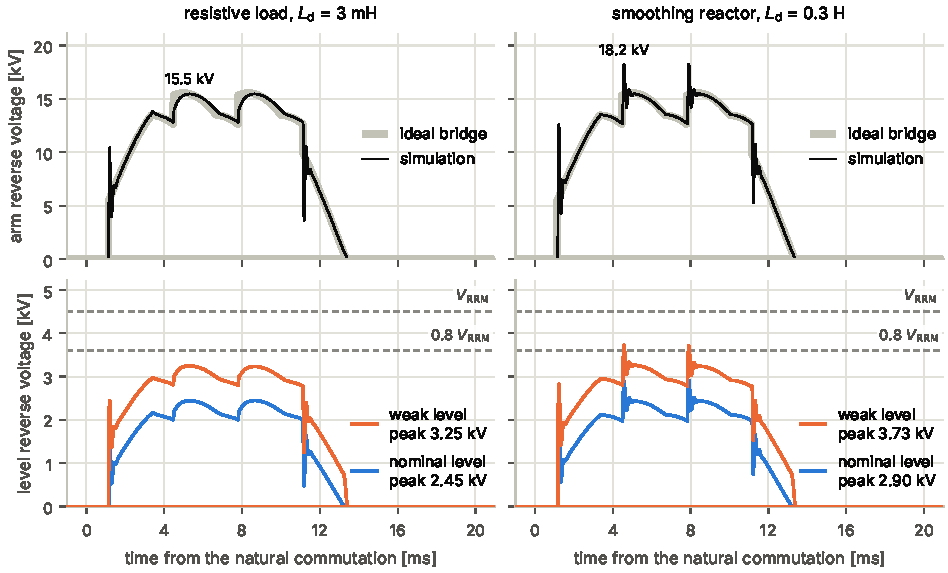
\includegraphics[width=\textwidth]{figures/fig_bridge_waveforms.pdf}
\caption{Reverse voltage of an arm (top) and of its weak level and one nominal level (bottom) over a period, grid at $+\dsKgrid\,\%$, design recovery set of Sec.~\ref{sec:recovery} with $u = \dsUunb$. Left: resistive load. Right: smoothing reactor.}
\label{fig:bridge}
\end{figure}

%=====================================================================
\section{Number of devices: first cut}
\label{sec:number}
The criterion is that the highest repetitive voltage of any level stays below a fraction $\ku$ of $\Vrrm$. An application note on RC snubbers for thyristors and diodes asks that the peak reverse voltage does not exceed \SI{80}{\percent} of the maximum blocking voltage of the device \cite[Sec.~4.4]{an6481}, so $\ku = 0.8$ is used here. Before any detailed calculation the number of devices follows from
\begin{equation}
n \;\ge\; \frac{\ktr\,\ksh\,\Vh_\mathrm{max}}{\ku\,\Vrrm},
\label{eq:n}
\end{equation}
where $\Vh_\mathrm{max}$ is the crest of the highest sustained line voltage and the two factors collect what the rest of the note computes:
\begin{itemize}
\item $\ktr = \Vs/\Vh$, the \emph{transient factor} of the arm: 1.0 when the DC side damps the commutation transient, 1.15 to 1.25 with a current-stiff DC side and a snubber of ordinary size, \eqref{eq:ktr};
\item $\ksh = \Vw/(\Vs/n)$, the \emph{sharing factor} of the weak level: it collects the charge difference at turn-off and the tolerance of the capacitors, \eqref{eq:vwtol}. Values of 1.25 to 1.35 are typical when the devices are matched in recovered charge; without matching it can exceed 1.5.
\end{itemize}
Three further points belong to this step. The non-repetitive rating $n\,\Vrsm$ has to be coordinated with the protection level of the surge arresters on the AC side. Press-pack diodes fail short, so the stack keeps conducting with one failed device; if the bridge has to stay in service in that state, the check is repeated with $n - 1$ (Sec.~\ref{sec:faults}). Finally, a larger $n$ lowers the level voltage but adds forward losses, levels and height: \eqref{eq:n} with a comfortable $\ksh$ is cheaper than a very tight specification of the devices.

\subsection{Worked example}
With $\Vh_\mathrm{max} = \SI{\dsVhatMax}{\kilo\volt}$ and $\ku\Vrrm = \SI{\dsKuVrrm}{\kilo\volt}$, the factors found in the following sections are $\ktr = \dsKtrR$, $\ksh = \dsKshR$ in case \caseR{} and $\ktr = \dsKtrL$, $\ksh = \dsKshL$ in case \caseL{}. Equation~\eqref{eq:n} gives $n \ge \dsNminR$ and $n \ge \dsNminL$: \dsNword{} devices are enough with the resistive load, while a current-stiff DC side asks for \dsNplusWord{}, or for a larger snubber (Sec.~\ref{sec:ex-transient}). The \dsNword{} diodes add up to $n\Vrrm = \SI{\dsNVrrm}{\kilo\volt}$, so the crest uses only \SI{\dsStackUtil}{\percent} of the series rating: the rest is taken by sharing and transients.

%=====================================================================
\section{Static sharing}
\label{sec:static}
\subsection{Leakage current}
A blocking diode behaves as a current sink: its leakage current depends weakly on the voltage and strongly on the temperature. The datasheet gives one number, the limit $\Irm$ at $\Vrrm$ and at the maximum junction temperature. The stack works at a fraction of $\Vrrm$ and at a lower temperature, where the leakage is one to two decades smaller. An application note on series connection gives two normalised curves for this scaling, against the blocking voltage and against the junction temperature \cite[Fig.~4]{an6531}, with the warning that they are approximate:
\begin{equation}
\Ilk(v, \Tj) \simeq \Irm\; k_v\!\left(\frac{v}{\Vrrm}\right) k_T(\Tj) .
\label{eq:ilk}
\end{equation}
The spread between devices is not specified. The worst case for the voltage of one level is a diode without leakage in a string of diodes at the limit, so the difference to design for is $\Delta\Ilk = \Ilk$.

\subsection{Balancing resistor}
With a constant voltage $V_\mathrm{s}$ on the string, each level carries the same current, and the diode without leakage takes the voltage
\begin{equation}
v_\mathrm{w} = \frac{V_\mathrm{s}}{n} + \frac{n-1}{n}\,\Rb\,\Delta\Ilk .
\label{eq:static}
\end{equation}
The application note \cite[Sec.~2.2.1]{an6531} gives two sizing rules. The simple one asks that the resistor carries two to five times the leakage current of the device at the working temperature and voltage. The refined one is the largest resistance that keeps the device voltage below $V_\mathrm{D}$,
\begin{equation}
\Rb \le \frac{n\,(1-a)\,V_\mathrm{D} - (1+a)(1+b)\,V_\mathrm{s}}{(n-1)(1-a^2)\,\Ilk},
\label{eq:an2}
\end{equation}
with $a$ the tolerance of the resistors, $b$ the tolerance of the string voltage and $\Ilk$ the maximum leakage current at the working temperature \cite[Eq.~(2)]{an6531}, which the note takes from \cite{williams}. The note defines $V_\mathrm{D}$ as the rated voltage of the device; with $V_\mathrm{D} = \ku\Vrrm$ the same relation keeps the design margin. Because the resistor dissipates, the note recommends the highest resistance that satisfies \eqref{eq:an2}. It also recommends to design with the datasheet limit of the leakage, or with the value at the expected temperature and voltage plus a margin when the losses matter \cite[Sec.~2.2.4]{an6531}.

\subsection{What the resistor does in a line-frequency bridge}
\label{sec:rbrole}
Relations \eqref{eq:static} and \eqref{eq:an2} describe a DC equilibrium. An arm of the bridge blocks for two thirds of a period and then conducts, and each level also has the capacitor $\Csn$. The equilibrium is reached with the time constant
\begin{equation}
\taus = \Rb\,\Csn ,
\end{equation}
to be compared with the blocking interval $2/(3f)$. If $\taus$ is longer than the blocking interval, which is the usual case, the levels share the voltage through their capacitors and the resistor only bends the result:
\begin{itemize}
\item a leakage difference acts as a current that charges $\Csn$: the offset of the level grows as $\tfrac{n-1}{n}\,\Delta\Ilk\,t/\Csn$ during the blocking interval and is reset by the next conduction;
\item an offset left by the turn-off (Sec.~\ref{sec:dynamic}) decays by the factor $e^{-t/\taus}$ only.
\end{itemize}
The resistor decides the sharing when the arm blocks for a long time: a bridge energised with the DC side open or held by another source, and the time after de-energisation, when $\Rb$ discharges the capacitors. This is the case the application note has in mind when it says that an RC snubber in parallel with each device is often sufficient in the off-state, and that a parallel resistor is highly recommended when a high DC voltage is applied for extended periods \cite[Sec.~2.2.1]{an6531}. For the running bridge, the consequence is that $\Rb$ is not a tool against the dynamic unbalance: halving it costs twice the losses and moves the peak of the weak level by a few percent.

\subsection{Ratings of the resistor}
The resistor sees the voltage of its level: the power is $V_\mathrm{rms}^2/\Rb$ with the rms voltage of the weak level, which is 1.3 to 1.5 times that of a nominal level. The element has to be rated for the repetitive peak of the level with the tolerances, for the impulse voltage of the level (Sec.~\ref{sec:insulation}) and for the power at the air temperature inside the stack. High-voltage thick-film resistors are the usual choice; their standard tolerance is often \SI{\pm10}{\percent}, and \eqref{eq:an2} shows what a tighter one is worth.

\subsection{Worked example}
At the crest of the highest grid voltage a balanced level blocks $\Vh/n = \SI{\dsVlev}{\kilo\volt}$, \SI{\dsStackUtil}{\percent} of $\Vrrm$. With the curves of App.~\ref{app:data}, a diode at the datasheet limit ($\Irm = \SI{\dsIrm}{\milli\ampere}$ at \SI{\dsTvjMax}{\celsius}) leaks \SI{\dsIlkDes}{\milli\ampere} at this voltage and at the design temperature $\Tj = \SI{\dsTjDes}{\celsius}$ (\SI{\dsIlkEightyFive}{\milli\ampere} at \SI{85}{\celsius}, \SI{\dsIlkHundredTwentyFive}{\milli\ampere} at \SI{125}{\celsius}). $\Rb = \SI{\dsRb}{\kilo\ohm}$ carries \SI{\dsIRb}{\milli\ampere}, \dsIlkRatio{} times the leakage: slightly above the range of the simple rule. Equation~\eqref{eq:an2} with $a = \SI{\dsTolRb}{\percent}$, $b = \SI{\dsKgrid}{\percent}$ and $V_\mathrm{s} = \sqrt2\,U$ gives
\begin{equation*}
\Rb \le \frac{\SI{\dsRbNumDes}{\volt}}{\Ilk} = \SI{\dsRbMaxDes}{\kilo\ohm} \ \ \text{for}\ V_\mathrm{D} = \ku\Vrrm, \qquad
\Rb \le \frac{\SI{\dsRbNumRated}{\volt}}{\Ilk} = \SI{\dsRbMaxRated}{\kilo\ohm} \ \ \text{for}\ V_\mathrm{D} = \Vrrm .
\end{equation*}
With \SI{\dsRb}{\kilo\ohm} the design voltage $\ku\Vrrm$ is kept up to a leakage of \SI{\dsIlkAdmDes}{\milli\ampere}, that is up to $\Tj = \SI{\dsTcovDes}{\celsius}$ for a diode at the limit, and the rated voltage up to \SI{\dsTcovRated}{\celsius}.

The time constant is $\taus = \SI{\dsTauB}{\milli\second}$ against a blocking interval of \SI{\dsTblock}{\milli\second}: \SI{\dsDecayBlock}{\percent} of an offset survives the interval, so the sharing of the running bridge is capacitive. The simulations confirm it. The leakage difference raises the peak of the weak level by \SI{\dsLeakTerm}{\volt} in the hand calculation; in the simulation of case \caseR{} the peak is \SI{\dsRVpkW}{\kilo\volt} with the worst leakage assignment, \SI{\dsRNoleakVpkW}{\kilo\volt} without any leakage and \SI{\dsRLeakwVpkW}{\kilo\volt} when the weak diode is the one that leaks. With $\Rb = \SI{\dsRbHalf}{\kilo\ohm}$ the peak falls to \SI{\dsRbHalfRVw}{\kilo\volt} and the resistor of the weak level dissipates \SI{\dsRbHalfRPw}{\watt} instead of \SI{\dsRPrbW}{\watt}; with \SI{\dsRbDouble}{\kilo\ohm} the peak is \SI{\dsRbDoubleRVw}{\kilo\volt} at \SI{\dsRbDoubleRPw}{\watt}. The value is therefore chosen on the static criterion and on the losses. At \SI{\dsRb}{\kilo\ohm} the weak level dissipates \SI{\dsRPrbW}{\watt} at \SI{\dsRVrmsW}{\kilo\volt} rms and a nominal level \SI{\dsRPrbN}{\watt} at \SI{\dsRVrmsN}{\kilo\volt} rms.

%=====================================================================
\section{Reverse recovery at the slope of the circuit}
\label{sec:recovery}
\subsection{The problem}
The dynamic sharing and the snubber losses depend on two numbers of the diode at turn-off, the recovered charge $\Qrr$ and the peak reverse current $\Irr$, and on how much they differ from device to device. A rectifier-diode datasheet gives them at one point, typically a forward current of about \SI{1}{\kilo\ampere} that falls at a few amperes per microsecond, at the maximum temperature, with a curve of the stored charge against the slope over one or two decades. The bridge works a decade or more below that range (Sec.~\ref{sec:bridge}). Two ways of extrapolating are at hand and they disagree by an order of magnitude:
\begin{itemize}
\item \emph{linear scaling} with the slope, which is what a charge-control model with a constant lifetime does;
\item \emph{continuing the power law} of the datasheet curve, $Q_\mathrm{S} \propto (di/dt)^m$ with $m$ of 0.25 to 0.5.
\end{itemize}
Both are wrong, in opposite directions, and the reason shows how to bound the result.

\subsection{Long ramp with a constant lifetime}
\label{sec:lm}
The charge-control model of Lauritzen and Ma \cite{lauritzen1991,ma1993} describes the diode with the charge $q_\mathrm{M}$ stored in the base, the charge $q_\mathrm{E}$ that the junction voltage would sustain, a lifetime $\tau$ and a transit time $\TM$:
\begin{equation}
\frac{dq_\mathrm{M}}{dt} = i - \frac{q_\mathrm{M}}{\tau}, \qquad i = \frac{q_\mathrm{E} - q_\mathrm{M}}{\TM} .
\label{eq:lm}
\end{equation}
While the diode conducts, the circuit imposes $i$. The junction blocks when $q_\mathrm{E}$ reaches zero; from then on $i = -q_\mathrm{M}/\TM$ and the current decays with the time constant $\trr$. On a ramp $i = -\alpha t$ that is long compared with $\tau$ the solution is closed:
\begin{equation}
\trr = \frac{\tau\,\TM}{\tau + \TM}, \qquad \ta = \tau - \trr, \qquad \Irr = \alpha\,\ta, \qquad \Qrr = \frac{\alpha}{2}\left(\tau^2 - \trr^2\right) = \Irr\left(\frac{\ta}{2} + \trr\right) .
\label{eq:longramp}
\end{equation}
Neither value depends on the forward current: the condition is $\Id/\alpha$ of several lifetimes, which the application note on snubbers states in the same way \cite[Sec.~2.1]{an6481}. Both values are proportional to the slope. Conversely, one pair $(\Qrr, \Irr)$ at a slope $a$ gives the parameters,
\begin{equation}
\trr = \frac{\Qrr}{\Irr} - \frac{\Irr}{2a}, \qquad \tau = \trr + \frac{\Irr}{a}, \qquad \TM = \frac{\tau\,\trr\,a}{\Irr} ,
\label{eq:lmfit}
\end{equation}
where the first relation is the one given in \cite[Eq.~(2)]{an6481} for the time constant of an exponential tail. The softness of the recovery is described here by $s = 2\trr/\ta$, the ratio of the two times of a triangle with the same charge, so that $\Qrr = \Irr^2 (1+s)/(2\alpha)$.

\subsection{Why the datasheet point cannot be scaled}
Relations \eqref{eq:longramp} say that the stored charge of a diode with a constant lifetime is proportional to the slope, exponent 1. Datasheet curves are much flatter. The flatness comes from recombination that grows faster than the charge at high carrier density, in the end regions and by the Auger process \cite{schlangenotto1969,schlangenotto1972}: at the datasheet point the effective lifetime is short, at the slope of the bridge the density is low and the long bulk lifetime $\taub$ takes over. A quadratic term added to \eqref{eq:lm} reproduces this,
\begin{equation}
\frac{dq_\mathrm{M}}{dt} = i - \frac{q_\mathrm{M}}{\taub} - k\,q_\mathrm{M}^2 ,
\label{eq:quad}
\end{equation}
and it has two limits on a ramp. When the linear term dominates, the charge at the current zero is $\alpha\taub^2$, exponent 1. When the quadratic term dominates, the equation has no time constant and the charge scales as $(\alpha/k^2)^{1/3}$, exponent $1/3$. The exponent of the datasheet curve therefore tells which regime the test point is in. An exponent of 0.25 to 0.5 means that the test point is dominated by the quadratic term, and that the curve carries almost no information on $\taub$, which is the parameter that sets the charge in the bridge.

The model \eqref{eq:quad} has three parameters, $\taub$, $\TM$ and $k$, and the datasheet gives two numbers and a slope. The fit is therefore a family: for each assumed $\taub$, the pair $(\TM, k)$ is found that reproduces the table values of $Q_\mathrm{S}$ and $\Irr$ and the local slope of the $Q_\mathrm{S}$ curve, and the model is then evaluated on the ramp of the circuit. The family has two ends, which bound the result, and two intermediate members are useful:
\begin{itemize}
\item \emph{floor}: $k = 0$, the constant-lifetime model through the table point, \eqref{eq:lmfit}. It is the linear scaling and gives the smallest charge;
\item \emph{ceiling}: no bulk recombination at all, $\taub \to \infty$. It gives the largest charge that is compatible with the datasheet;
\item \emph{central}: the bulk lifetime of the device family, when a complete set of curves is available for a similar device;
\item \emph{upper}: a long bulk lifetime, taken as the upper end of what the family can deliver.
\end{itemize}
The power-law continuation of the datasheet curve lies above the ceiling: it is not a member of the family and overestimates the charge.

\subsection{Temperature, spread and matching}
Lifetimes grow with temperature \cite{lutz}. With $\tau \propto T$ (absolute temperature) the long-ramp values scale as $\Qrr \propto T^2$ and $\Irr \propto T$; this exponent is an assumption on the low side, so the values at a design temperature below the datasheet temperature are on the safe side.

The spread between devices is mainly a spread of lifetime. Its effect on the charge depends on the regime: the logarithmic sensitivity $\partial\ln\Qrr/\partial\ln\taub$ is close to 2 where the bulk lifetime dominates and much smaller at the datasheet point. A band of $Q_\mathrm{S}$ measured at the datasheet conditions is therefore \emph{wider} at the slope of the bridge, by the ratio of the two sensitivities. The application note states that $Q_\mathrm{S}$ has the most significant impact on series connections and should be carefully matched, that it is not measured routinely and that it is provided, like the banding on $Q_\mathrm{S}$, on request \cite[Sec.~2.2.3]{an6531}. Two things should be asked together with the devices: the values of $Q_\mathrm{S}$ and $\Irr$ at the slope of the circuit, or at the lowest slope the manufacturer can test, and the band at that slope.

When the data are not available, the charge can be measured on a bench with a half-sine current pulse from a capacitor through an inductor: a pulse of angular frequency $\omega_\mathrm{t}$ and amplitude $I_\mathrm{p}$ crosses zero with the slope $\omega_\mathrm{t} I_\mathrm{p}$, and its length has to be several lifetimes. A slope of \SI{0.2}{\ampere\per\micro\second} with \SI{100}{\ampere} needs a half period of about \SI{1.6}{\milli\second}. The reverse current and its integral are recorded at the design temperature on several devices.

\subsection{In the bridge the ramp is not straight}
The commutation voltage is sinusoidal, so the slope of the arm current grows during the overlap and reaches $\alpha$ at the end. The stored charge follows a slope that was smaller: with the second derivative of the current, $\alpha\,\omega\cot\mu$, the charge at the current zero is lower than on a straight ramp by the factor
\begin{equation}
1 - \omega\,\tau\cot\mu .
\label{eq:rampcorr}
\end{equation}
The correction is a few percent and the long-ramp values \eqref{eq:longramp} are on the safe side.

\subsection{Worked example}
\label{sec:ex-recovery}
The assumed datasheet of the diode (App.~\ref{app:data}) gives $Q_\mathrm{S} = \SI{\dsQsTab}{\micro\coulomb}$ and $\Irr = \SI{\dsIrrTab}{\ampere}$ at \SI{\dsIfTab}{\ampere}, \SI{\dsATab}{\ampere\per\micro\second} and \SI{\dsTTab}{\celsius}, and a curve of $Q_\mathrm{S}$ with exponent \dsQsSlope{} between \dsAQsLo{} and \SI{\dsAQsHi}{\ampere\per\micro\second}. The bridge commutates at \SI{\dsAlphaNom}{\ampere\per\micro\second} at the rated point. At \SI{\dsTTab}{\celsius}, linear scaling of the table point gives \SI{\dsQlinTab}{\micro\coulomb}; the power law gives \SI{\dsQpowTab}{\micro\coulomb}.

For the central scenario the bulk lifetime is taken from a device of the same voltage class for which complete curves are published: the three-parameter model was fitted to the curves of $Q_\mathrm{S}$ and $\Irr$ between 1 and \SI{30}{\ampere\per\micro\second} of a \SI{4.2}{\kilo\volt} thyristor \cite[Figs.~12 and~13]{an5950}. The fit gives a bulk lifetime of \SI{\dsClsTauMax}{\micro\second} at \SI{125}{\celsius} on the maximum curves and \SI{\dsClsTauMin}{\micro\second} on the minimum curves, with an rms error of \SI{\dsClsRmsMax}{\percent}. On those curves the power law overestimates the charge at \SI{0.1}{\ampere\per\micro\second} by a factor of \dsClsQratioMax{} (\SI{\dsClsQlawMax}{\micro\coulomb} against \SI{\dsClsQMax}{\micro\coulomb} of the model). The longer value, brought to \SI{\dsTTab}{\celsius}, is the central lifetime of \SI{\dsTauClass}{\micro\second}. It belongs to another device and is an indication only; this is why the upper scenario with \SI{\dsTauUpper}{\micro\second} and the two bounds are carried along.

\begin{table}[htb]
\centering\small
\caption{Scenarios of the bulk lifetime: parameters of \eqref{eq:quad} fitted on the datasheet point, and recovery at the rated operating point (\SI{\dsAlphaNom}{\ampere\per\micro\second}). The last two columns are the deviation of the model from the datasheet curve at its two ends.}
\label{tab:scen}
\begin{tabular}{@{}lccccccccccc@{}}
\toprule
 & $\taub$ & $\TM$ & $k$ & \multicolumn{2}{c}{at \SI{\dsTTab}{\celsius}} & \multicolumn{2}{c}{at \SI{\dsTjDes}{\celsius}} & $s$ & \multicolumn{2}{c}{curve ends} \\
\cmidrule(lr){5-6}\cmidrule(lr){7-8}\cmidrule(l){10-11}
Scenario & [\si{\micro\second}] & [\si{\micro\second}] & [$10^{-6}/(\si{\micro\coulomb\,\micro\second})$] & $\Qrr$ [\si{\micro\coulomb}] & $\Irr$ [A] & $\Qrr$ [\si{\micro\coulomb}] & $\Irr$ [A] & & low & high \\
\midrule
floor & \dsTauFloor & \dsTmFloor & 0 & \dsQhotFloorNom & \dsIhotFloorNom & \dsQFloorNom & \dsIFloorNom & \dsSoftFloor & $\dsDevLoFloor\,\%$ & $+\dsDevHiFloor\,\%$ \\
central & \dsTauClass & \dsTmCentral & \dsKCentral & \dsQhotCentralNom & \dsIhotCentralNom & \dsQCentralNom & \dsICentralNom & \dsSoftCentral & $\dsDevLoCentral\,\%$ & $+\dsDevHiCentral\,\%$ \\
upper & \dsTauUpper & \dsTmUpper & \dsKUpper & \dsQhotUpperNom & \dsIhotUpperNom & \dsQUpperNom & \dsIUpperNom & \dsSoftUpper & $\dsDevLoUpper\,\%$ & $+\dsDevHiUpper\,\%$ \\
ceiling & $\infty$ & \dsTmCeiling & \dsKCeiling & \dsQhotCeilingNom & \dsIhotCeilingNom & \dsQCeilingNom & \dsICeilingNom & \dsSoftCeiling & $\dsDevLoCeiling\,\%$ & $+\dsDevHiCeiling\,\%$ \\
\bottomrule
\end{tabular}
\end{table}

\begin{figure}[htb]
\centering
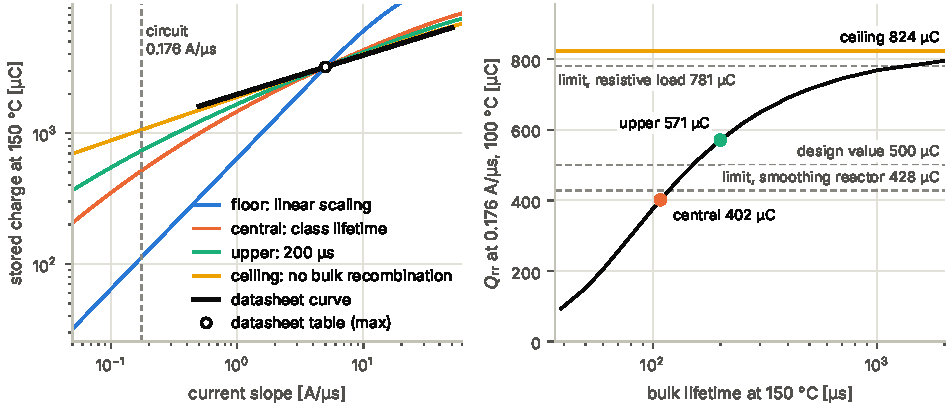
\includegraphics[width=\textwidth]{figures/fig_recovery_slope.pdf}
\caption{Left: stored charge against the current slope at \SI{\dsTTab}{\celsius} for the four scenarios, all through the datasheet point. Right: recovered charge at the slope of the bridge and at \SI{\dsTjDes}{\celsius} against the assumed bulk lifetime, with the design value and the limits of Sec.~\ref{sec:ex-dynamic}.}
\label{fig:recovery}
\end{figure}

Table~\ref{tab:scen} and Fig.~\ref{fig:recovery} show the result. All four members pass through the table point; the floor misses the slope of the datasheet curve completely, the ceiling follows it best. At the slope of the bridge the charge spans one decade, from \SI{\dsQFloorNom}{\micro\coulomb} to \SI{\dsQCeilingNom}{\micro\coulomb} at \SI{\dsTjDes}{\celsius}, and the peak reverse current goes from \SI{\dsIFloorNom}{\ampere} to \SI{\dsICeilingNom}{\ampere}. From \SI{\dsTTab}{\celsius} to \SI{\dsTjDes}{\celsius} the charge falls by the factor \dsFacQ{} and the current by \dsFacI{}. The time scale changes as well: with the quadratic term the peak comes \SIrange{\dsTaCentral}{\dsTaCeiling}{\micro\second} after the current zero, against \SI{\dsTaTab}{\micro\second} at the datasheet point, while the tail keeps a time constant close to $\TM$, so the softness $s$ falls from \dsSoftTab{} to \dsSoftCeiling{}--\dsSoftCentral{}.

The sensitivity of the charge to the bulk lifetime in the central scenario is \dsSensWp{} at the slope of the bridge and \dsSensDs{} at the datasheet point: a band of \SI{10}{\percent} on the datasheet $Q_\mathrm{S}$ is a band of \SI{\dsBandTen}{\percent} in the bridge.

The network of the example is designed with the set
\begin{equation*}
\Qrr = \SI{\dsQdes}{\micro\coulomb}, \quad \Irr = \SI{\dsIdes}{\ampere} \quad \text{at}\ \SI{\dsAref}{\ampere\per\micro\second},\ \SI{\dsTjDes}{\celsius}, \qquad u = \dsUunb ,
\end{equation*}
which lies between the central and the upper scenario and takes the unbalance from a \SI{10}{\percent} band widened by the factor above. Relations \eqref{eq:lmfit} turn it into $\tau = \SI{\dsLmTau}{\micro\second}$, $\TM = \SI{\dsLmTm}{\micro\second}$, $\trr = \SI{\dsLmTt}{\micro\second}$, $\ta = \SI{\dsLmTa}{\micro\second}$ ($s = \dsSdes$) for the nominal diodes; the weak diode has the charge $\Qrr(1-u)$ and the current $\Irr\sqrt{1-u}$, that is the same softness. At the slope of the grid at $+\dsKgrid\,\%$ the same diode gives \SI{\dsQlmAtMax}{\micro\coulomb} and \SI{\dsIlmAtMax}{\ampere}, at $\uk = \dsUkMin\,\%$ \SI{\dsQlmAtUkmin}{\micro\coulomb} and \SI{\dsIlmAtUkmin}{\ampere}. The correction \eqref{eq:rampcorr} is \SI{\dsRampCorr}{\percent}; in the simulation of the balanced stack the recovered charge is \SI{\dsRBalQrrN}{\micro\coulomb} and the peak \SI{\dsRBalIrrmN}{\ampere}.

%=====================================================================
\section{Dynamic sharing}
\label{sec:dynamic}
\subsection{Mechanism}
At turn-off the $n$ diodes of the arm carry the same current. Each one conducts in reverse until its stored charge is used up. The diode with the smallest charge, the weak one, reaches its peak reverse current first and blocks; from that instant the current of the string flows through its snubber while the other diodes still conduct (Fig.~\ref{fig:turnoff}). When the other diodes block as well, the capacitor of the weak level has received a charge that the others have not: the difference of the recovered charges,
\begin{equation}
\Delta Q = \Qrr - \Qrr(1-u) = u\,\Qrr ,
\end{equation}
which is the relation $\Delta V \approx \Delta Q_\mathrm{s}/C_\mathrm{s}$ of the application note \cite[Eq.~(1)]{an6531}. After that the string current is common to all levels, every capacitor receives the same charge and the offset stays. It decays only through $\Rb$, with $\taus$, and it is cancelled when the arm conducts again. There is no accumulation from cycle to cycle.

\begin{figure}[htb]
\centering
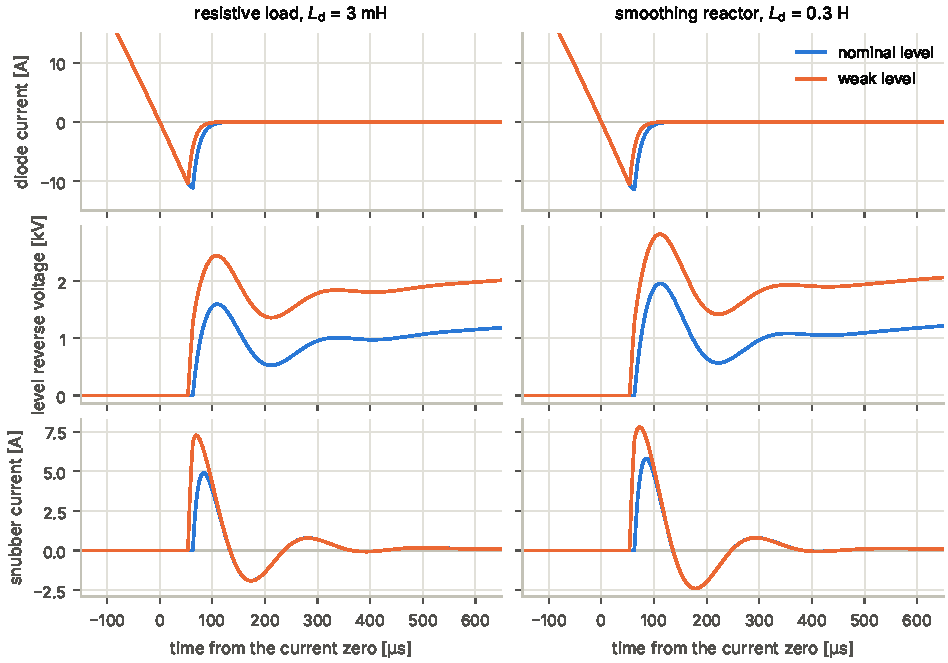
\includegraphics[width=\textwidth]{figures/fig_turn_off.pdf}
\caption{Turn-off of an arm of the worked example: diode currents, level voltages and snubber currents of the weak level and of a nominal level. The weak diode blocks about \SI{\dsTaDiff}{\micro\second} earlier and its snubber takes the string current alone during that time.}
\label{fig:turnoff}
\end{figure}

\subsection{Charge model of the weak level}
With equal capacitors that share the arm voltage $v_\mathrm{s}(t)$, and one of them carrying the extra charge, the weak level follows
\begin{equation}
v_\mathrm{w}(t) = \frac{v_\mathrm{s}(t)}{n} + \frac{n-1}{n}\,\Delta v(t), \qquad
\Delta v(t) = \frac{\Delta Q}{\Csn}\,e^{-t/\taus} + \Rb\,\Delta\Ilk\left(1 - e^{-t/\taus}\right),
\label{eq:vw}
\end{equation}
with $t$ counted from the turn-off. The second term of $\Delta v$ is the leakage difference of Sec.~\ref{sec:static}. The offset is the same at every instant of the blocking interval, apart from the slow decay, so the weak level peaks when the arm does. If in addition the capacitor of the weak level is at the lower end of its tolerance, $\Csn(1-c)$, and the others at the upper end, $\Csn(1+c)$, the peak becomes
\begin{equation}
\Vw = \frac{(1+c)\,\Vs + (n-1)\,\Delta v(t_\mathrm{pk})}{n - (n-2)\,c} ,
\label{eq:vwtol}
\end{equation}
where $\Vs$ is the highest arm voltage and $t_\mathrm{pk}$ the time at which it occurs: $(\pi/2 - \mu)/\omega$ in case \caseR{}, where the arm peaks at the crest of the line voltage, and about $\pi/(3\omega)$ in case \caseL{}, where it peaks at the first step near the crest. The sharing factor of \eqref{eq:n} is $\ksh = n\Vw/\Vs$.

Solved for the capacitor, \eqref{eq:vwtol} gives the smallest value that keeps the weak level below $\ku\Vrrm$,
\begin{equation}
\Csn \ge \frac{(n-1)\,\Delta q}{\left[n - (n-2)c\right]\ku\Vrrm - (1+c)\,\Vs}, \qquad \Delta q = \Csn\,\Delta v(t_\mathrm{pk}) \simeq \Delta Q\,e^{-t_\mathrm{pk}/\taus} .
\label{eq:csn}
\end{equation}
The denominator is the margin that the arm voltage leaves. When it is small, no capacitor of reasonable size helps: either $n$ grows or $\Vs$ has to come down (Sec.~\ref{sec:transient}).

\subsection{Comparison with the application note}
The conservative relation of the application note for the smallest snubber capacitor is
\begin{equation}
C_\mathrm{s} \ge \frac{(n-1)\,\Delta Q_\mathrm{s}}{(1-c)\left(n\,V_\mathrm{D} - (1+b)\,V_\mathrm{s}\right)}
\label{eq:an3}
\end{equation}
\cite[Eq.~(3)]{an6531}. It is the same charge model with three simplifications. The capacitor tolerance is applied to the offset only; in \eqref{eq:vwtol} it also raises the share of the weak level in the arm voltage, from $1/n$ to $(1+c)/(n - (n-2)c)$, that is by about $(2 - 2/n)\,c$. The string voltage $V_\mathrm{s}$ carries a tolerance $b$ but no transient factor. The decay of the offset and the leakage difference are neglected; they act in opposite directions and in the example the decay is the larger of the two, so the net effect is on the safe side. The first two points go in the unsafe direction and the first one is not small: with $n = \dsN$ and $c = \SI{\dsTolC}{\percent}$ the share grows by \SI{\dsCapShareRel}{\percent}. The note also reminds that the first task of the capacitor is to limit the voltage at turn-off, that the RC snubber should be designed for that task first and then checked against \eqref{eq:an3}, and that a larger capacitor means more losses \cite[Sec.~2.2.3]{an6531}.

\subsection{Sensitivity to the recovered charge}
The offset is proportional to $\Delta Q = u\,\Qrr$, with a slope of $\tfrac{n-1}{n}\,e^{-t_\mathrm{pk}/\taus}/\Csn$ volts per coulomb. The two uncertain quantities of Sec.~\ref{sec:recovery}, the charge at the slope of the circuit and its spread, enter as a product. A design is robust when it states the charge difference it tolerates and that number is then asked from the manufacturer; it is fragile when it relies on a charge scaled from the datasheet point.

\subsection{Worked example}
\label{sec:ex-dynamic}
With the design set at the slope of the grid at $+\dsKgrid\,\%$ the charge difference is $\Delta Q = \dsUunb \times \SI{\dsQrrHand}{\micro\coulomb} = \SI{\dsDqHand}{\micro\coulomb}$, that is $\Delta Q/\Csn = \SI{\dsDvHand}{\kilo\volt}$. In case \caseR{} the arm peaks \SI{\dsTpkR}{\milli\second} after the turn-off, when \dsDecayR{} of the offset is left, and \eqref{eq:vw} gives
\begin{equation*}
\Vw = \frac{\SI{\dsHandRVs}{\kilo\volt}}{\dsN} + \frac{\dsNminus}{\dsN}\left(\dsDecayR \times \SI{\dsDvHand}{\kilo\volt} + \text{leakage term}\right) = \SI{\dsHandRVw}{\kilo\volt},
\end{equation*}
\SI{\dsHandRVwNoLk}{\kilo\volt} without the leakage term. With a capacitor tolerance of \SI{\pm\dsTolC}{\percent}, \eqref{eq:vwtol} gives \SI{\dsHandRVwTol}{\kilo\volt}. The simulation gives \SI{\dsRVpkW}{\kilo\volt} and \SI{\dsRCtolVpkW}{\kilo\volt}; adding the tolerance of $\Rb$ in the worst direction it gives \SI{\dsRTolVpkW}{\kilo\volt}, \SI{\dsRTolUtilW}{\percent} of $\Vrrm$. The hand values are \SI{\dsHandRDevVw}{\percent} and \SI{\dsHandRDevTol}{\percent} high, mainly because the simulated charge difference is \SI{\dsRDq}{\micro\coulomb}: the ramp is not straight \eqref{eq:rampcorr} and the nominal diodes recover a little less once the weak level has started to block. Equation~\eqref{eq:csn} asks for $\Csn \ge \SI{\dsCsnMinHandR}{\nano\farad}$ in case \caseR{}, which is how the \SI{\dsCsn}{\nano\farad} of the example were chosen; \eqref{eq:an3} with $V_\mathrm{D} = \ku\Vrrm$ asks for \SI{\dsCsMinDes}{\nano\farad} only, because it applies the tolerance to the offset and not to the share. Case \caseL{} needs the arm voltage of the next section.

\begin{figure}[htb]
\centering
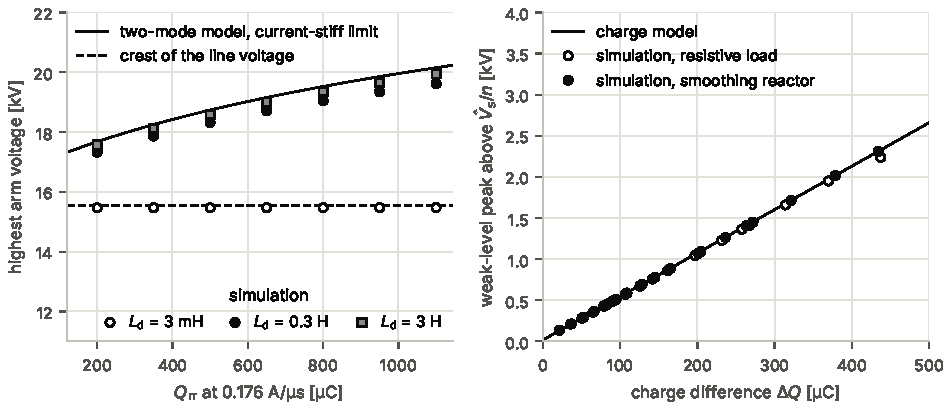
\includegraphics[width=\textwidth]{figures/fig_dynamic_sharing.pdf}
\caption{Check of the two hand models against the simulation. Left: highest arm voltage against the recovered charge of a balanced stack, for three values of the DC inductance, with the crest of the line voltage and the two-mode model of Sec.~\ref{sec:transient}. Right: offset of the weak level against the simulated charge difference, for $u$ of \dsUswList{}, with the charge model \eqref{eq:vw}.}
\label{fig:sharing}
\end{figure}

Figure~\ref{fig:sharing} (right) checks the structure of the model over the whole range: when the simulated arm peak and charge difference are put into \eqref{eq:vw}, the peak of the weak level is reproduced within \SI{\dsChargeDevLoR}{\percent} and $+\SI{\dsChargeDevHiR}{\percent}$ in case \caseR{} and within \SI{\dsChargeDevLoL}{\percent} and $+\SI{\dsChargeDevHiL}{\percent}$ in case \caseL{}, for charges from \dsQswLo{} to \SI{\dsQswHi}{\micro\coulomb} and unbalances up to \dsUswHi{}.

\begin{table}[htb]
\centering\small
\caption{Simulated peak of the weak level [kV] against the recovered charge (reference value at \SI{\dsAref}{\ampere\per\micro\second}, constant softness) and the unbalance $u$, with the power of its snubber resistor [W] for $u = \dsUunb$. Nominal network, grid at $+\dsKgrid\,\%$.}
\label{tab:qsweep}
\begin{tabular}{@{}cc|cccc|cccc@{}}
\toprule
 & & \multicolumn{4}{c|}{\caseR{} resistive load} & \multicolumn{4}{c}{\caseL{} smoothing reactor} \\
$\Qrr$ [\si{\micro\coulomb}] & $\Irr$ [A] & \dsQsweepHead{} & $P_{\Rsn}$ & \dsQsweepHead{} & $P_{\Rsn}$ \\
\midrule
\dsQsweepRows
\bottomrule
\end{tabular}
\end{table}

\begin{figure}[htb]
\centering
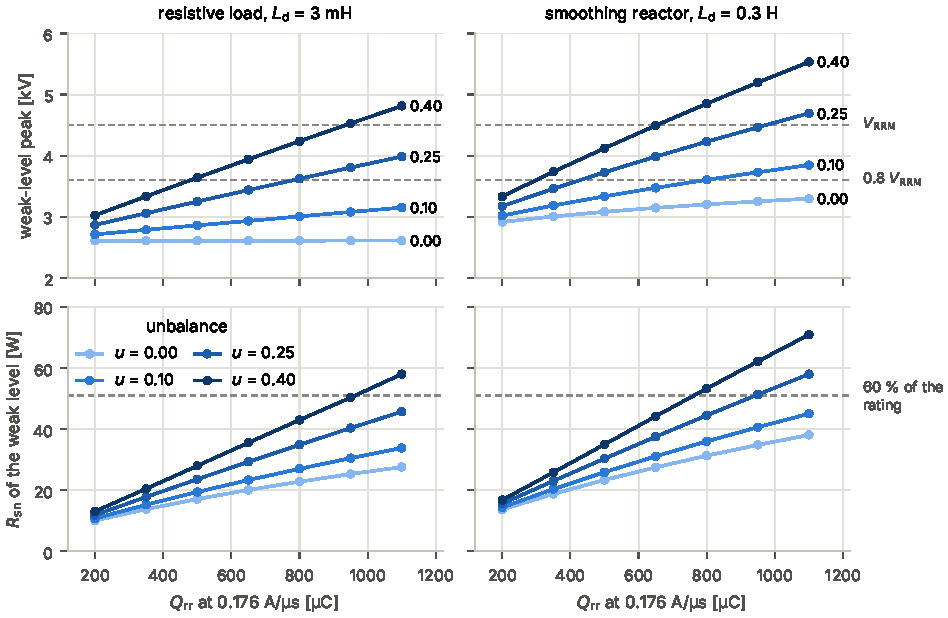
\includegraphics[width=\textwidth]{figures/fig_qrr_sensitivity.pdf}
\caption{Peak of the weak level and power of its snubber resistor against the recovered charge, for four values of the unbalance. The dashed lines are $\ku\Vrrm$, $\Vrrm$ and \SI{\dsKp}{\percent} of the rating of the resistor of the example at the air temperature of the stack (Sec.~\ref{sec:thermal}).}
\label{fig:qrr}
\end{figure}

Table~\ref{tab:qsweep} and Fig.~\ref{fig:qrr} give the sensitivity for the nominal network. With $u = \dsUunb$ the weak level reaches $\ku\Vrrm$ at $\Qrr = \SI{\dsQlimVR}{\micro\coulomb}$ in case \caseR{} and at \SI{\dsQlimVL}{\micro\coulomb} in case \caseL{} (Fig.~\ref{fig:recovery}, right); with the capacitor tolerance of \SI{\pm\dsTolC}{\percent} the two limits fall to \SI{\dsQlimVTolR}{\micro\coulomb} and \SI{\dsQlimVTolL}{\micro\coulomb}. The stack with the resistive load therefore covers the upper scenario (\SI{\dsQUpperNom}{\micro\coulomb}) with the tolerance, but not the ceiling (\SI{\dsQCeilingNom}{\micro\coulomb}). With the smoothing reactor the limit lies just above the central scenario (\SI{\dsQCentralNom}{\micro\coulomb}) without the tolerance and below it with the tolerance, in both cases below the design set; the next section shows why. At the design charge and without the tolerance, the unbalance that reaches $\ku\Vrrm$ is \dsUlimDesR{} in case \caseR{} and \dsUlimDesL{} in case \caseL{}.

%=====================================================================
\section{Commutation transient and snubber}
\label{sec:transient}
\subsection{One loop with a recovering diode}
\label{sec:oneloop}
The building block is a loop with a voltage step $W$ behind an inductance $L$ and a diode with a snubber $R$--$C$. At $t = 0$ the diode is at its peak reverse current $I$, which also flows in $L$; then the diode current decays as $I e^{-t/\trr}$ and the rest of the loop current goes into the snubber. With
\begin{equation}
\omega_0 = \frac{1}{\sqrt{LC}}, \qquad Z_0 = \sqrt{\frac{L}{C}}, \qquad \zeta = \frac{R}{2Z_0}, \qquad \chi = \frac{I\,Z_0}{W}, \qquad \vartheta = \omega_0\,\trr ,
\label{eq:norm}
\end{equation}
the capacitor voltage $y = v_C/W$ over the normalised time $x = \omega_0 t$ obeys
\begin{equation}
y'' + 2\zeta y' + y = 1 + \frac{\chi}{\vartheta}\,e^{-x/\vartheta}, \qquad y(0) = y'(0) = 0 ,
\label{eq:ode}
\end{equation}
and the voltage across the diode is $v = W f(x)$ with $f = y + 2\zeta y'$. The solution is
\begin{equation}
y = 1 + K e^{-x/\vartheta} + e^{-\zeta x}\left(A\cos\omega_\mathrm{d}x + B\sin\omega_\mathrm{d}x\right), \quad
K = \frac{\chi\,\vartheta}{1 - 2\zeta\vartheta + \vartheta^2}, \quad A = -(1+K), \quad B = \frac{\zeta A + K/\vartheta}{\omega_\mathrm{d}},
\label{eq:sol}
\end{equation}
with $\omega_\mathrm{d} = \sqrt{1-\zeta^2}$. The peak factor $F(\zeta,\chi,\vartheta) = \max f$ is listed in Table~\ref{tab:F}. For $\vartheta \to 0$ the diode snaps off, the forcing term becomes an impulse ($y'(0) = \chi$) and the solution is the classical one of McMurray \cite{mcmurray1972}, with an initial step $R\,I$ of the diode voltage. $\chi$ measures the energy in the inductance against the energy of the step: for $\chi > 1$ the transient is dominated by the reverse current. Snubber design with a realistic recovery waveform instead of the snap-off is the subject of \cite{chokhawala1991}.

\begin{table}[htb]
\centering\small
\caption{Peak factor $F$ of the diode voltage in the loop of Sec.~\ref{sec:oneloop}, for an ideal snap-off and for a tail with $\vartheta = 0.4$.}
\label{tab:F}
\begin{tabular}{@{}c|ccccc|ccccc@{}}
\toprule
 & \multicolumn{5}{c|}{$\vartheta = 0$ (snap-off)} & \multicolumn{5}{c}{$\vartheta = 0.4$} \\
$\zeta$ & $\chi = 0.5$ & 1.0 & 1.5 & 2.0 & 3.0 & $\chi = 0.5$ & 1.0 & 1.5 & 2.0 & 3.0 \\
\midrule
\dsFtabRows
\bottomrule
\end{tabular}
\end{table}

Two properties of $F$ matter for a stack. For a given $\chi$ the peak has a flat minimum in $\zeta$: near $\zeta = 0.4$ to 0.5 for $\chi$ between 1.5 and 3, at a heavier damping for smaller $\chi$. A soft tail removes the initial step $R\,I$. With a light damping ($\zeta$ up to about 0.4) it nevertheless raises the peak, by up to \SI{10}{\percent}, because the inductance keeps charging while the diode still conducts; with a heavy damping it lowers the peak, which for the snap-off is then the initial step itself.

\subsection{The bridge: two modes}
\label{sec:modes}
In the bridge the loop is not single. Take the turn-off of arm a$+$ at the end of the commutation from phase a to phase b, while c$-$ conducts. The two conducting arms tie the DC terminals to b and c, and the four blocking arms are four snubber strings, each $\Zs = \Rs + 1/(s\Cs)$ with $\Rs = n\Rsn$ and $\Cs = \Csn/n$: the arm that has just turned off between a and b, the other arm of its phase (a$-$) between a and c, and two arms (b$-$ and c$+$) in parallel between b and c, that is across the DC terminals. Behind each AC terminal sits $\Lc$. With a current-stiff DC side this network has two modes (App.~\ref{app:modes}),
\begin{equation}
\text{mode 1: phase a against b and c,}\quad \Zs + 3s\Lc = 0; \qquad
\text{mode 2: b against c,}\quad \Zs + 5s\Lc = 0 ,
\end{equation}
and each of them is a loop of the kind of Sec.~\ref{sec:oneloop}. With $m_1 = 3$ and $m_2 = 5$ the normalised quantities of mode $k$ are
\begin{equation}
\omega_{0k} = \frac{1}{\sqrt{m_k\Lc\Cs}}, \quad Z_{0k} = \sqrt{\frac{\Lc}{m_k\Cs}}, \quad \zeta_k = \frac{\Rs}{2\,m_k Z_{0k}}, \quad \chi_k = \frac{2\,\Irr Z_{0k}}{\Vos}, \quad \vartheta_k = \omega_{0k}\,\trr ,
\label{eq:modes}
\end{equation}
and $f_k(t) = f(\omega_{0k}t;\,\zeta_k,\chi_k,\vartheta_k)$. The step that excites them is the commutation voltage at the instant of the peak reverse current, which comes $\ta$ after the end of the ideal overlap:
\begin{equation}
\Vos = \Vh\sin(\mu + \omega\ta), \qquad \ta = \Irr/\alpha .
\label{eq:V0s}
\end{equation}
Mode~1 takes the step $\tfrac34\Vos$ and the whole reverse current, mode~2 the step $\tfrac12\Vos$ and half the current. The arm voltages after the turn-off are the ideal waveform $v_\mathrm{id}$ of \eqref{eq:varm} plus the modal transients:
\begin{align}
\text{arm that turns off:}\quad & v = \Vos\left(\tfrac34 f_1 + \tfrac14 f_2\right), \label{eq:vown}\\
\text{arms across the DC terminals:}\quad & v = v_\mathrm{id} + \tfrac12\Vos\,(f_2 - 1), \label{eq:vdcarm}\\
\text{other arm of the same phase:}\quad & v = v_\mathrm{id} + \Vos\left[\tfrac34(1 - f_1) - \tfrac14(1 - f_2)\right]. \label{eq:vother}
\end{align}
The arm that turns off starts from zero and stays far below the crest. The arms across the DC terminals are the ones that receive the steps of $+\Vo/2$ of \eqref{eq:steps} near the crest, and \eqref{eq:vdcarm} is the overshoot of those steps. The highest arm voltage and the transient factor of \eqref{eq:n} are therefore
\begin{equation}
\Vs \simeq \Vh + \tfrac12\Vos\,(F_2 - 1), \qquad \ktr \simeq 1 + \tfrac12\sin(\mu + \omega\ta)\,(F_2 - 1) ,
\label{eq:ktr}
\end{equation}
with $F_2$ the peak factor of mode~2. This is the point where a stack differs from a single device: a snubber design that looks at the device that turns off does not see the highest voltage. The application note on snubbers reduces the bridge to one loop for the arm that turns off, with the equivalent values $R_\mathrm{eq} = \tfrac35\Rs$ and $C_\mathrm{eq} = \tfrac53\Cs$ in a loop of $2\Lc$ \cite[Sec.~4.2]{an6481}. This is the impedance seen by that arm, $\Zs$ in parallel with $\Zs + \Zs/2$; it predicts the peak of that arm within a few percent (Table~\ref{tab:modeval}), and says nothing on the other three.

\subsection{Role of the DC side}
\label{sec:dcrole}
Mode~2 runs between the DC terminals. Its loop has the inductance $2\Lc$ and the characteristic impedance $2Z_{02}$, and whatever is connected to the DC terminals is in parallel with its snubber branch. A DC side whose impedance at $\omega_{02}$ is much larger than $2Z_{02}$ does not take part; for a reactor this means
\begin{equation}
\omega_{02}\Ld \gg 2Z_{02} \quad\Longleftrightarrow\quad \Ld \gg 2\Lc .
\label{eq:stiff}
\end{equation}
A load resistance of the order of $2Z_{02}$ or less, with little inductance in series, damps mode~2: the terms with $f_2$ vanish from \eqref{eq:vown}--\eqref{eq:vother}, the arms across the DC terminals follow the ideal waveform and $\ktr = 1$. Between the two limits the result has to be simulated with the real load, including cables and filters, whose impedance at a few kilohertz is rarely the one at DC.

\subsection{Choice of the capacitor and of the resistor}
\label{sec:rsnchoice}
The capacitor acts twice. It divides the charge difference, \eqref{eq:csn}, and it lowers $Z_{0k}$ and with it $\chi_k$ and the overshoot. Its cost is the loss of the resistor, which has a term proportional to $\Csn$ (Sec.~\ref{sec:prsn}), and the size of a high-voltage film capacitor.

The resistor sets the damping. From \eqref{eq:modes}, $\zeta_2 = \tfrac12\Rsn\sqrt{n\Csn/(5\Lc)}$, and the highest arm voltage \eqref{eq:ktr} has a flat minimum near $\zeta_2 = 0.5$:
\begin{equation}
\Rsn \approx \sqrt{\frac{5\,\Lc}{n\,\Csn}} .
\label{eq:rsn}
\end{equation}
This matters with a current-stiff DC side only. With a resistive load the peak of the weak level does not depend on $\Rsn$ over a wide range, and a value in the lower part of that range is preferable for the reason given below. In a diode bridge the arms turn on at zero voltage, so the discharge of the capacitor into the device, which limits $\Rsn$ from below in thyristor bridges, is not a constraint. The lower limit comes from the damping: with a small resistor and a small capacitor, that is a small $\zeta_1$ with a large $\chi_1$, the oscillation that follows the turn-off brings the arm voltage back to zero, the diodes conduct again and the sharing is disturbed.

The resistor also has an upper limit, set by the weak level at its own turn-off. The weak diode blocks at the current $\Irr\sqrt{1-u}$; the others follow after $\Delta\ta = \ta\,(1 - \sqrt{1-u})$, when the string current has reached $\Irr$. In this time the string current moves from the weak diode, whose current decays with $\trr$, to its snubber, and the voltage of the level rises by the resistive step
\begin{equation}
\Delta V_R \simeq \Rsn\,\Irr\left[1 - \sqrt{1-u}\;e^{-\Delta\ta/\trr}\right]
\label{eq:rstep}
\end{equation}
before the capacitor has taken much charge. For a snappy diode the bracket is 1 and the step is $\Rsn\Irr$. When the step comes close to the peak $\Vw$ that the level reaches later, \eqref{eq:vwtol}, the turn-off becomes the highest voltage of the level and grows in proportion to $\Rsn$. The resistor has to keep $\Delta V_R$ well below $\Vw$; if \eqref{eq:rsn} asks for more, the capacitor has to grow, which lowers the resistance of \eqref{eq:rsn} and the offset at the same time.

\subsection{Losses of the snubber resistors}
\label{sec:prsn}
Every commutation dissipates in the snubber resistors of the bridge the energy of the two modal steps, $\tfrac12 C W^2$ each, and the energy that the reverse current has stored in the commutation inductances. With a current-stiff DC side the sum is $\tfrac78\Cs\Vos^2 + \Lc\Irr^2$ per commutation; six commutations per period on six arms give the same amount per arm and period. For a nominal level, adding the small loss due to the line-frequency voltage,
\begin{equation}
P_{\Rsn} \simeq f\left[\frac78\,\Csn\left(\frac{\Vos}{n}\right)^2 + \frac{\Lc\,\Irr^2}{n}\right] + \Rsn\left(\omega\,\Csn V_\mathrm{rms}\right)^2 ,
\label{eq:prsn}
\end{equation}
with $V_\mathrm{rms}$ the rms voltage of the level. With a resistive load only mode~1 dissipates in the snubbers and the coefficients $\tfrac78$ and 1 become $\tfrac9{16}$ and $\tfrac34$. The weak level dissipates more: while it blocks alone, the string current of about $\Irr$ flows through its resistor and moves the charge $\Delta Q$, which adds at most $f\,\Rsn\Irr\,\Delta Q$.

The term with $\Lc\Irr^2$ is usually the larger one. The loss therefore follows the square of the reverse current, that is the recovered charge at the slope of the circuit, and it depends little on $\Rsn$. Equation~\eqref{eq:prsn} neglects two terms of opposite sign: the energy that the source adds while the tail current flows, $\Vos\Irr\trr$ per commutation, and the energy that the diodes absorb during the tail (App.~\ref{app:modes}). The first does not depend on $\Rsn$. The second grows with it, because each diode blocks against the resistive voltage of its snubber while its tail current still flows: with a larger resistor part of the energy moves from the resistors to the turn-off loss of the diodes. In the example the two terms nearly cancel at the resistance in use; with larger resistors \eqref{eq:prsn} is increasingly on the high side. Evaluated with the long-ramp value of $\Irr$ it is a first estimate on the high side in any case; the rating of the resistor should come from the simulation.

\subsection{Layout and ratings}
\label{sec:ratings}
\emph{Stray inductance.} The loop formed by the diode, $\Rsn$ and $\Csn$ has an inductance $L_\mathrm{s}$ (wiring, resistor, capacitor). With the junction capacitance $C_\mathrm{j}$ of the blocking diode it forms a resonant circuit, which the resistor damps completely if
\begin{equation}
L_\mathrm{s} \le \frac{\Rsn^2\,C_\mathrm{j}}{4} .
\label{eq:ls}
\end{equation}
For a large rectifier diode $C_\mathrm{j}$ is a few hundred picofarads at the working voltage, so the limit is a few microhenries: a compact loop and a resistor of low inductance, as the application note also asks \cite[Sec.~4.4]{an6481}. Wire-wound resistors do not qualify. The snubber capacitors, of the order of \SI{100}{\nano\farad}, are three orders of magnitude above the stray capacitances of the heat sinks to earth, so they also fix the distribution of fast surges along the stack.

\emph{Capacitor.} The same note states that capacitors should generally not exceed \SI{70}{\percent} of their rated voltage to ensure a long life \cite[Sec.~4.4]{an6481}: the rated voltage follows from the peak of the weak level with the tolerances, $U_\mathrm{N} \ge \Vw/0.7$. The other data to specify are the rms and peak current, the voltage slope $\hat\imath/\Csn$, the tolerance $c$ used in \eqref{eq:vwtol}, a self-healing film with low series inductance, and freedom from partial discharge at the repetitive peak, since the voltage is an alternating one with a superposed pulse train. The case is at the potential of the level.

\emph{Resistor.} The note asks to use resistors at no more than \SI{60}{\percent} of their power rating \cite[Sec.~4.4]{an6481}; the rating has to be the one at the air temperature inside the stack. The power arrives in pulses of energy $P_{\Rsn}/f$ per period, and the peak voltage on the element is $\Rsn\,\hat\imath$. A voltage impulse across the level appears on the resistor, because the capacitor holds its voltage: the element has to withstand the impulse level of Sec.~\ref{sec:insulation} and the current $U_\mathrm{imp}/\Rsn$.

\subsection{Worked example}
\label{sec:ex-transient}
\emph{Modes.} The strings have $\Rs = \SI{\dsRs}{\ohm}$ and $\Cs = \SI{\dsCs}{\nano\farad}$. At the grid at $+\dsKgrid\,\%$ the design diode turns off with $\Irr = \SI{\dsIrrHand}{\ampere}$, $\ta = \SI{\dsTaHand}{\micro\second}$ and $\trr = \SI{\dsLmTt}{\micro\second}$, and \eqref{eq:V0s} gives $\Vos = \SI{\dsVzeroS}{\kilo\volt}$, \dsVzeroSRatio{} times $\Vo$. Table~\ref{tab:modes} lists the two modes and the single loop of the application note. The tail raises the peak factors by about \SI{\dsTailRise}{\percent} over the ideal snap-off. The arm that turns off peaks at $\dsFown\,\Vos = \SI{\dsVownPk}{\kilo\volt}$. The arms across the DC terminals overshoot by $\tfrac12\Vos(F_2 - 1) = \SI{\dsDvDc}{\kilo\volt}$, and the highest arm voltage is $\Vs = \SI{\dsVsStiffHand}{\kilo\volt}$, $\ktr = \dsKtrHand$ (taking the maximum of the sum of the ideal waveform and the transient; \eqref{eq:ktr} with the crest gives \SI{\dsVsSimple}{\kilo\volt}).

\begin{table}[htb]
\centering\small
\caption{Modes of the bridge of the example with a current-stiff DC side, \eqref{eq:modes}, and single loop of \cite[Sec.~4.2]{an6481}.}
\label{tab:modes}
\begin{tabular}{@{}lcccccccc@{}}
\toprule
 & $Z_0$ [\si{\ohm}] & $f_0$ [kHz] & $\zeta$ & $\chi$ & $\vartheta$ & $F$ & $F$, snap-off & peak after [\si{\micro\second}] \\
\midrule
mode 1 & \dsZzOne & \dsFzOne & \dsZetaOne & \dsChiOne & \dsThetaOne & \dsFOne & \dsFidealOne & \dsTpkOne \\
mode 2 & \dsZzTwo & \dsFzTwo & \dsZetaTwo & \dsChiTwo & \dsThetaTwo & \dsFTwo & \dsFidealTwo & \dsTpkTwo \\
single loop ($2\Lc$, $\tfrac35\Rs$, $\tfrac53\Cs$) & \dsZzRule & \dsFzRule & \dsZetaRule & \dsChiRule & \dsThetaRule & \dsFRule & \dsFidealRule & \dsTpkRule \\
\bottomrule
\end{tabular}
\end{table}

\emph{Check in the stiff limit.} Table~\ref{tab:modeval} and Fig.~\ref{fig:modes} compare \eqref{eq:vown} and \eqref{eq:vdcarm} with the simulation of a balanced stack with $\Ld = \SI{\dsLdStiffSim}{\henry}$, for the design diode and for a snappy diode with the same peak current. The reverse current and the commutation voltage are taken from the simulation, so that only the model of the transient is tested. With the tail the model is within \SI{\dsModDevMax}{\percent} for both diodes; the ideal snap-off underestimates the soft diode by \SI{\dsModSoftOwnIdealDev}{\percent} on the arm that turns off.

\begin{table}[htb]
\centering\small
\caption{Two-mode model against the simulation, balanced stack, current-stiff DC side: peak voltages [kV].}
\label{tab:modeval}
\begin{tabular}{@{}lcc|cccc|ccc@{}}
\toprule
 & & & \multicolumn{4}{c|}{arm that turns off} & \multicolumn{3}{c}{arm across the DC terminals} \\
Diode & $\Irr$ [A] & $\trr$ [\si{\micro\second}] & sim. & model & snap-off & single loop & sim. & model & snap-off \\
\midrule
snappy & \dsModSnapIrr & \dsModSnapTt & \dsModSnapOwnSim & \dsModSnapOwnMod & \dsModSnapOwnIdeal & \dsModSnapOwnRule & \dsModSnapDcSim & \dsModSnapDcMod & \dsModSnapDcIdeal \\
design & \dsModSoftIrr & \dsModSoftTt & \dsModSoftOwnSim & \dsModSoftOwnMod & \dsModSoftOwnIdeal & \dsModSoftOwnRule & \dsModSoftDcSim & \dsModSoftDcMod & \dsModSoftDcIdeal \\
\bottomrule
\end{tabular}
\end{table}

\begin{figure}[htb]
\centering
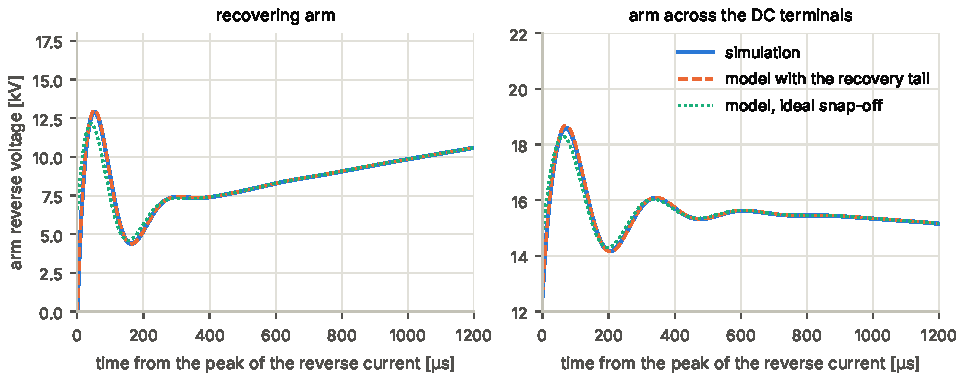
\includegraphics[width=\textwidth]{figures/fig_commutation_modes.pdf}
\caption{Voltage of the arm that turns off and of an arm across the DC terminals after the peak of the reverse current: simulation with $\Ld = \SI{\dsLdStiffSim}{\henry}$ and two-mode model with and without the tail of the reverse current.}
\label{fig:modes}
\end{figure}

\emph{DC side.} Table~\ref{tab:ld} shows the transition between the two limit cases of Sec.~\ref{sec:dcside}, with the load resistance unchanged. Up to $\Ld \approx \dsLdFlatRatio \times 2\Lc$ the arm stays at the crest; at $\Ld = 2\Lc = \SI{\dsLdStiff}{\milli\henry}$ the overshoot has started, and from about \dsLdNearStiffRatio{} times that value the arm voltage is within \SI{2}{\percent} of the stiff limit. The left panel of Fig.~\ref{fig:sharing} shows the same against the recovered charge: the model \eqref{eq:ktr} follows the simulation with $\Ld = \SI{\dsLdStiffSim}{\henry}$ from \dsQswLo{} to \SI{\dsQswHi}{\micro\coulomb}, a little on the high side because it uses the long-ramp value of $\Irr$.

\begin{table}[htb]
\centering\small
\caption{Effect of the DC inductance, simulation with the load resistance of the example ($u = \dsUunb$, nominal network).}
\label{tab:ld}
\begin{tabular}{@{}cccccccc@{}}
\toprule
$\Ld$ & $\Ld/(2\Lc)$ & $\Vs$ & $\ktr$ & $\Vw$ & \multicolumn{2}{c}{$P_{\Rsn}$ [W]} & resistors per \\
{[mH]} & & [kV] & & [kV] & weak & nominal & stack [W] \\
\midrule
\dsLdRows
\bottomrule
\end{tabular}
\end{table}

\emph{Hand values against the simulation.} Table~\ref{tab:hand} collects the hand calculation of this section and of Sec.~\ref{sec:dynamic}. The voltages are up to \SI{\dsHandVdevHi}{\percent} on the high side, the powers \dsHandPdevLo{} to \SI{\dsHandPdevHi}{\percent}. Most of the difference of the powers comes from the long-ramp value of $\Irr$, which the nominal diodes of the simulated unbalanced stack do not reach (\SI{\dsRIrrmN}{\ampere} in case \caseR{} and \SI{\dsLIrrmN}{\ampere} in case \caseL{} against \SI{\dsIrrHand}{\ampere}) and which enters with its square. The rest is the bound $f\Rsn\Irr\Delta Q$ on the extra loss of the weak level, \SI{\dsPwExtra}{\watt} against \SI{\dsPwExtraSimR}{\watt} and \SI{\dsPwExtraSimL}{\watt} in the simulation. The split of \eqref{eq:prsn} is \SI{\dsEstepLevel}{\milli\joule} for the steps and \SI{\dsEindLevel}{\milli\joule} for the inductance per level and period. Over the sweep of Fig.~\ref{fig:network}, \eqref{eq:prsn} evaluated with the simulated $\Irr$ stays within \SI{\dsPrsnDevLo}{\percent} and $+\SI{\dsPrsnDevHi}{\percent}$ of the simulated power of a nominal level in the two cases, for capacitors from \SI{\dsPrsnCLo}{\nano\farad} and resistors up to \SI{\dsPrsnRHi}{\ohm}. With larger resistors it is increasingly high, up to \SI{\dsPrsnDevTop}{\percent} at \SI{\dsNetRMax}{\ohm}, for the reason given in Sec.~\ref{sec:prsn}: in case \caseR{} with \SI{\dsCsn}{\nano\farad}, going from \dsNetRMin{} to \SI{\dsNetRMax}{\ohm} lowers the power of the snubber resistor of a nominal level from \SI{\dsNetRPnLo}{\watt} to \SI{\dsNetRPnHi}{\watt} and raises the turn-off loss of its diode from \SI{\dsNetRPrecLo}{\watt} to \SI{\dsNetRPrecHi}{\watt}.

\begin{table}[htb]
\centering\small
\caption{Hand calculation against the simulation, grid at $+\dsKgrid\,\%$, design recovery set, $u = \dsUunb$. The hand values of case \caseL{} are those of the stiff limit; the simulation with $\Ld = \SI{\dsLdStiffSim}{\henry}$ gives $\Vs = \SI{\dsStiffVs}{\kilo\volt}$ and $\Vw = \SI{\dsStiffVw}{\kilo\volt}$.}
\label{tab:hand}
\begin{tabular}{@{}lcccc@{}}
\toprule
 & \multicolumn{2}{c}{\caseR{} resistive load} & \multicolumn{2}{c}{\caseL{} smoothing reactor, \SI{\dsLdL}{\henry}} \\
\cmidrule(lr){2-3}\cmidrule(l){4-5}
 & hand & simulation & hand & simulation \\
\midrule
highest arm voltage $\Vs$ [kV] & \dsHandRVs & \dsRVs & \dsHandLVs & \dsLVs \\
weak level $\Vw$ [kV] & \dsHandRVw & \dsRVpkW & \dsHandLVw & \dsLVpkW \\
weak level, $\Csn$ \SI{\pm\dsTolC}{\percent} [kV] & \dsHandRVwTol & \dsRCtolVpkW & \dsHandLVwTol & \dsLCtolVpkW \\
$P_{\Rsn}$ of a nominal level [W] & \dsHandRPn & \dsRPrsnN & \dsHandLPn & \dsLPrsnN \\
$P_{\Rsn}$ of the weak level [W] & \dsHandRPw & \dsRPrsnW & \dsHandLPw & \dsLPrsnW \\
\bottomrule
\end{tabular}
\end{table}

\emph{Network.} Figure~\ref{fig:network} and Table~\ref{tab:net} show the simulated sweep of $\Csn$ and $\Rsn$. With the resistive load the peak of the weak level is set by the capacitor, as \eqref{eq:vw} says: with \SI{\dsRsn}{\ohm} it falls from \SI{\dsNetRVwCLo}{\kilo\volt} at \SI{\dsNetCMin}{\nano\farad} to \SI{\dsNetRVwCHi}{\kilo\volt} at \SI{\dsNetCMax}{\nano\farad}, and from \SI{\dsCsn}{\nano\farad} upwards it does not depend on the resistor between \dsNetRMin{} and \SI{\dsNetRNext}{\ohm}. The two limits of the resistor of Sec.~\ref{sec:rsnchoice} appear at the edges of the sweep. With \SI{\dsNetRMax}{\ohm} the peak moves from the crest to the turn-off of the arm: \eqref{eq:rstep} gives a snubber current of \SI{\dsIsnWeakHand}{\ampere} and a step of \SI{\dsNetRTopStepHand}{\kilo\volt}, above the \SI{\dsRVpkW}{\kilo\volt} that the level reaches at the crest; the simulation gives \SI{\dsNetRTopIsn}{\ampere}, \SI{\dsNetRTopStep}{\kilo\volt} on the resistor and a peak of \SI{\dsNetRTopVw}{\kilo\volt}, \SI{\dsNetRTopRel}{\percent} above the value at the crest. In the opposite corner, \SI{\dsNetCMin}{\nano\farad} with \SI{\dsNetRMin}{\ohm} ($\zeta_1 = \dsCornerZetaOne$, $\chi_1 = \dsCornerChiOne$), the oscillation that follows the turn-off brings the nominal levels back to zero, their diodes conduct again for a short time and the offset changes: along the row of \SI{\dsNetCMin}{\nano\farad} the peak of the weak level moves by up to \SI{\dsNetRSpreadHi}{\percent}.

With the smoothing reactor the peak depends on the resistor as well, with the flat minimum of \eqref{eq:rsn}: the relation gives \SI{\dsRsnHalfZeta}{\ohm} for \SI{\dsCsn}{\nano\farad}, and the model places the minimum of the arm voltage at \SI{\dsRsnOptTwo}{\ohm}, within \SI{1}{\percent} from \dsRsnOptLo{} to \SI{\dsRsnOptHi}{\ohm}. In the simulation the lowest peak of the weak level is at \SI{\dsNetLBestR}{\ohm}: against \SI{\dsRsn}{\ohm} it is \SI{\dsNetLBestRel}{\percent} lower, with \SI{\dsNetLBestPRel}{\percent} more power in the resistor of the weak level. At \SI{\dsNetRMax}{\ohm} the resistive step takes over here too. The power of the resistor of the weak level grows with the capacitor and with the resistor in both cases.

\begin{table}[htb]
\centering\small
\caption{Sweep of the network: peak of the weak level [kV] and power of its snubber resistor [W], by $\Csn$ (rows) and $\Rsn$ (columns, in ohm).}
\label{tab:net}
\begin{tabular}{@{}c|cccc|cccc||cccc|cccc@{}}
\toprule
 & \multicolumn{8}{c||}{peak of the weak level [kV]} & \multicolumn{8}{c}{$P_{\Rsn}$ of the weak level [W]} \\
$\Csn$ & \multicolumn{4}{c|}{\caseR{}} & \multicolumn{4}{c||}{\caseL{}} & \multicolumn{4}{c|}{\caseR{}} & \multicolumn{4}{c}{\caseL{}} \\
{[nF]} & \dsNetHead{} & \dsNetHead{} & \dsNetHead{} & \dsNetHead{} \\
\midrule
\dsNetRows
\bottomrule
\end{tabular}
\end{table}

\emph{Options for the current-stiff case.} With the smoothing reactor the nominal network leaves the weak level at \SI{\dsLCtolVpkW}{\kilo\volt} with the capacitor tolerance, \SI{\dsLCtolUtilW}{\percent} of $\Vrrm$. Table~\ref{tab:opt} compares the ways out. A larger capacitor with a resistor near \eqref{eq:rsn} brings the level back to $\ku\Vrrm$ (\SI{\dsOptAC}{\nano\farad} with \SI{\dsOptAR}{\ohm}, \SI{\dsOptAPresRel}{\percent} more losses in the resistors) or below it (\SI{\dsOptBC}{\nano\farad} with \SI{\dsOptBR}{\ohm}, \SI{\dsOptBPresRel}{\percent} more). One more level does the same with \SI{\dsOptPlusPresRel}{\percent} lower losses in the resistors, and the two together give a margin. A damper across the DC terminals removes about half of the overshoot ($\ktr$ of \dsDampKtrLo{} to \dsDampKtrHi{} instead of \dsKtrL{}), but it dissipates \dsDampPLo{} to \SI{\dsDampPHi}{\watt} and is itself a high-voltage component.

\begin{table}[!htb]
\centering\small
\caption{Case \caseL{}: options, simulated with the capacitor tolerance of \SI{\pm\dsTolC}{\percent} where not stated otherwise.}
\label{tab:opt}
\begin{tabular}{@{}lccccccc@{}}
\toprule
 & $\Vw$ & of $\Vrrm$ & $\Vs$ & \multicolumn{2}{c}{$P_{\Rsn}$ [W]} & resistors per & DC damper \\
Option & [kV] & [\%] & [kV] & weak & nominal & stack [W] & [W] \\
\midrule
\dsOptRows
\bottomrule
\end{tabular}
\end{table}

\emph{Ratings.} The \SI{70}{\percent} rule, applied to the peak of the weak level with the tolerances of $\Csn$ and $\Rb$, gives a rated capacitor voltage of at least \SI{\dsCapUnR}{\kilo\volt} in case \caseR{} and \SI{\dsCapUnL}{\kilo\volt} in case \caseL{}. The capacitor of the weak level carries \SI{\dsRIsnrmsW}{\ampere} rms and \SI{\dsRIsnpkW}{\ampere} peak (\SI{\dsLIsnrmsW}{\ampere} and \SI{\dsLIsnpkW}{\ampere} in case \caseL{}), a slope of \SI{\dsDvdtR}{\volt\per\micro\second} (\SI{\dsDvdtL}{\volt\per\micro\second}). Its resistor takes \SI{\dsEsnR}{\joule} per period (\SI{\dsEsnL}{\joule}) and a peak of \SI{\dsVrsnPkR}{\kilo\volt} (\SI{\dsVrsnPkL}{\kilo\volt}); an impulse of \SI{\dsUimpLevel}{\kilo\volt} across the level drives \SI{\dsIimp}{\ampere} through it. With $C_\mathrm{j}$ between \dsCjLo{} and \SI{\dsCjHi}{\nano\farad} (estimate), \eqref{eq:ls} limits the loop inductance to \SIrange{\dsLsLimLo}{\dsLsLimHi}{\micro\henry}. The thermal check of the resistors is in Sec.~\ref{sec:ex-thermal}.

\begin{figure}[!htb]
\centering
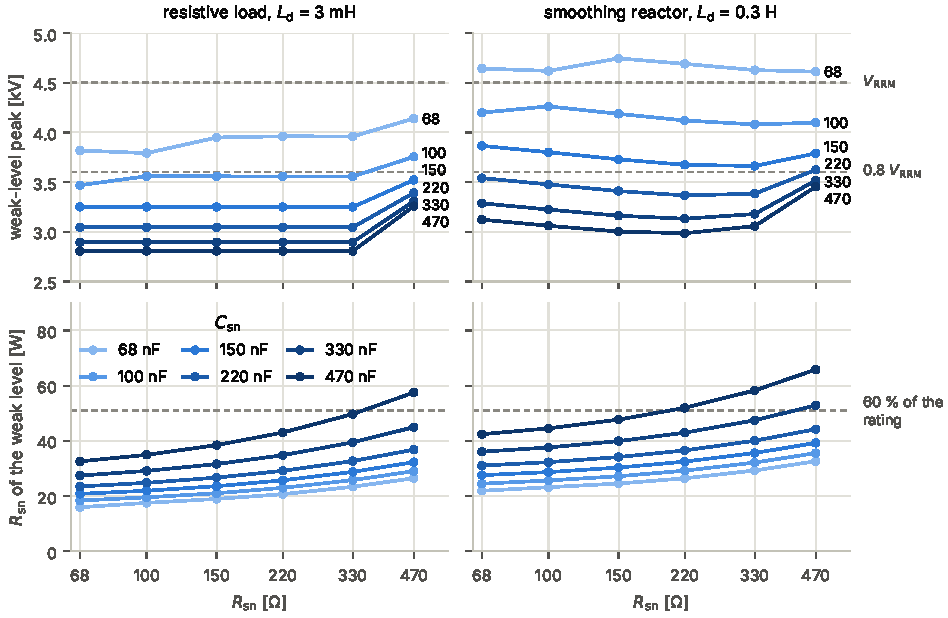
\includegraphics[width=\textwidth]{figures/fig_network_sweep.pdf}
\caption{Simulated peak of the weak level and power of its snubber resistor against $\Rsn$, for \dsNetCCount{} values of $\Csn$ (design recovery set, $u = \dsUunb$, no tolerances).}
\label{fig:network}
\end{figure}

%=====================================================================
\section{Losses and thermal design}
\label{sec:thermal}
\subsection{Losses of a diode}
A diode of the stack has three loss terms.
\begin{itemize}
\item \emph{Forward loss.} With the threshold voltage $V_\mathrm{T0}$ and the slope resistance $r_\mathrm{T}$ of the datasheet,
\begin{equation}
P_\mathrm{F} = V_\mathrm{T0}\,I_\mathrm{F(AV)} + r_\mathrm{T}\,I_\mathrm{F(rms)}^2, \qquad I_\mathrm{F(AV)} = \frac{\Id}{3}, \quad I_\mathrm{F(rms)} \simeq \frac{\Id}{\sqrt3} .
\label{eq:pf}
\end{equation}
\item \emph{Turn-off loss.} During the tail the diode carries the decaying reverse current while its voltage rises. At line frequency this is a few watts, and the simulation gives it directly.
\item \emph{Reverse loss.} A blocking diode dissipates the product of its voltage and its leakage current,
\begin{equation}
P_\mathrm{R}(\Tj) = \frac1T \int_0^T v(t)\,\Ilk\big(v(t), \Tj\big)\,dt ,
\label{eq:pr}
\end{equation}
with the leakage current of \eqref{eq:ilk}. It is largest on the weak level, which blocks the highest voltage, and it grows steeply with the temperature: with the curves of App.~\ref{app:data} the leakage doubles about every \SI{12}{\kelvin} above \SI{100}{\celsius}.
\end{itemize}
The devices of a stack are chosen for their voltage and are often far larger than the load current asks for. The forward loss is then small, and the reverse loss of a diode at the leakage limit is not negligible against it.

\subsection{Thermal stability of the blocking diode}
The junction temperature is the solution of
\begin{equation}
\Tj = T_\mathrm{a} + R_\mathrm{th(j\text{-}a)}\left[P_\mathrm{F} + P_\mathrm{off} + P_\mathrm{R}(\Tj)\right], \qquad R_\mathrm{th(j\text{-}a)} = R_\mathrm{th(j\text{-}c)} + R_\mathrm{th(c\text{-}h)} + \Rthha ,
\label{eq:tj}
\end{equation}
where $P_\mathrm{off}$ is the turn-off loss and $\Rthha$ the thermal resistance from the heat sink of one diode to the cooling air at $T_\mathrm{a}$. Because $P_\mathrm{R}$ grows with $\Tj$, the equilibrium is stable only as long as the heat sink removes heat faster than the leakage generates it,
\begin{equation}
\frac{dP_\mathrm{R}}{d\Tj} < \frac{1}{R_\mathrm{th(j\text{-}a)}} ,
\label{eq:runaway}
\end{equation}
and above a critical thermal resistance \eqref{eq:tj} has no solution: the diode runs away. The heat sink therefore has two limits, the resistance that keeps the design temperature and the resistance at which a diode at the leakage limit on the weak level runs away. The ratio of the two is the thermal margin of the stack, and it is the number to look at when the cooling air is hot.

The design junction temperature is a choice. A value well below the maximum of the datasheet pays three times: the leakage current falls by a decade, and with it the static unbalance and the reverse loss; the recovered charge falls with the lifetime (Sec.~\ref{sec:recovery}); and the distance from the runaway grows.

\subsection{Resistors}
Each level has two resistors that dissipate continuously: $\Rb$ with $V_\mathrm{rms}^2/\Rb$ and $\Rsn$ with \eqref{eq:prsn}. Any level can be the weak one, so every resistor is rated for the weak level, while the heat to remove is that of one weak and $n-1$ nominal levels per arm. The temperature of the element follows from its derating curve. With a rated power $P_\mathrm{n}$ in air at $T_\mathrm{n}$ and a linear derating to zero at $T_\mathrm{max}$, an element that dissipates $P$ in air at $T_\mathrm{a}$ reaches about
\begin{equation}
T \simeq T_\mathrm{a} + \left(T_\mathrm{max} - T_\mathrm{n}\right)\frac{P}{P_\mathrm{n}} ,
\label{eq:tres}
\end{equation}
and its rating at the air temperature of the stack is $P_\mathrm{n}(T_\mathrm{max} - T_\mathrm{a})/(T_\mathrm{max} - T_\mathrm{n})$. The \SI{60}{\percent} rule of Sec.~\ref{sec:ratings} applies to this derated value. The linear derating is an assumption when the datasheet gives the rated point only.

\subsection{Losses of the stack and air flow}
A stack dissipates $n$ diode losses plus the losses of its resistors, and a bridge has six stacks. The air flow that removes the power $P$ with a temperature rise $\Delta T$ is
\begin{equation}
\dot V = \frac{P}{\rho\,c_p\,\Delta T}, \qquad \rho \simeq \SI{1.204}{\kilo\gram\per\cubic\metre}\;\frac{293}{273 + T_\mathrm{a}}\;e^{-h/\SI{8434}{\metre}} ,
\label{eq:flow}
\end{equation}
with $c_p = \SI{1007}{\joule\per\kilo\gram\per\kelvin}$, the inlet temperature $T_\mathrm{a}$ in \si{\celsius} and the altitude $h$. The order of the components in the air stream matters as much as the flow: the film capacitors have the lowest temperature limit and come first, then the heat sinks of the diodes, then the resistors, whose surfaces are the hottest parts of the stack. With natural convection the same order holds from bottom to top. The air that has passed the resistors should not reach capacitors or diodes of another stack.

\subsection{Worked example}
\label{sec:ex-thermal}
\emph{Diodes.} At the grid at $+\dsKgrid\,\%$ an arm carries $I_\mathrm{F(AV)} = \SI{\dsRIfav}{\ampere}$ and $I_\mathrm{F(rms)} = \SI{\dsRIfrms}{\ampere}$, and \eqref{eq:pf} gives $P_\mathrm{F} = \SI{\dsPfR}{\watt}$ with $V_\mathrm{T0} = \SI{\dsVto}{\volt}$ and $r_\mathrm{T} = \SI{\dsRt}{\milli\ohm}$. The simulated turn-off loss is \SI{\dsRPrecN}{\watt} in case \caseR{} and \SI{\dsLPrecN}{\watt} in case \caseL{}. The reverse loss \eqref{eq:pr} of a diode at the leakage limit on the weak level is \SI{\dsPrWRNinety}{\watt} at \SI{90}{\celsius}, \SI{\dsPrWRHundred}{\watt} at \SI{100}{\celsius} and \SI{\dsPrWRHundredTwentyFive}{\watt} at \SI{125}{\celsius} (\SI{\dsPrNRHundred}{\watt} at \SI{100}{\celsius} on a nominal level).

With $R_\mathrm{th(j\text{-}c)} + R_\mathrm{th(c\text{-}h)} = \SI{\dsRthJh}{\kelvin\per\watt}$ and air at \SI{\dsTa}{\celsius}, Table~\ref{tab:tj} gives the junction temperature against the heat sink. The design temperature of \SI{\dsTjDes}{\celsius} on the weak level asks for $\Rthha \le \SI{\dsRhaRDes}{\kelvin\per\watt}$ in case \caseR{} and \SI{\dsRhaLDes}{\kelvin\per\watt} in case \caseL{}, where the diode dissipates \SI{\dsPdR}{\watt} and \SI{\dsPdL}{\watt}. The weak level runs away above \SI{\dsRhaRRun}{\kelvin\per\watt} and \SI{\dsRhaLRun}{\kelvin\per\watt} (Fig.~\ref{fig:thermal}): the margin on the thermal resistance is a factor of \dsRhaRRatio{}. Without the reverse loss the same diode could reach its maximum junction temperature with \SI{\dsRhaRCond}{\kelvin\per\watt}: what sizes the heat sink is the hot air and the leakage limit.

\begin{table}[htb]
\centering\small
\caption{Junction temperature [\si{\celsius}] against the thermal resistance from the heat sink to air at \SI{\dsTa}{\celsius}: without reverse loss, and with a diode at the leakage limit on a nominal level and on the weak level.}
\label{tab:tj}
\begin{tabular}{@{}c|ccc|ccc@{}}
\toprule
 & \multicolumn{3}{c|}{\caseR{} resistive load} & \multicolumn{3}{c}{\caseL{} smoothing reactor} \\
$\Rthha$ [K/W] & no leakage & nominal & weak & no leakage & nominal & weak \\
\midrule
\dsTjRows
\bottomrule
\end{tabular}
\end{table}

\begin{figure}[htb]
\centering
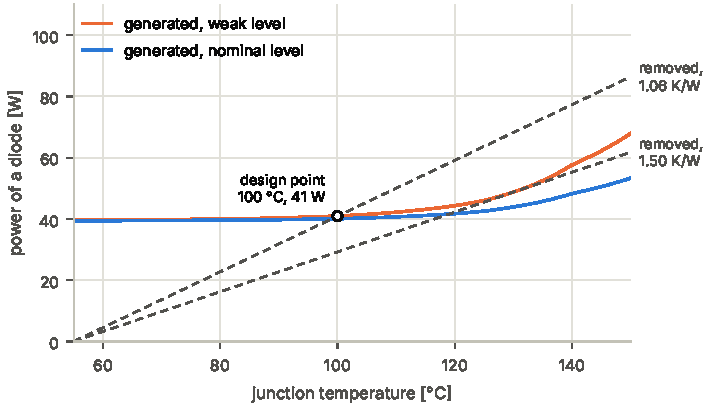
\includegraphics[width=0.72\textwidth]{figures/fig_thermal_stability.pdf}
\caption{Thermal stability of a diode at the leakage limit, case \caseL{}: generated power against the junction temperature and power removed by the heat sink for the two limits of $\Rthha$. The line of the higher resistance is tangent to the curve of the weak level.}
\label{fig:thermal}
\end{figure}

\emph{Resistors.} The element assumed for $\Rb$ and $\Rsn$ is rated \SI{\dsRpn}{\watt} in air at \SI{\dsRtn}{\celsius}, with a linear derating to zero at \SI{\dsRtmax}{\celsius} (App.~\ref{app:data}). In air at \SI{\dsTa}{\celsius} its rating falls to \SI{\dsPmax}{\watt}, of which \SI{\dsKp}{\percent} are \SI{\dsPrsnSixty}{\watt}, with the element at \SI{\dsTresLim}{\celsius} by \eqref{eq:tres}. Table~\ref{tab:res} lists the simulated powers and the temperatures from \eqref{eq:tres}. The snubber resistor of the weak level uses \SI{\dsPrsnUseR}{\percent} of the derated rating in case \caseR{} and \SI{\dsPrsnUseL}{\percent} in case \caseL{}: it is inside the \SI{\dsKp}{\percent} rule, with margin for a larger recovered charge (Table~\ref{tab:qsweep}) and for the state with one level failed (\SI{\dsPrsnUseShort}{\percent}). The balancing resistors have a larger margin. A smaller element would be enough for the power; the choice also has to consider the peak and impulse voltages on the element (Sec.~\ref{sec:ex-transient}).

\begin{table}[htb]
\centering\small
\caption{Resistors of a level: simulated power and temperature of the element from \eqref{eq:tres}, air at \SI{\dsTa}{\celsius}, nominal network.}
\label{tab:res}
\begin{tabular}{@{}lcccc@{}}
\toprule
 & \multicolumn{2}{c}{\caseR{} resistive load} & \multicolumn{2}{c}{\caseL{} smoothing reactor} \\
\cmidrule(lr){2-3}\cmidrule(l){4-5}
 & weak level & nominal level & weak level & nominal level \\
\midrule
$\Rsn$: power [W] & \dsRPrsnW & \dsRPrsnN & \dsLPrsnW & \dsLPrsnN \\
$\Rsn$: temperature [\si{\celsius}] & \dsThsRsnRW & \dsThsRsnRN & \dsThsRsnLW & \dsThsRsnLN \\
$\Rb$: power [W] & \dsRPrbW & \dsRPrbN & \dsLPrbW & \dsLPrbN \\
$\Rb$: temperature [\si{\celsius}] & \dsThsRbRW & \dsThsRbRN & \dsThsRbLW & \dsThsRbLN \\
\bottomrule
\end{tabular}
\end{table}

\emph{Stack and air flow.} The resistors of a stack dissipate \SI{\dsRPres}{\watt} in case \caseR{} and \SI{\dsLPres}{\watt} in case \caseL{}, its \dsNword{} diodes \SI{\dsPdiodesR}{\watt} and \SI{\dsPdiodesL}{\watt} with every diode at the leakage limit: the resistors are \SI{\dsPresShareR}{\percent} and \SI{\dsPresShareL}{\percent} of the losses of the stack. A stack dissipates \SI{\dsPstackR}{\watt} and \SI{\dsPstackL}{\watt}, the bridge \SI{\dsPbridgeR}{\kilo\watt} and \SI{\dsPbridgeL}{\kilo\watt}. With air at \SI{\dsTa}{\celsius} and \SI{\dsAltitude}{\metre} the density is \SI{\dsRho}{\kilo\gram\per\cubic\metre}, and \eqref{eq:flow} asks for \SI{\dsFlowR}{\cubic\metre\per\hour} and \SI{\dsFlowL}{\cubic\metre\per\hour} for a rise of \SI{10}{\kelvin} over the bridge.

%=====================================================================
\section{Insulation}
\label{sec:insulation}
\subsection{Voltages inside the stack}
The heat sinks of a stack are live, each at the potential of a node of the string, and the resistors and the capacitor of a level bridge two adjacent heat sinks. Between two parts of the stack that are $m$ levels apart three voltages are needed.
\begin{itemize}
\item The \emph{rms working voltage} sets the creepage distance. It is taken at the rated grid voltage, with the weak level among the $m$.
\item The \emph{repetitive peak} sets the requirements on solid insulation and on partial discharge. It is taken at the highest grid voltage and includes the commutation transient. With the charge model of Sec.~\ref{sec:dynamic}, $m$ adjacent levels that include the weak one reach $\tfrac{m}{n}\Vs + \tfrac{n-m}{n}\Delta v$.
\item The \emph{impulse withstand voltage} sets the clearance. A surge across the stack divides on the snubber capacitors, and each diode limits the voltage of its own level when it reaches its breakdown voltage. Air and surfaces across a level should withstand more than the device does. Here the impulse voltage of a level, $U_\mathrm{imp}$, is chosen as the standard value next above $1.3\,\Vrsm$, and $m$ levels are assigned $m\,U_\mathrm{imp}$.
\end{itemize}

\subsection{Distances}
For the distances inside the stack the tables of IEC~60664-1 are the usual reference \cite{iec60664}: Table~F.2 gives the clearance against the impulse withstand voltage (case~A, inhomogeneous field, up to \SI{2000}{\metre}) and Table~F.5 of the 2020 edition (Table~F.4 of the 2007 edition) the creepage distance against the rms voltage, by pollution degree and material group. Three remarks apply.
\begin{itemize}
\item The scope of the standard ends at \SI{1000}{\volt} AC and \SI{1500}{\volt} DC, although its tables go further. For converters above these voltages the product standard has to be consulted \cite{iec62477}; the tables are used here for the first sizing.
\item Recurring peaks are a separate requirement. The standard has a table of clearances for steady-state and recurring peak voltages (F.8 in the 2020 edition) and one for the avoidance of partial discharge (F.9), and with several kilovolts of repetitive peak per level they have to be checked next to the impulse value. Solid insulation between levels (pads, resistor bodies, capacitor cases, clamping rods) has to be free of partial discharge at the repetitive peak.
\item Above \SI{2000}{\metre} the clearances are multiplied by the altitude factor of the standard.
\end{itemize}

\subsection{Insulation to earth}
The voltage of the stack to earth depends on the earthing of the system and not on the stack. Four cases cover most installations: (A) the neutral of the AC side is earthed; (B) one DC pole is earthed; (C) the midpoint of the DC side is earthed; (D) one AC phase is earthed, which is also the first earth fault of an unearthed system. In cases A and C the DC poles sit at about half the DC voltage to earth. In case B the other pole and the AC terminals carry the full voltage. An unearthed system has to be designed for its first fault, that is for the worse of B and D.

The withstand voltages to earth are not derived from the working voltage. They come from the insulation coordination of the installation: the highest voltage for equipment $U_\mathrm{m}$ of the AC side selects a standard pair of power-frequency and lightning-impulse withstand voltages \cite{iec60071}, the surge arresters are chosen to match, and the clearances to earth and between phases follow from the lightning-impulse level. The creepage distance to earth is taken from the rms voltage to earth of the worst earthing case.

\subsection{Worked example}
The impulse voltage of a level is $U_\mathrm{imp} = \SI{\dsUimpLevel}{\kilo\volt}$, \dsUimpRatio{} times $\Vrsm$. Table~\ref{tab:ins} lists the voltages across $m$ levels and the distances from the tables, Table~\ref{tab:earth} the voltages to earth of the most stressed node of the stack. The distances are table values without altitude correction and without margin; the tables are transcribed in App.~\ref{app:data}.

\begin{table}[htb]
\centering\small
\caption{Voltages across $m$ adjacent levels that include the weak one (rms at the rated grid voltage, simulated peak at $+\dsKgrid\,\%$) and distances from IEC~60664-1: clearance for $m\,U_\mathrm{imp}$, creepage for pollution degree~2.}
\label{tab:ins}
\begin{tabular}{@{}cccccccc@{}}
\toprule
 & rms & \multicolumn{2}{c}{repetitive peak [kV]} & impulse & clearance & \multicolumn{2}{c}{creepage [mm]} \\
\cmidrule(lr){3-4}\cmidrule(l){7-8}
$m$ & [kV] & \caseR{} & \caseL{} & [kV] & [mm] & group I & group III \\
\midrule
\dsInsRows
\bottomrule
\end{tabular}
\end{table}

\begin{table}[htb]
\centering\small
\caption{Highest voltage of a node of the stack to earth for four ways of earthing the system (rms at the rated grid voltage, simulated peak at $+\dsKgrid\,\%$) and creepage distance from IEC~60664-1, pollution degree~2.}
\label{tab:earth}
\begin{tabular}{@{}clccccc@{}}
\toprule
 & & rms & \multicolumn{2}{c}{peak [kV]} & \multicolumn{2}{c}{creepage [mm]} \\
\cmidrule(lr){4-5}\cmidrule(l){6-7}
Case & Earthing & [kV] & \caseR{} & \caseL{} & group I & group III \\
\midrule
\dsEarthRows
\bottomrule
\end{tabular}
\end{table}

Across one level the clearance is \SI{\dsClearOne}{\milli\metre} and the creepage \dsCreepIOne{} to \SI{\dsCreepIIIOne}{\milli\metre}, according to the material; across the stack they are \SI{\dsClearAll}{\milli\metre} and \dsCreepIAll{} to \SI{\dsCreepIIIAll}{\milli\metre}. The commutation transient of case \caseL{} raises the repetitive peaks by \dsInsRiseLo{} to \SI{\dsInsRiseHi}{\percent} and leaves the rms values unchanged. To earth, one earthed DC pole doubles the rms voltage of the earthed neutral (factor \dsEarthRatioBA{}), and with it the creepage distance. For the AC side of the example, $U_\mathrm{m} = \SI{12}{\kilo\volt}$, the standard lightning-impulse withstand voltages are 60, 75 and \SI{95}{\kilo\volt} with a power-frequency withstand voltage of \SI{28}{\kilo\volt}, and the corresponding clearances in air are 90, 120 and \SI{160}{\milli\metre}; these values are quoted from memory and have to be checked on the standard.

%=====================================================================
\section{Faults and abnormal conditions}
\label{sec:faults}
\subsection{Short circuit on the DC side}
A short circuit at the DC terminals is limited by the commutation inductance only. The steady-state current on the AC side and its first peak are
\begin{equation}
I_\mathrm{k} = \frac{I_\mathrm{TN}}{\uk}, \qquad \hat\imath_\mathrm{k} = \kappa\,\sqrt2\,I_\mathrm{k},
\label{eq:ik}
\end{equation}
with $I_\mathrm{TN}$ the rated current of the transformer and $\kappa$ up to 1.8. Each arm carries half waves of this current until the protection clears the fault, with $I^2t = (\sqrt2\,I_\mathrm{k})^2/(4f)$ per half wave. The checks are the peak against $I_\mathrm{FSM}$ and the $I^2t$ against the rating of the device, at the lowest $\uk$ and for the clearing time of the protection; for more than one half wave the surge-current curve of the datasheet applies. Devices chosen for their voltage are usually so large that this check is not the limiting one. After the surge the junction is hot, however, and the reverse voltage that returns is shared worse than in normal operation, because leakage and recovered charge grow with the temperature: the surge rating to use is the one with reapplied voltage.

\subsection{One device failed short}
Press-pack devices fail to a short circuit, and the arm goes on with $n - 1$ levels. To a first approximation the level voltages grow by $n/(n-1)$ and the losses of the resistors by the square of it; \eqref{eq:vwtol} with $n - 1$ gives the peak of the weak level. Two decisions belong to the specification of the stack. The first is whether the bridge has to stay in service in this state: if so, the criteria of Sec.~\ref{sec:number} are applied to $n - 1$ levels, possibly with a higher $\ku$ for a limited time. The second is how the failure is detected. Without a monitor of the level voltages the failure stays hidden, and the next one is likely to take the whole arm.

\subsection{Lowest short-circuit voltage, light load, no load}
A lower $\uk$ raises the slope $\alpha$ and with it $\Qrr$ and $\Irr$, while the overlap and $\Vo$ become smaller: the charge difference and the offset of the weak level grow, the losses of the snubber change little. At light load the ramp is shorter and the charge smaller, so the design case remains full load. With the DC side open the arms block a voltage with a DC component, which is shared by the balancing resistors (Sec.~\ref{sec:rbrole}); after de-energisation the same resistors discharge the snubber capacitors with $\taus$.

\subsection{Surges and switching}
Surges from the grid and the switching of the transformer reach the bridge through the transformer. Surge arresters at the AC terminals limit them, and their protection level is coordinated with the non-repetitive rating of the levels: in a fast surge the share of a level is fixed by the snubber capacitors, $(1+c)/(n - (n-2)c)$ of the arm voltage for the level with the smallest capacitor, on top of the offset that the level already carries. On the DC side a diode bridge is its own free-wheeling path: when the AC side is opened under load, the current of a DC reactor decays through the legs of the bridge and produces no overvoltage on the stacks.

\subsection{Worked example}
With $I_\mathrm{TN} = \SI{\dsItn}{\ampere}$, \eqref{eq:ik} gives a short-circuit current of \SI{\dsIk}{\ampere} rms with a first peak of \SI{\dsIkPk}{\kilo\ampere}; at $\uk = \dsUkMin\,\%$ they are \SI{\dsIkMin}{\ampere} and \SI{\dsIkPkMin}{\kilo\ampere}, with $I^2t = \SI{\dsItwoHwMin e3}{\ampere\squared\second}$ per half wave. The assumed diode is rated $I_\mathrm{FSM} = \SI{\dsIfsm}{\kilo\ampere}$ and $I^2t = \SI{\dsItwot e3}{\ampere\squared\second}$ for a half sine of \SI{10}{\milli\second} with reapplied reverse voltage: the peak is \SI{\dsIkPkShare}{\percent} of the rating and the surge is not a constraint.

With one level shorted the weak level reaches \SI{\dsRShortVpkW}{\kilo\volt} in case \caseR{}, \SI{\dsRShortUtilW}{\percent} of $\Vrrm$, and \SI{\dsLShortVpkW}{\kilo\volt} in case \caseL{}, \SI{\dsLShortUtilW}{\percent}, both without the capacitor tolerance; its snubber resistor takes \SI{\dsRShortPrsnW}{\watt} and \SI{\dsLShortPrsnW}{\watt}. With the capacitor tolerance the peaks are \SI{\dsRShortCtolVpkW}{\kilo\volt} (\SI{\dsRShortCtolUtilW}{\percent}) and \SI{\dsLShortCtolVpkW}{\kilo\volt} (\SI{\dsLShortCtolUtilW}{\percent}). With \dsNminusWord{} levels left, the stack on the resistive load rides through the failure with the weak level above $\ku\Vrrm$ but below $\Vrrm$. With the smoothing reactor the weak level exceeds $\Vrrm$ in the worst case and comes to $\Vrsm = \SI{\dsVrsm}{\kilo\volt}$: the first failure is likely to cause the next one.

At $\uk = \dsUkMin\,\%$ the simulated peak reverse current of a nominal diode is \SI{\dsRUkminIrrmN}{\ampere} instead of \SI{\dsRIrrmN}{\ampere}, and the weak level reaches \SI{\dsRUkminVpkW}{\kilo\volt} in case \caseR{} and \SI{\dsLUkminVpkW}{\kilo\volt} in case \caseL{}; the power of its snubber resistor is \SI{\dsRUkminPrsnW}{\watt} in case \caseR{}, against \SI{\dsRPrsnW}{\watt} at $\uk = \dsUk\,\%$. At half load the peaks are \SI{\dsRHalfVpkW}{\kilo\volt} and \SI{\dsLHalfVpkW}{\kilo\volt}.

%=====================================================================
\section{Worked example: summary}
\label{sec:summary}
Table~\ref{tab:summary} collects the results of the example for the two DC sides, and Table~\ref{tab:nsweep} repeats the simulation for other numbers of devices.

\begin{table}[htb]
\centering\small
\caption{Worked example, $n = \dsN$, $\Rb = \SI{\dsRb}{\kilo\ohm}$, $\Rsn = \SI{\dsRsn}{\ohm}$, $\Csn = \SI{\dsCsn}{\nano\farad}$, grid at $+\dsKgrid\,\%$, design recovery set with $u = \dsUunb$: simulated values unless stated.}
\label{tab:summary}
\begin{tabular}{@{}lcc@{}}
\toprule
 & \caseR{} resistive load & \caseL{} smoothing reactor \\
\midrule
DC voltage and current & \SI{\dsRVdc}{\kilo\volt}, \SI{\dsRIdc}{\ampere} & \SI{\dsLVdc}{\kilo\volt}, \SI{\dsLIdc}{\ampere} \\
Recovery of a nominal diode, $\Irr$ and $\Qrr$ & \SI{\dsRIrrmN}{\ampere}, \SI{\dsRQrrN}{\micro\coulomb} & \SI{\dsLIrrmN}{\ampere}, \SI{\dsLQrrN}{\micro\coulomb} \\
Highest arm voltage $\Vs$ and transient factor $\ktr$ & \SI{\dsRVs}{\kilo\volt}, \dsKtrR & \SI{\dsLVs}{\kilo\volt}, \dsKtrL \\
Weak level, peak & \SI{\dsRVpkW}{\kilo\volt} (\SI{\dsRUtilW}{\percent} of $\Vrrm$) & \SI{\dsLVpkW}{\kilo\volt} (\SI{\dsLUtilW}{\percent}) \\
Weak level, peak with $\Csn$ \SI{\pm\dsTolC}{\percent} and $\Rb$ \SI{\pm\dsTolRb}{\percent} & \SI{\dsRTolVpkW}{\kilo\volt} (\SI{\dsRTolUtilW}{\percent}) & \SI{\dsLTolVpkW}{\kilo\volt} (\SI{\dsLTolUtilW}{\percent}) \\
Nominal level, peak & \SI{\dsRVpkN}{\kilo\volt} & \SI{\dsLVpkN}{\kilo\volt} \\
Level voltage, rms, weak and nominal & \SI{\dsRVrmsW}{\kilo\volt}, \SI{\dsRVrmsN}{\kilo\volt} & \SI{\dsLVrmsW}{\kilo\volt}, \SI{\dsLVrmsN}{\kilo\volt} \\
$\Rsn$, power, weak and nominal level & \SI{\dsRPrsnW}{\watt}, \SI{\dsRPrsnN}{\watt} & \SI{\dsLPrsnW}{\watt}, \SI{\dsLPrsnN}{\watt} \\
$\Rb$, power, weak and nominal level & \SI{\dsRPrbW}{\watt}, \SI{\dsRPrbN}{\watt} & \SI{\dsLPrbW}{\watt}, \SI{\dsLPrbN}{\watt} \\
Resistors of a stack & \SI{\dsRPres}{\watt} & \SI{\dsLPres}{\watt} \\
Diode at the leakage limit, \SI{\dsTjDes}{\celsius}, weak level & \SI{\dsPdR}{\watt} & \SI{\dsPdL}{\watt} \\
$\Rthha$ for \SI{\dsTjDes}{\celsius}; runaway above & \SI{\dsRhaRDes}{\kelvin\per\watt}; \SI{\dsRhaRRun}{\kelvin\per\watt} & \SI{\dsRhaLDes}{\kelvin\per\watt}; \SI{\dsRhaLRun}{\kelvin\per\watt} \\
Losses of a stack and of the bridge & \SI{\dsPstackR}{\watt}, \SI{\dsPbridgeR}{\kilo\watt} & \SI{\dsPstackL}{\watt}, \SI{\dsPbridgeL}{\kilo\watt} \\
Charge $\Qrr$ that brings the weak level to $\ku\Vrrm$; with $\Csn$ \SI{\pm\dsTolC}{\percent} & \SI{\dsQlimVR}{\micro\coulomb}; \SI{\dsQlimVTolR}{\micro\coulomb} & \SI{\dsQlimVL}{\micro\coulomb}; \SI{\dsQlimVTolL}{\micro\coulomb} \\
Unbalance that brings the weak level to $\ku\Vrrm$ (design charge) & \dsUlimDesR & \dsUlimDesL \\
One level failed short: weak level, peak & \SI{\dsRShortVpkW}{\kilo\volt} (\SI{\dsRShortUtilW}{\percent}) & \SI{\dsLShortVpkW}{\kilo\volt} (\SI{\dsLShortUtilW}{\percent}) \\
One level failed short, with $\Csn$ \SI{\pm\dsTolC}{\percent} & \SI{\dsRShortCtolVpkW}{\kilo\volt} (\SI{\dsRShortCtolUtilW}{\percent}) & \SI{\dsLShortCtolVpkW}{\kilo\volt} (\SI{\dsLShortCtolUtilW}{\percent}) \\
\bottomrule
\end{tabular}
\end{table}

\begin{table}[htb]
\centering\small
\caption{Number of devices in series: simulated peak of the weak level, without and with the capacitor tolerance of \SI{\pm\dsTolC}{\percent}, and losses of the resistors of a stack (network of the example).}
\label{tab:nsweep}
\begin{tabular}{@{}c|cccc|cccc@{}}
\toprule
 & \multicolumn{4}{c|}{\caseR{} resistive load} & \multicolumn{4}{c}{\caseL{} smoothing reactor} \\
 & $\Vw$ & with tol. & of $\Vrrm$ & resistors & $\Vw$ & with tol. & of $\Vrrm$ & resistors \\
$n$ & [kV] & [kV] & [\%] & [W] & [kV] & [kV] & [\%] & [W] \\
\midrule
\dsNRows
\bottomrule
\end{tabular}
\end{table}

The reading of the two tables is the following.
\begin{itemize}
\item With a resistive load \dsNword{} devices meet the criterion $\ku = \dsKu\,\%$ with the tolerances, and the network keeps it up to a charge of \SI{\dsQlimVTolR}{\micro\coulomb} with the capacitor tolerance, just above the upper scenario. The resistors work at less than half of their rating at the air temperature of the stack, and the heat sink has a factor of \dsRhaRRatio{} to the runaway limit.
\item With a current-stiff DC side the same stack works at \SI{\dsLTolUtilW}{\percent} of $\Vrrm$. The commutation transient costs one device: \dsNplusWord{} levels, or \dsNword{} with a larger snubber, restore the criterion (Table~\ref{tab:opt}).
\item \dsNminusWordCap{} devices are not enough in either case, and the first cut \eqref{eq:n} had already said so.
\item What separates these outcomes is not in the datasheet of the diode. Two data have to be obtained before the stack is frozen: the recovered charge and the peak reverse current at the slope of the bridge, with their band, from the manufacturer or from a bench test; and the impedance of the DC side at the frequency of mode~2, here \SI{\dsFzTwo}{\kilo\hertz}.
\end{itemize}

%=====================================================================
\section{Design rules in short}
\label{sec:rules}
\begin{enumerate}
\item \emph{Operating point.} Compute $\mu$, $\Vo$ and $\alpha$ at the highest grid voltage, at the lowest $\uk$ and at light load. Expect a ramp of about half a millisecond, much longer than the carrier lifetime, and a slope one to two decades below the datasheet conditions.
\item \emph{Number of devices.} Start from $n \ge \ktr\ksh\Vh_\mathrm{max}/(\ku\Vrrm)$ with $\ku = 0.8$, $\ktr = 1$ for a damped DC side and 1.15 to 1.25 for a current-stiff one, $\ksh = 1.25$ to 1.35 for devices matched in recovered charge. Decide whether the bridge has to run with one device failed.
\item \emph{Leakage.} Use the leakage at the working voltage and temperature, not $\Irm$. Size $\Rb$ with the static criterion \eqref{eq:an2} at the highest resistance that satisfies it. In the running bridge $\Rb\Csn$ is longer than the blocking interval and the sharing is capacitive; $\Rb$ decides when the arm blocks a DC voltage and after de-energisation.
\item \emph{Recovered charge.} Do not scale the datasheet point, neither linearly nor along the datasheet curve. Bound the charge with the floor and the ceiling of Sec.~\ref{sec:recovery}, design between them, and ask the manufacturer for $Q_\mathrm{S}$ and $\Irr$ at the slope of the circuit and for a band at that slope. A band given at datasheet conditions is two to three times as wide in the bridge.
\item \emph{Dynamic sharing.} The weak level sits above its share by $\tfrac{n-1}{n}\Delta Q/\Csn$ for the whole blocking interval. Put the capacitor tolerance into the share as well, \eqref{eq:vwtol}. State the charge difference that the design tolerates.
\item \emph{Commutation transient.} The highest arm voltage is not on the arm that turns off but on the arms across the DC terminals, at the steps near the crest. With $\Ld \gg 2\Lc$ it is $\Vh + \tfrac12\Vos(F_2 - 1)$, about \SI{20}{\percent} above the crest for a snubber of ordinary size; a resistive DC side removes the overshoot. Simulate with the real DC side.
\item \emph{Snubber resistor.} With a current-stiff DC side choose $\Rsn \approx \sqrt{5\Lc/(n\Csn)}$; with a damped one the peak hardly depends on $\Rsn$. The loss is $f\,[\tfrac78\Csn(\Vos/n)^2 + \Lc\Irr^2/n]$ plus the line-frequency term, mostly the energy of the reverse current in $\Lc$, and it depends little on $\Rsn$. Keep the resistive step of the weak level at its turn-off, \eqref{eq:rstep}, well below the peak of the level. Rate every resistor for the weak level and keep it below \SI{60}{\percent} of its rating at the air temperature of the stack.
\item \emph{Snubber capacitor.} Rated voltage at least $\Vw/0.7$ with the tolerances; free of partial discharge at the repetitive peak; low series inductance; the tolerance assumed in the sharing calculation.
\item \emph{Layout.} Keep the loop of diode, $\Rsn$ and $\Csn$ below $\Rsn^2 C_\mathrm{j}/4$, a few microhenries. Use resistors of low inductance.
\item \emph{Thermal design.} Check the runaway limit of the blocking diode at the leakage limit, not only the junction temperature. Choose a design temperature well below the maximum. Lead the air over the capacitors first, then the diodes, then the resistors.
\item \emph{Insulation.} Assign an impulse voltage to each level above the breakdown of the device and size the distances for $m$ levels. Take the insulation to earth from the insulation coordination of the installation and from its earthing.
\item \emph{Faults.} Check the surge current at the lowest $\uk$ with reapplied voltage, the state with $n - 1$ levels and the coordination of the arresters with the capacitive share of a level. Monitor the level voltages.
\item \emph{Verification.} Close the design with a switched simulation of the whole bridge, with the tolerances in the worst direction: the weak diode on the level with the smallest capacitor and the largest $\Rb$, without leakage, next to diodes at the leakage limit.
\end{enumerate}

%=====================================================================
\appendix
\section{Simulation model and validation}
\label{app:sim}
The reference results of the note come from \texttt{diode\_stack\_sim.py}, a switched time-domain model of the complete bridge. Its elements are the three sources behind $\Lc$, the DC side ($\Ld$ in series with the load resistance, optionally a damping network across the DC terminals) and six arms of $n$ levels, each level a diode in parallel with $\Rb$ and with $\Rsn$--$\Csn$. All $6n$ levels are simulated individually, so that a tolerance can be assigned to any of them.

\emph{Diode.} The diode is the charge-control model \eqref{eq:lm} reduced to two linear modes. While it conducts, $v = V_\mathrm{T0} + r_\mathrm{T}\,i$ and $dq_\mathrm{M}/dt = i - q_\mathrm{M}/\tau$. It blocks when $q_\mathrm{E} = q_\mathrm{M} + \TM\,i$ reaches zero, which is the peak of the reverse current; from then on the reverse current is $q_\mathrm{M}/\TM$ plus the leakage $v/R_\mathrm{off}$, and $q_\mathrm{M}$ decays with the rate $1/\tau + 1/\TM$. The resistance $R_\mathrm{off}$ represents the leakage at the working point. The junction capacitance is neglected against $\Csn$. The parameters $\tau$ and $\TM$ follow from \eqref{eq:lmfit}; the weak diode has the charge $\Qrr(1-u)$ and the peak current $\Irr\sqrt{1-u}$.

\emph{Solution.} In either mode a level is a Th\'evenin source, so the network is solved in closed form at every step, without a matrix. The states are the line currents, the DC current and, for each level, the capacitor voltage and the stored charge. They are integrated with an explicit trapezoidal rule at a fixed step of 0.25 or \SI{0.5}{\micro\second}, and the mode changes are detected at the beginning of each step. The cases of a sweep are advanced together as one array, so a sweep costs about as much as a single run. Each run covers two and a half periods from the steady-state DC current and evaluates the last one. In the worked example, runs of up to eight and a half periods and steps down to \SI{0.125}{\micro\second} change the peak voltages by less than \SI{0.1}{\percent}, the powers of the resistors by less than \SI{0.2}{\percent} and the peak reverse current by less than \SI{0.3}{\percent}.

\emph{Validation.} Three checks support the model.
\begin{itemize}
\item An independent Simscape model of a bridge of this kind, with a variable-step solver and a Lauritzen--Ma diode block, was compared with this simulator on another set of data and for two recovery sets: peak and rms voltages, recovered charge, peak reverse current and resistor powers of the weak and of a nominal level agreed within \SI{1}{\percent}. That comparison is not part of the companion scripts.
\item In the current-stiff limit the simulation agrees with the closed form of App.~\ref{app:modes} within \SI{\dsModDevMax}{\percent}, for a snappy and for a soft diode (Table~\ref{tab:modeval}).
\item The energy dissipated in the snubber resistors of an arm over a period agrees with the balance \eqref{eq:ebal} within \SI{\dsEbalSoftDev}{\percent} (\SI{\dsEbalSoftSim}{\joule} against \SI{\dsEbalSoftMod}{\joule}, balanced stack, $\Ld = \SI{\dsLdStiffSim}{\henry}$).
\end{itemize}

\emph{Files.} The folder of the note holds three scripts and their outputs. NumPy, SciPy and Matplotlib are needed; a complete run of the worked example takes about three minutes.
\begin{center}\small
\begin{tabular}{@{}ll@{}}
\toprule
File & Content \\
\midrule
\texttt{diode\_stack\_sim.py} & simulator of the bridge \\
\texttt{diode\_stack\_recovery.py} & recovery model of Sec.~\ref{sec:recovery} \\
\texttt{diode\_stack\_calc.py} & worked example, with its parameters at the top; it writes the outputs below \\
\texttt{diode\_stack\_results.txt} & log of the calculation \\
\texttt{diode\_stack\_values.tex} & every number quoted in this note, as macros \\
\texttt{figures/} & figures of the note \\
\bottomrule
\end{tabular}
\end{center}

%=====================================================================
\section{Two-mode model of the commutation transient}
\label{app:modes}
\subsection{Network}
Consider the instant at which arm a$+$ reaches its peak reverse current, at the end of the commutation from a$+$ to b$+$, while c$-$ conducts. The conducting arms tie the positive DC terminal to phase b and the negative one to phase c. The four blocking arms are then connected between the AC terminals (Fig.~\ref{fig:modes-net}): a$+$ between a and b, a$-$ between a and c, and b$-$ and c$+$ in parallel between b and c. Each arm is a string $\Zs = \Rs + 1/(s\Cs)$; the balancing resistors and the leakage are neglected. A current-stiff DC side is a constant current between b and c and does not appear in the transient. The diode of the arm that turns off is a current source $\Irr e^{-t/\trr}$ in parallel with its string, because the reverse current of the model does not depend on the voltage.

\begin{figure}[htb]
\centering
\begin{circuitikz}[scale=0.85, transform shape]
\draw (0,3.2) -- (0,0);
\foreach \y/\ph in {3.2/a, 1.6/b, 0/c} {
	\draw (0,\y) to[sV, l=$e_\mathrm{\ph}$] (1.6,\y) to[L, l=$\Lc$] (3.6,\y);
	\node[above, font=\footnotesize] at (4.0,\y) {\ph};
}
\draw (3.6,3.2) -- (11.4,3.2);
\draw (3.6,1.6) -- (9.6,1.6);
\draw (3.6,0) -- (11.4,0);
\draw (5.0,3.2) to[generic, l_=$\Zs$, *-*] (5.0,1.6);
\draw (6.6,3.2) to[I, l=$\Irr e^{-t/\trr}$, *-*] (6.6,1.6);
\draw (8.2,1.6) to[generic, l_=$\tfrac12\Zs$, *-*] (8.2,0);
\draw (9.6,1.6) to[I, l=$\Id$, -*] (9.6,0);
\draw (11.4,3.2) to[generic, l_=$\Zs$] (11.4,0);
\node[font=\footnotesize, align=center] at (5.8,3.75) {arm a$+$, turning off};
\node[font=\footnotesize, align=center] at (8.9,-0.55) {b$-$ and c$+$, DC side};
\node[font=\footnotesize, right] at (11.9,1.6) {arm a$-$};
\end{circuitikz}
\caption{Network after the turn-off of arm a$+$, with b$+$ and c$-$ conducting and a current-stiff DC side.}
\label{fig:modes-net}
\end{figure}

\subsection{Modes}
The network is symmetric in b and c as seen from a, so its two oscillating modes are the symmetric and the antisymmetric one.
\begin{itemize}
\item \emph{Mode 1: phase a against b and c.} The terminals b and c move together. Phase a carries the current $i$, phases b and c carry $-i/2$ each: the inductance of the loop is $\tfrac32\Lc$, and the two strings from a are in parallel, $\tfrac12\Zs$. The characteristic equation is $\tfrac12\Zs + \tfrac32 s\Lc = 0$, that is $\Zs + 3s\Lc = 0$.
\item \emph{Mode 2: b against c.} Terminal a stays at rest and carries no current. Between b and c the string $\tfrac12\Zs$ is in parallel with the two strings through a, $2\Zs$, which gives $\tfrac25\Zs$ in a loop of $2\Lc$: $\tfrac25\Zs + 2s\Lc = 0$, that is $\Zs + 5s\Lc = 0$.
\end{itemize}
Each mode is a loop of the kind of Sec.~\ref{sec:oneloop}: with $R = \tfrac12\Rs$, $C = 2\Cs$, $L = \tfrac32\Lc$ for mode~1 and $R = \tfrac25\Rs$, $C = \tfrac52\Cs$, $L = 2\Lc$ for mode~2.

\subsection{Excitation}
When the arm blocks, the voltages of the blocking arms have to move from their values during the overlap to the values of the ideal bridge. With the commutation voltage $\Vos$ between b and a at that instant, the steps are $+\Vos$ on a$+$, $-\tfrac12\Vos$ on a$-$ and $+\tfrac12\Vos$ on the arms across the DC terminals. Mode~1 moves a$+$ and a$-$ by opposite amounts and leaves the DC arms alone; mode~2 moves a$+$ and a$-$ by half of what it moves the DC arms. The steps therefore split into
\begin{equation}
W_1 = \tfrac34\Vos \ \ \text{(mode 1)}, \qquad W_2 = \tfrac12\Vos \ \ \text{(mode 2)} .
\end{equation}
The reverse current flows in phases a and b, $(-\Irr, +\Irr, 0)$, which is the sum of $\Irr$ in mode~1, $(-1, \tfrac12, \tfrac12)\Irr$, and of $\tfrac12\Irr$ in mode~2, $(0, \tfrac12, -\tfrac12)\Irr$. The tail current of the diode splits in the same proportion. With these values the normalised quantities \eqref{eq:norm} of the two loops become those of \eqref{eq:modes}; for example $\chi_1 = \Irr\sqrt{3\Lc/(4\Cs)}\,/\,(\tfrac34\Vos) = 2\Irr Z_{01}/\Vos$. The arm voltages \eqref{eq:vown}--\eqref{eq:vother} are the ideal waveform plus the transient part of each mode, with the weights of the mode shapes.

The model is exact for the linear network of Fig.~\ref{fig:modes-net}. Its approximations are the constant sources during the transient, the neglect of $\Rb$ and the single recovering arm; a DC side that is not current-stiff adds an impedance in parallel with the branch between b and c and changes mode~2 only.

\subsection{Energy balance}
A loop that charges its capacitor to the step $W$ dissipates $\tfrac12CW^2$ in its resistor, whatever the resistance, plus the energy $\tfrac12LI^2$ that the inductance held at the start. The two modes add up to
\begin{equation*}
\tfrac12\,(2\Cs)\left(\tfrac34\Vos\right)^2 + \tfrac12\left(\tfrac52\Cs\right)\left(\tfrac12\Vos\right)^2 = \tfrac78\,\Cs\Vos^2, \qquad
\tfrac12\left(\tfrac32\Lc\right)\Irr^2 + \tfrac12\,(2\Lc)\left(\tfrac12\Irr\right)^2 = \Lc\Irr^2 .
\end{equation*}
During the tail the source delivers the additional charge $\Irr\trr$ at the voltage of each step, $\tfrac34\Vos\Irr\trr + \tfrac12\Vos\cdot\tfrac12\Irr\trr = \Vos\Irr\trr$, and the diodes of the arm absorb the energy $E_\mathrm{off}$. The energy dissipated in the snubber resistors of the bridge per commutation, which is also the energy per arm and period, is therefore
\begin{equation}
E_R = \tfrac78\,\Cs\Vos^2 + \Lc\Irr^2 + \Vos\Irr\trr - E_\mathrm{off} .
\label{eq:ebal}
\end{equation}
In the example the four terms are \SI{\dsEbalSoftStep}{\joule}, \SI{\dsEbalSoftInd}{\joule}, \SI{\dsEbalSoftSrc}{\joule} and \SI{\dsEbalSoftRec}{\joule}: the last two nearly cancel, which is why \eqref{eq:prsn} keeps the first two only. With a resistive load mode~2 is dissipated in the load and the first two terms become $\tfrac9{16}\Cs\Vos^2$ and $\tfrac34\Lc\Irr^2$.

%=====================================================================
\section{Data of the worked example}
\label{app:data}
\subsection{Components}
The components of the example are not products. The diode is an assumed \SI{\dsVrrm}{\kilo\volt} press-pack rectifier diode, the resistor used for $\Rb$ and $\Rsn$ an assumed high-voltage thick-film element; their data are round values of the size that the datasheets of such components give (Table~\ref{tab:data}). Of the resistor only the rated power and its derating enter the calculation: for a real element the limiting voltage, the pulse energy and the inductance have to be checked against the values of Sec.~\ref{sec:ex-transient}. For a real stack the data are replaced by those of the chosen components, in the parameter block at the top of \texttt{diode\_stack\_calc.py}.

\begin{table}[htb]
\centering\small
\caption{Assumed component data of the worked example.}
\label{tab:data}
\begin{tabular}{@{}llp{7.6cm}@{}}
\toprule
Quantity & Value & Conditions \\
\midrule
\multicolumn{3}{@{}l}{\emph{Rectifier diode}} \\
$\Vrrm$, $\Vrsm$ & \SI{\dsVrrmV}{\volt}, \SI{\dsVrsmV}{\volt} & \\
$\Irm$ & \SI{\dsIrm}{\milli\ampere} & at $\Vrrm$ and \SI{\dsTvjMax}{\celsius} \\
$V_\mathrm{T0}$, $r_\mathrm{T}$ & \SI{\dsVto}{\volt}, \SI{\dsRt}{\milli\ohm} & at \SI{\dsTvjMax}{\celsius} \\
$Q_\mathrm{S}$, $\Irr$ & \SI{\dsQsTab}{\micro\coulomb}, \SI{\dsIrrTab}{\ampere} & maximum values at \SI{\dsIfTab}{\ampere}, \SI{\dsATab}{\ampere\per\micro\second}, \SI{\dsTTab}{\celsius} \\
$Q_\mathrm{S}$ against the slope & exponent \dsQsSlope & between \dsAQsLo{} and \SI{\dsAQsHi}{\ampere\per\micro\second}, through the point above \\
$R_\mathrm{th(j\text{-}c)}$, $R_\mathrm{th(c\text{-}h)}$ & \dsRthJcVal, \SI{\dsRthChVal}{\kelvin\per\watt} & double-side cooled \\
$T_\mathrm{vj}$ & \SI{\dsTvjMax}{\celsius} & maximum, blocking \\
$I_\mathrm{FSM}$, $I^2t$ & \SI{\dsIfsm}{\kilo\ampere}, \SI{\dsItwot e3}{\ampere\squared\second} & half sine of \SI{10}{\milli\second}, with reapplied reverse voltage \\
\midrule
\multicolumn{3}{@{}l}{\emph{Thick-film resistor}} \\
Rated power & \SI{\dsRpn}{\watt} & in air at \SI{\dsRtn}{\celsius}, linear derating to zero at \SI{\dsRtmax}{\celsius} \\
Tolerance & \SI{\pm\dsTolRb}{\percent} & assumed for $\Rb$ \\
\midrule
\multicolumn{3}{@{}l}{\emph{Snubber capacitor}} \\
Tolerance & \SI{\pm\dsTolC}{\percent} & \\
\bottomrule
\end{tabular}
\end{table}

\subsection{Leakage current against voltage and temperature}
The two factors of \eqref{eq:ilk} were read on the graphs of the application note \cite[Fig.~4]{an6531}, which the note itself calls approximate; they are used here as typical curves for the assumed diode. The temperature curve is normalised to \SI{125}{\celsius}, and its point at \SI{150}{\celsius} is an extrapolation. In \eqref{eq:ilk}, $k_T$ is the value of the table divided by the value at the temperature at which $\Irm$ is specified.

\begin{center}\small
\begin{tabular}{@{}l*{11}{c}@{}}
\toprule
$v/\Vrrm$ [\%] & \dsKvPct \\
$k_v$ & \dsKvRows \\
\midrule
$\Tj$ [\si{\celsius}] & \dsKtT \\
$k_T$ (1 at \SI{125}{\celsius}) & \dsKtRows \\
\bottomrule
\end{tabular}
\end{center}

\subsection{Distances of IEC 60664-1 as used here}
The values below were transcribed for the calculation of Sec.~\ref{sec:insulation} and have not been checked again against the standard: they have to be verified on the edition in force before they are used. Clearances are those of Table~F.2, case~A (inhomogeneous field), for altitudes up to \SI{2000}{\metre}; creepage distances are those of Table~F.5 of the 2020 edition (Table~F.4 of the 2007 edition) for pollution degree~2. Intermediate voltages are interpolated for the creepage and rounded up to the next row for the clearance.

\begin{center}\small
\begin{minipage}[t]{0.30\textwidth}
\centering
\begin{tabular}{@{}cc@{}}
\toprule
Impulse & Clearance \\
{[kV]} & [mm] \\
\midrule
\dsFtwoRows
\bottomrule
\end{tabular}
\end{minipage}
\hspace{0.04\textwidth}
\begin{minipage}[t]{0.50\textwidth}
\centering
\begin{tabular}{@{}cccc@{}}
\toprule
Voltage & \multicolumn{3}{c}{Creepage [mm], material group} \\
{[V rms]} & I & II & III \\
\midrule
\dsFfiveRows
\bottomrule
\end{tabular}
\end{minipage}
\end{center}

%=====================================================================
\begin{thebibliography}{99}
\small
\item[] References marked [M] are quoted from memory: their bibliographic data, and the values taken from them in this note, have to be checked on the source before they are used in a design document. The other references were read, or their bibliographic data verified, when the note was written.

\bibitem{an6481}
Dynex Semiconductor, \emph{RC Snubber Design for Dynex Thyristors and Diodes}, Application Note AN6481-1, LN43754, November 2024. Sec.~2.1 (reverse recovery, tail time constant), Sec.~4.2 (equivalent loop of a six-pulse bridge), Sec.~4.4 (ratings of the snubber components).

\bibitem{an6531}
Dynex Semiconductor, \emph{Guidelines for Series and Parallel Configurations of Press-Pack Thyristors and Diodes}, Application Note AN6531, LN43892, February 2025. Sec.~2 and Eq.~(1) (voltage difference from the charge difference), Sec.~2.2.1 and Eq.~(2) (balancing resistor), Sec.~2.2.3 and Eq.~(3) (snubber capacitor, matching of $Q_\mathrm{S}$), Sec.~2.2.4 and Fig.~4 (leakage current).

\bibitem{an5950}
D.~Chamund, C.~Rout, \emph{Understanding i\textsuperscript{2} Phase Control Thyristor Datasheets}, Dynex Semiconductor, Application Note AN5950-1, LN26885, September 2009. Figs.~12 and~13 (stored charge and reverse recovery current against the current slope, maximum and minimum curves).

\bibitem{lauritzen1991}
P.~O.~Lauritzen, C.~L.~Ma, ``A simple diode model with reverse recovery'', \emph{IEEE Trans. Power Electron.}, vol.~6, no.~2, pp.~188--191, Apr.~1991. doi:\,10.1109/63.76804.

\bibitem{ma1993}
C.~L.~Ma, P.~O.~Lauritzen, ``A simple power diode model with forward and reverse recovery'', \emph{IEEE Trans. Power Electron.}, vol.~8, no.~4, pp.~342--346, Oct.~1993. doi:\,10.1109/63.261002.

\bibitem{mcmurray1972}
W.~McMurray, ``Optimum snubbers for power semiconductors'', \emph{IEEE Trans. Ind. Appl.}, vol.~IA-8, no.~5, pp.~593--600, Sept.~1972. doi:\,10.1109/TIA.1972.349788.

\bibitem{chokhawala1991}
R.~S.~Chokhawala, E.~I.~Carroll, ``A snubber design tool for P-N junction reverse recovery using a more accurate simulation of the reverse recovery waveform'', \emph{IEEE Trans. Ind. Appl.}, vol.~27, no.~1, pp.~74--84, 1991. doi:\,10.1109/28.67534.

\bibitem{schlangenotto1969}
H.~Schlangenotto, W.~Gerlach, ``On the effective carrier lifetime in p-s-n rectifiers at high injection levels'', \emph{Solid-State Electronics}, vol.~12, no.~4, pp.~267--275, 1969. doi:\,10.1016/0038-1101(69)90008-2.

\bibitem{schlangenotto1972}
H.~Schlangenotto, W.~Gerlach, ``On the post-injection voltage decay of p-s-n rectifiers at high injection levels'', \emph{Solid-State Electronics}, vol.~15, no.~4, pp.~393--402, 1972. doi:\,10.1016/0038-1101(72)90110-4.

\bibitem{iec60664}
IEC~60664-1, \emph{Insulation coordination for equipment within low-voltage supply systems -- Part~1: Principles, requirements and tests}, Ed.~3.0, 2020 (Ed.~2.0, 2007). The numbering of the tables was verified on both editions; the table values of App.~\ref{app:data} were not.

\bibitem{iec60071}
[M] IEC~60071-1, \emph{Insulation co-ordination -- Part~1: Definitions, principles and rules}, and IEC~60071-2, \emph{Part~2: Application guidelines}. Standard insulation levels for $U_\mathrm{m} = \SI{12}{\kilo\volt}$ and clearances in air quoted in Sec.~\ref{sec:insulation}.

\bibitem{iec62477}
[M] IEC~62477-2, \emph{Safety requirements for power electronic converter systems and equipment -- Part~2: Power electronic converters from 1000~V AC or 1500~V DC up to 36~kV AC or 54~kV DC}.

\bibitem{williams}
[M] B.~W.~Williams, \emph{Power Electronics: Devices, Drivers, Applications, and Passive Components}. Given in \cite{an6531} as the source of its Eq.~(2).

\bibitem{mohan}
[M] N.~Mohan, T.~M.~Undeland, W.~P.~Robbins, \emph{Power Electronics: Converters, Applications, and Design}, 3rd~ed., Wiley, 2003. Line-commutated bridge with inductive commutation.

\bibitem{lutz}
[M] J.~Lutz, H.~Schlangenotto, U.~Scheuermann, R.~De~Doncker, \emph{Semiconductor Power Devices: Physics, Characteristics, Reliability}, Springer, 2011. Carrier lifetime and its temperature dependence, reverse recovery, thermal stability in the blocking state.

\end{thebibliography}

\end{document}
